

\chapter{Transforming polytopes}

Polytope algebra offers efficient means of representing and manipulating the physical abilities of humans and robots. However, using polytopes in practical applications requires transforming them to standard representations, for example into a set of vertices or a set of inequality constraints, corresponding to their faces. The algorithms used to find these representations, known as \textit{vertex enumeration} and \textit{facet enumeration} methods, have been extensively studied in the literature \cite{fukuda2004frequently}. However, their applicability often depends on specific polytope formulations, and their efficiency is influenced by the complexity of the polytope itself (e.g., the number of vertices and faces).

Previous chapter, section \ref{ch:collab_metrics_overview}, introduced a generic polytope formulation unifying all the common polytope representations of human and robot physical abilities. However this formulation is not directly suitable for the standard polytope transformation strategies, therefore this chapter, section \ref{ch:generic_view}, proposes a structured view on different families of polytope formulations derived from the unified formulation, particularly intersection and projection formulations, as well as their special cases. 

Section \ref{ch:polytope_algorithms} then provides an overview of different polytope transformation strategies in the literature, for the introduced families of polytope formulation. The section starts with the overview of generic strategies for converting between standard (vertex and half-plane) representation, followed by an overview of specialised methods for different families of introduced polytope formulations. In addition to listing the applicable methods, the section additionally discusses the efficiency of the porpoised methods and their limitations. Finally, section \ref{ch:polytope_algorithms} discusses the use of different polytope approximation strategy for improving the transformation efficiency high-dimensional polytopes that are intractable with standard methods. 

Final two section of this chapter introduce two efficient algorithms for polytope transformation presenting the contribution of this work. Section \ref{sec:algorithm_vea} introduces an efficient vertex enumeration algorithm for a specific polytope formulation called intersection formulation with interval input set, introduced in the section \ref{ch:inter_formulaiton}. The algorithm exploits the hyperrectangle geometry of the input set which is significantly reduces the computational complexity of the algorithm and lowers execution time. The algorithm's performance is compared against the state-of-the-art methods on the use case of the robot's wrench capacity polytope, described in section \ref{ch:poly_force}, where it has significantly lower complexity and shorter execution time. The results show that the proposed algorithm has the execution time of under 3 milliseconds for standard robotic manipulators, when calculating the vertices of robot's force capacity polytope, opening many possibilities for the use of this metric in real-time applications. 

Section \ref{ch:algorihtm_ichm} introduces a new polytope approximation algorithm developed for the unifying polytope formulation directly, developed in the previous chapter. Therefore, this polytope transformation strategy is suitable for all common polytope based physical ability characterisation introduced in previous chapter. However, it is particularly well suited for high-dimensional problems, where the standard exact methods often have intractable execution times. Such high dimensional problems are common when it comes to characterising the human physical abilities based on the musculoskeleral models. The performance of this algorithm is tested on the challenging use case of the human's wrench capacity polytope, and co;pared to the state-of-the-art methods. The proposed algorithm shows lower execution time, while being able to maintain the user defined bound on the approximation error. In the case of the human's wrench capacity polytope the algorithm is capable of finding its vertices and faces under half a seconds for musculoskeletal models with up to 100 muscles (0.2$s$ for 50 muscles), opening doors using this metric in real-time applications.


% \todos{rewrite}

% \todos{
% \begin{itemize}
%     \item in order to use polytope metrics we need to transform them to suitable representations
%     \item based on their formulation and on the representation necessary different algorithms can be used
%     \item this chapter describes the two most common polytope representation in chapter 1
%     \item then it brings the classification of the common polytope based metrics with respect to their formulation
%     \item followed by an overview of possible transformation strategies with respect to their formulation and the representation needed 
%     \item finally a discussion of how to use the standard transformations to calculate operation over multiple polytopes is given 
% \end{itemize}
% }

\section{Common polytope representations}
\label{ch:representations_practical_apps}


When it comes to polytopes $\mathcal{P}_x$ characterising the convex sets of variables $\bm{x}\in\mathbb{R}^m$, the most commonly used representations in literature are so called vertex or $\repr{V}$ and half-plane or $\repr{H}$-representation \cite{henk2017basic, fukuda2004frequently}. 

Vertex of $\repr{V}$-representation consists in specifying a list of polytope's vertices $\bm{x}_{vi}\in\mathbb{R}^m$, where the polytope is defined as their convex hull $\conv{\cdot}$
\begin{equation}
\mathcal{P}_x = \conv{\bm{x}_{v1},~\bm{x}_{v2},~ \ldots , ~\bm{x}_{vN_v} }
\end{equation} 
where $N_v$ is the number of vertices. Figure \ref{fig:hv_rep} on the left, shows a graphical interpretation of the vertex representation on the example of planar ($m\!=\!2$) polytope. 


Half-plane or $\repr{H}$-representation, on the other hand, is defined as the intersection of the half-planes forming the faces of the polytope
\begin{equation}
  \mathcal{P}_x = \{\bm{x} \in \mathbb{R}^m~ |~ H\bm{x} \leq \bm{d} \}
\end{equation} 
where the matrix $H \in \mathbb{R}^{N_f\times m }$ is composed of $N_f$ normal vectors $\bm{n}_i\in\mathbb
{R}^m$ of the half-planes corresponding to the $N_f$ faces of the polytope, while vector $\bm{d}\in \mathbb{R}^{N_f}$ contains their displacement $d_i$ from the origin. Figure \ref{fig:hv_rep} on the right, shows a graphical interpretation of the half-plane representation on the example of planar ($m\!=\!2$) polytope. 

\begin{figure}[!t]
    \centering
    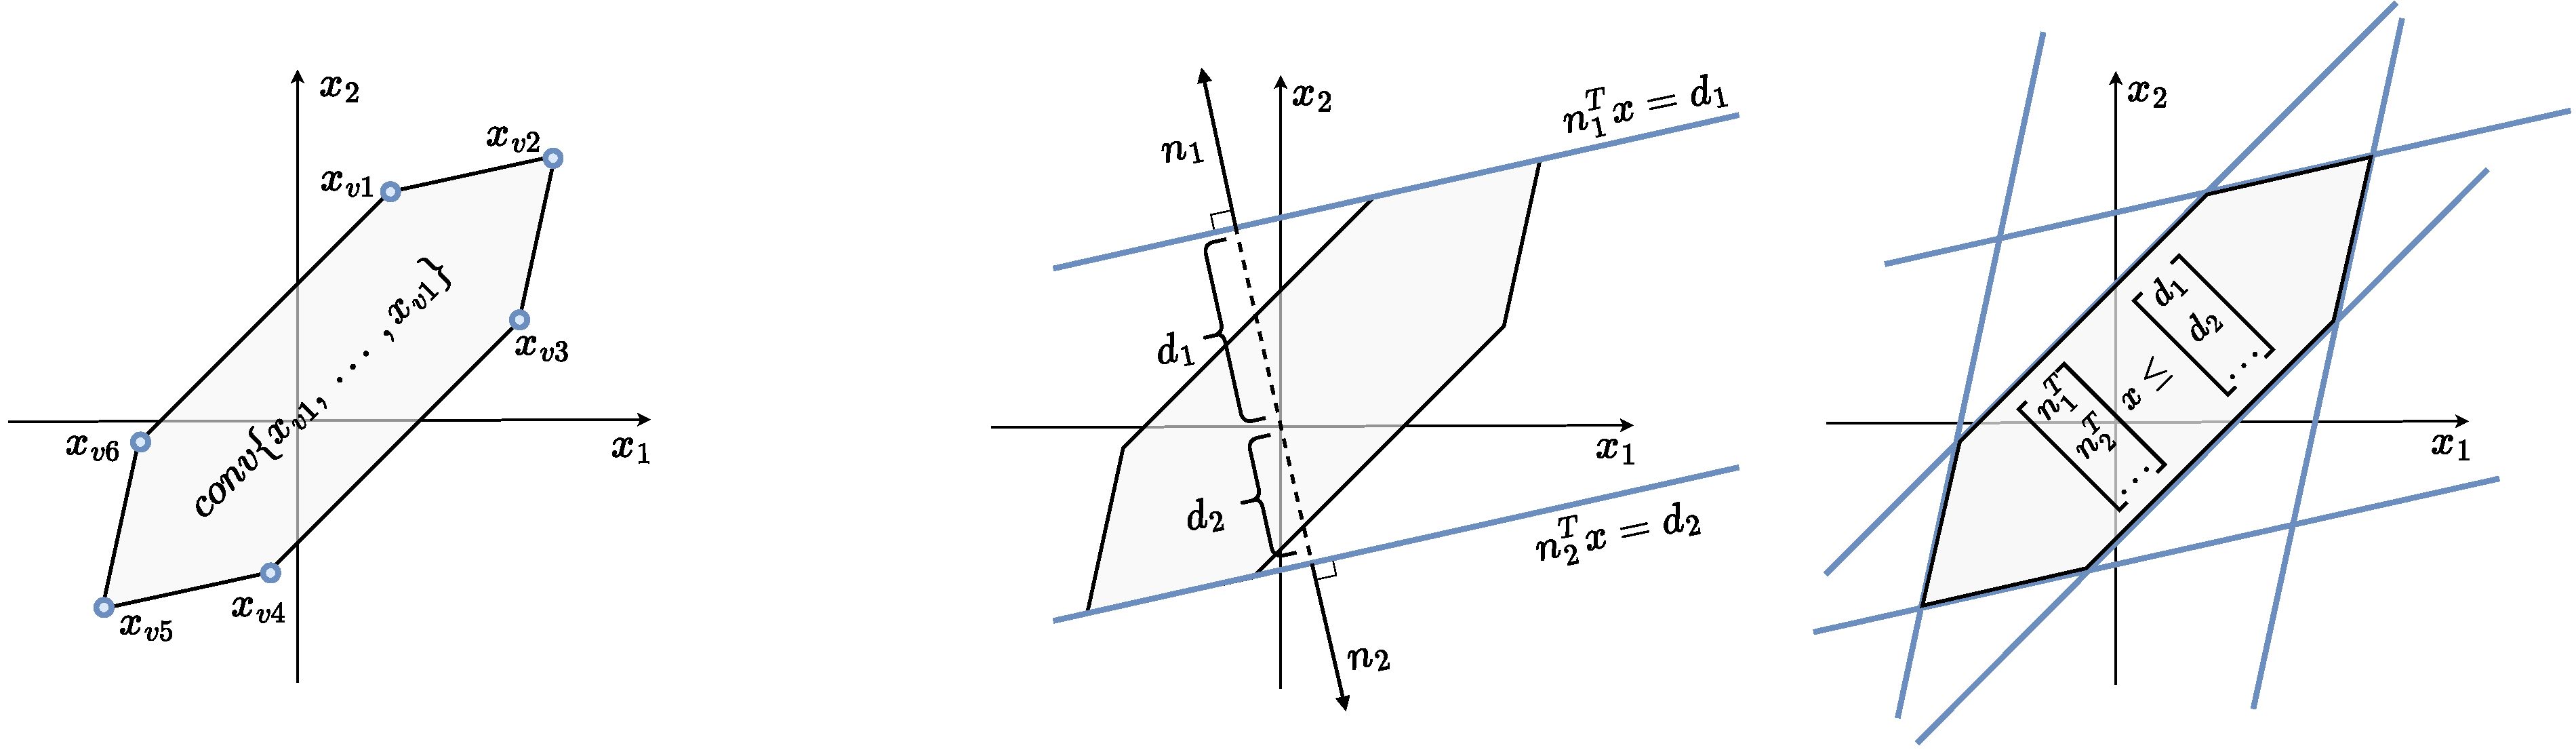
\includegraphics[width=\linewidth]{Chapters/imgs/h_v_rep.pdf}
    \caption{Caption}
    \label{fig:hv_rep}
\end{figure}

Several alternative polytope representations were proposed recently, such as $\repr{Z}$-representation \cite{kochdumper2019representation} where the polytopes are represented as polynomial zonotopes, and $\repr{M}$-representation \cite{sigl2023mrepresentation} which is a more compact special case of $\repr{Z}$-representation. These representations offer an improved efficiency of conducting polytope algebra operations, with respect to the traditional $\repr{H}$ and $\repr{V}$-representations. However, despite these advancements, their practical applications are still quite limited, primarily due to the challenging computational complexity involved in transforming polytopes into these alternative representations. 

Representing polytopes in these standard forms enables using different efficient tools form the computational geometry and polytope algebra to perform operations over polytopes and provides tools for exploiting them in practical applications. However, in many cases polytope formulations do not correspond to neither $\repr{V}$ or $\repr{H}$-representation, as a result, many algorithms are developed in the literature transforming different polytope formulations in one of the two standard forms. The algorithms transforming the polytopes to the $\repr{V}$-representation are often called \textit{vertex enumeration} algorithms and to the $\repr{H}$-representation of are called \textit{facet enumeration} algorithms\cite{bremner_fukuda_marzetta_1998}. The appropriate choice of suitable polytope transformation algorithm, and its complexity, depends on various factors such as the polytope formulation, the desired polytope representation ($\repr{V}$ or $\repr{H}$), and potentially the time constraints for algorithm execution (online or offline). 

Therefore, following section (section \ref{ch:generic_view}) brings a structured overview of different polytopes, especially the ones occurring when characterising different physical abilities of humans and robots, and classifies them with respect to their formulation. Section \ref{ch:polytope_algorithms} then exploits this classification to provide an overview of their applicable polytope transformation strategies and briefly discusses their efficiency.

\section{Generic view of polytope formulations}
\label{ch:generic_view}

To effectively utilise polytopes of physical abilities in practical applications, it is necessary to transform them into standard representations such as $\repr{H}$ or $\repr{V}$-representation. While many algorithms have been proposed in the literature for manipulating polytope representations, they are often created for specific polytope formulations. Hence, this section aims to present a generic perspective on different families of polytope formulations commonly found when characterising the physical abilities of humans and robots. With the goal to categorise these polytopes based on their formulation facilitating the choice of applicable algorithms.

From a generic standpoint, physical abilities represented in a shape of polytopes $\mathcal{P}_x$ can seen as feasible sets of output (task space) variables $\bm{x} \in \mathbb{R}^m$, produced by applying a linear transformation on the input (actuation space) variables $\bm{y} \in \mathbb{R}^n$, bounded within (actuator limits) $\bm{y}\in\mathcal{P}_y$. As described in the previous chapter (section \ref{ch:collab_metrics_overview}), the polytope formulations for characterising physical abilities can be expressed in a unified generic form 
\begin{equation}
    \mathcal{P}_x = \{\bm{x}\in\mathbb{R}^m ~|~ A\bm{x}=B\bm{y} + \bm{b}, ~ \bm{y}\in\mathcal{P}_y\}
    \label{eq:generic_polyt_view_revisit}
\end{equation}
where matrices $B\in\mathbb{R}^{k\times n}$ and $A\in\mathbb{R}^{k\times m}$ present the linear transformation of the $n$ dimensional input to $m$ dimensional output space, through the $k$ dimensional intermediate space, while $\bm{b}\in\mathbb{R}^k$ is a bias vector. Furthermore, the dimensions of output space $m$ is lower than the intermediate space dimension $k\!\geq\! m$ , which is in term lower than the input space dimension $n\!\geq\! k\!\geq\! m$. 

This compact and implicit formulation represents a unified view of different physical ability polytope formulations. However, depending on the structure of the matrices $A$ and $B$, as well as the form of the input set $\mathcal{P}_y$, different algorithms are required to transform this formulation to its standard representations ($\repr{H}$ and $\repr{V}$). 

%Therefore, this section proposes a structured view on different subfamilies of the generic formulation (\ref{eq:generic_polyt_view_revisit}) that can be used with standard polytope transformation (vertex and facet enumeration) algorithms. 

% In order to establish these families two main forms of the input set are considered: interval form $\mathcal{I}_y$ and polytope form $\mathcal{P}_y$. As well as two main structures of the linear transformation equation $A\bm{x}\!=\!B\bm{y}\! +\! \bm{b}$ : \textit{projection} formulation, where matrix $A$ is identity matrix $A=I_{m\times m}$, and \textit{intersection} formulation, where matrix $B$ is identity matrix $B=I_{n\times n}$.

One important factor determining the complexity of the polytope transformation, and the choice of the suitable algorithm, is the shape of the input set, corresponding to the limits of the input variable $\bm{y}\in\mathbb{R}^n$ limits. There are two most common forms that can be considered: interval form $\mathcal{I}_y$ and polytope form $\mathcal{P}_y$. 

The interval shaped $\mathcal{I}_y$ input set is specified in a form of min-max intervals
\begin{equation}
    \mathcal{I}_y = \{\bm{y}\in \mathbb{R}^n |~~ \bm{y}_{min} \leq \bm{y}\leq \bm{y}_{max} \}
    \label{eq:hypercube_lim}
\end{equation}
In a geometric sense, these individual intervals of the input variable $\bm{y}$ can be visualised as an $n$-dimensional hyperrectangle, also known as a hyperbox or an orthotope. Each axis $i$ of the hyperrectangle corresponds to an interval $y_i\in[y_{i,\text{min}},y_{i,\text{max}}]$.

In general case, rather than interval $\mathcal{I}_y$, the input set can be defined as any convex polytope (ex. set of linear constraints in its $\repr{H}$-representation).
\begin{equation}
    \mathcal{P}_y = \{\bm{y}\in \mathbb{R}^n|~~ H_y\bm{y}\leq \bm{d}_y \}
\end{equation}

As polytopes $\mathcal{P}_x$ are then defined as linear transformations $A\bm{x}\!=\!B\bm{y}\! +\! \bm{b}$ of the input set (intervals $\mathcal{I}_y$ or polytope $\mathcal{P}_y$ shaped) from the input space to the output space, the structure of the linear transformation (matrices $A$ and $B$) has a direct impact on the complexity of the formulation, as well as on the choice of the algorithm.
Therefore, in this work, the distinction between two generic families of polytope formulations is proposed, derived from the unified formulation (\ref{eq:generic_polyt_view_revisit}): \textit{projection} formulation, where matrix $A$ is identity matrix $A=I_{m\times m}$, and \textit{intersection} formulation, where matrix $B$ is identity matrix $B=I_{n\times n}$.

\subsection{Projection formulation}
\label{ch:proj_formulaiton}

\begin{figure}[!h]
    \centering
    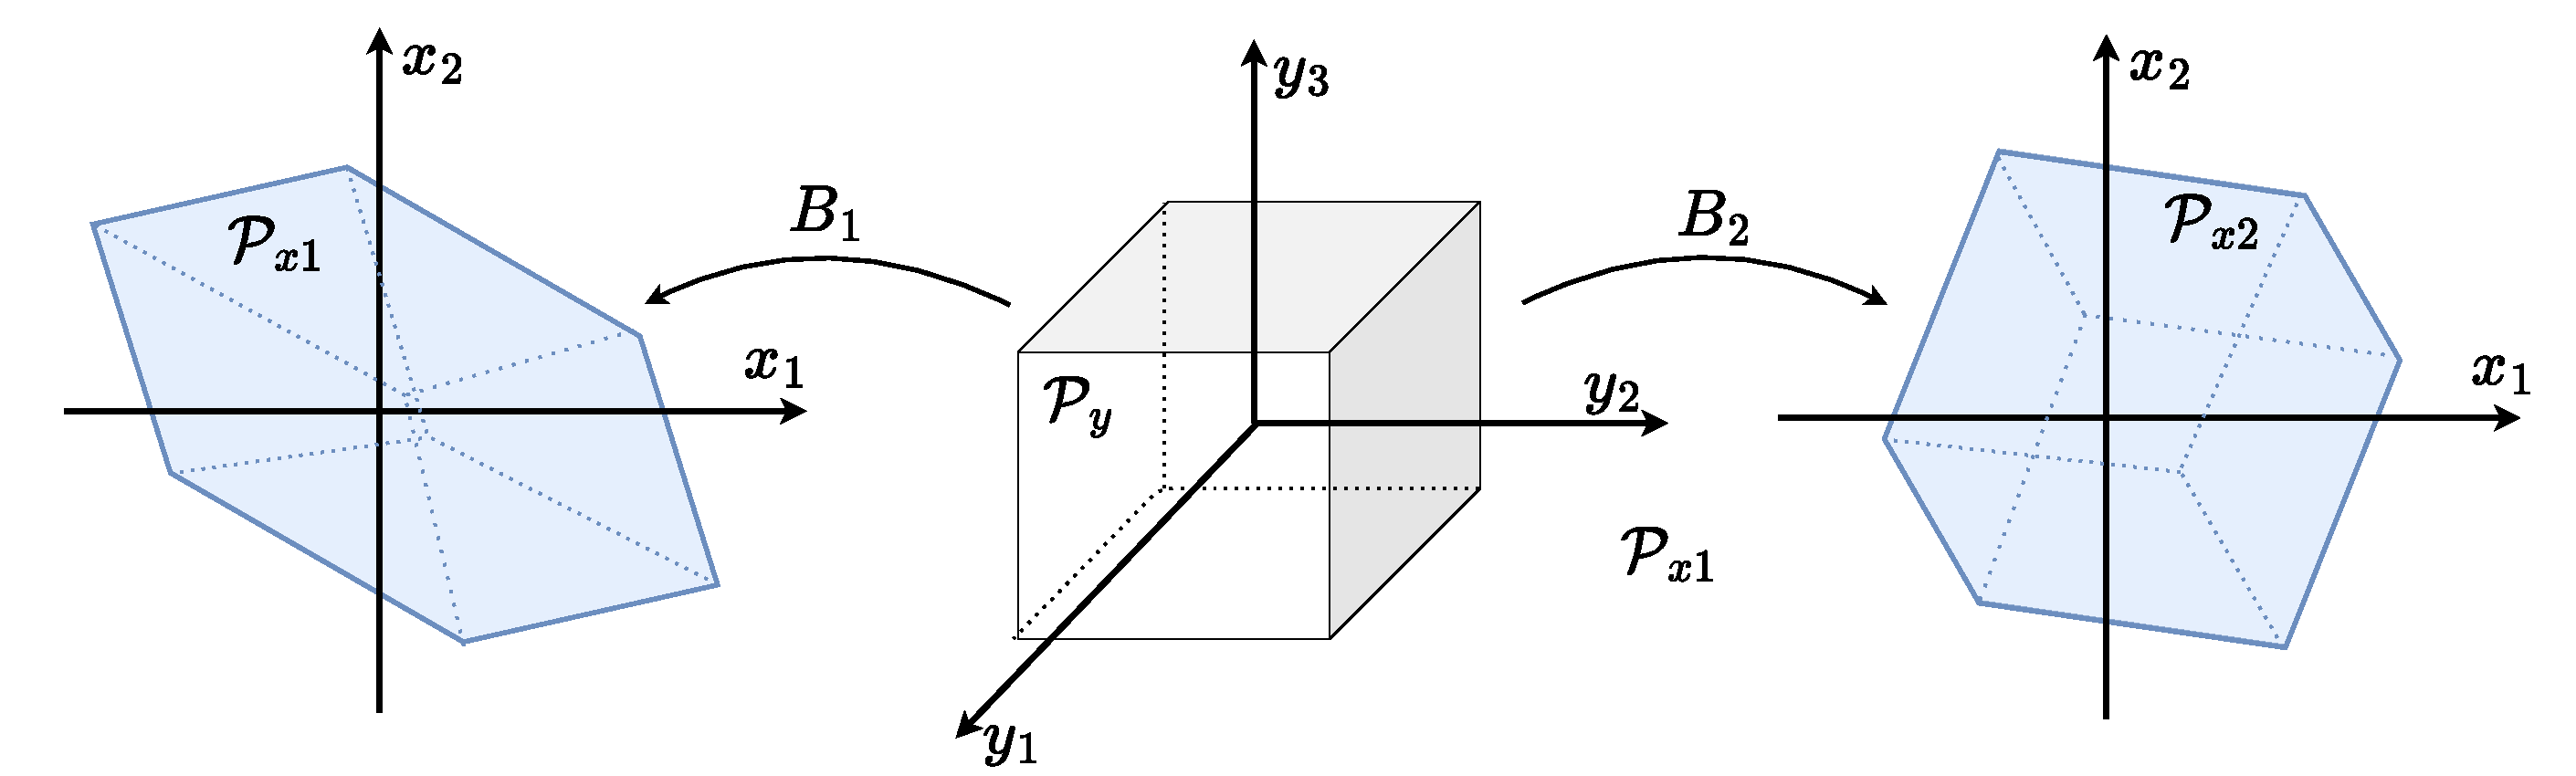
\includegraphics[width=0.8\linewidth]{Chapters/imgs/projection_double.pdf}
    \caption{An example ($m=2$, $n=3$) of constructing two different projection formulation polytopes, from the same input set $\mathcal{P}_y$. Polytopes $\mathcal{P}_{x1}$ and $\mathcal{P}_{x2}$ represent linear affine transformations of the input set $\mathcal{P}_y$ using two different transformation matrices $B_1$ and $B_2$.}
    \label{fig:proj_zono}
\end{figure}

Projection formulation is defined through a linear affine transformation of the $n$ dimensional input space $\bm{y}\in\mathbb{R}^n$ to the $m$ dimensional output space $\bm{x}\in\mathbb{R}^m$ using the projection matrix $B\in \mathbb{R}^{m\times n}$
\begin{equation}
    \mathcal{P}_x=\{\bm{x}\in \mathbb{R}^m ~|~ \bm{x} = B\bm{y} + \bm{b}_x,~\bm{y} \in\mathcal{P}_y \}
    \label{eq:proj_poly}
\end{equation}
where $\bm{b}_x\in\mathbb{R}^m$ is a constant bias vector, defined in the output space. The name \textit{projection} formulation comes from the fact that the polytope $\mathcal{P}_x$ in this formulation is a projection of the $n$ dimensional input set $\mathcal{P}_y$ to the (usually lower) $m$ dimensional output space $\mathbb{R}^m$ \cite{Burger1996projection}.

A graphical representation of the projection formulation (\ref{eq:proj_poly}) is shown on Figure \ref{fig:image_projection_two}, where two different output polytopes $\mathcal{P}_x$ are constructed applying different affine transformation matrices $B$ on the same input set $\mathcal{P}_x$.


\paragraph*{Zonotope formulation} If the input space has the interval shape $\mathcal{I}_y$, the final polytope $\mathcal{P}_x$, defined by the equation (\ref{eq:proj_poly}), has a Zonotope form. In that case the polytope $\mathcal{P}_x$ can be represented as a Minkowski sum of $n$ line segments $\mathcal{L}_i$, each one corresponding to one axis range $[y_{i,min}, y_{i,max}]$ of the input set $\mathcal{I}_y$ projected to the output space using the matrix $B$.  \cite{McMullen1971onzonotopes}

\begin{equation}
    \mathcal{P}_x = \mathcal{L}_1 \oplus~ \cdots ~\oplus \mathcal{L}_n
\end{equation}
where the $i$-th line segment $\mathcal{L}_i$ can be expressed through $i$-th line vector $\bm{b}_i$ of the matrix $B$
\begin{equation}
    \mathcal{L}_i = \{\bm{x}\in\mathbb{R}^m ~|~ \bm{x} = \bm{b}_iy_i + \bm{b}_x,~~ y_i\in [y_{i,min}, y_{i,max}] \}
\end{equation}
\begin{wrapfigure}{r}{0.5\linewidth}
    \centering
    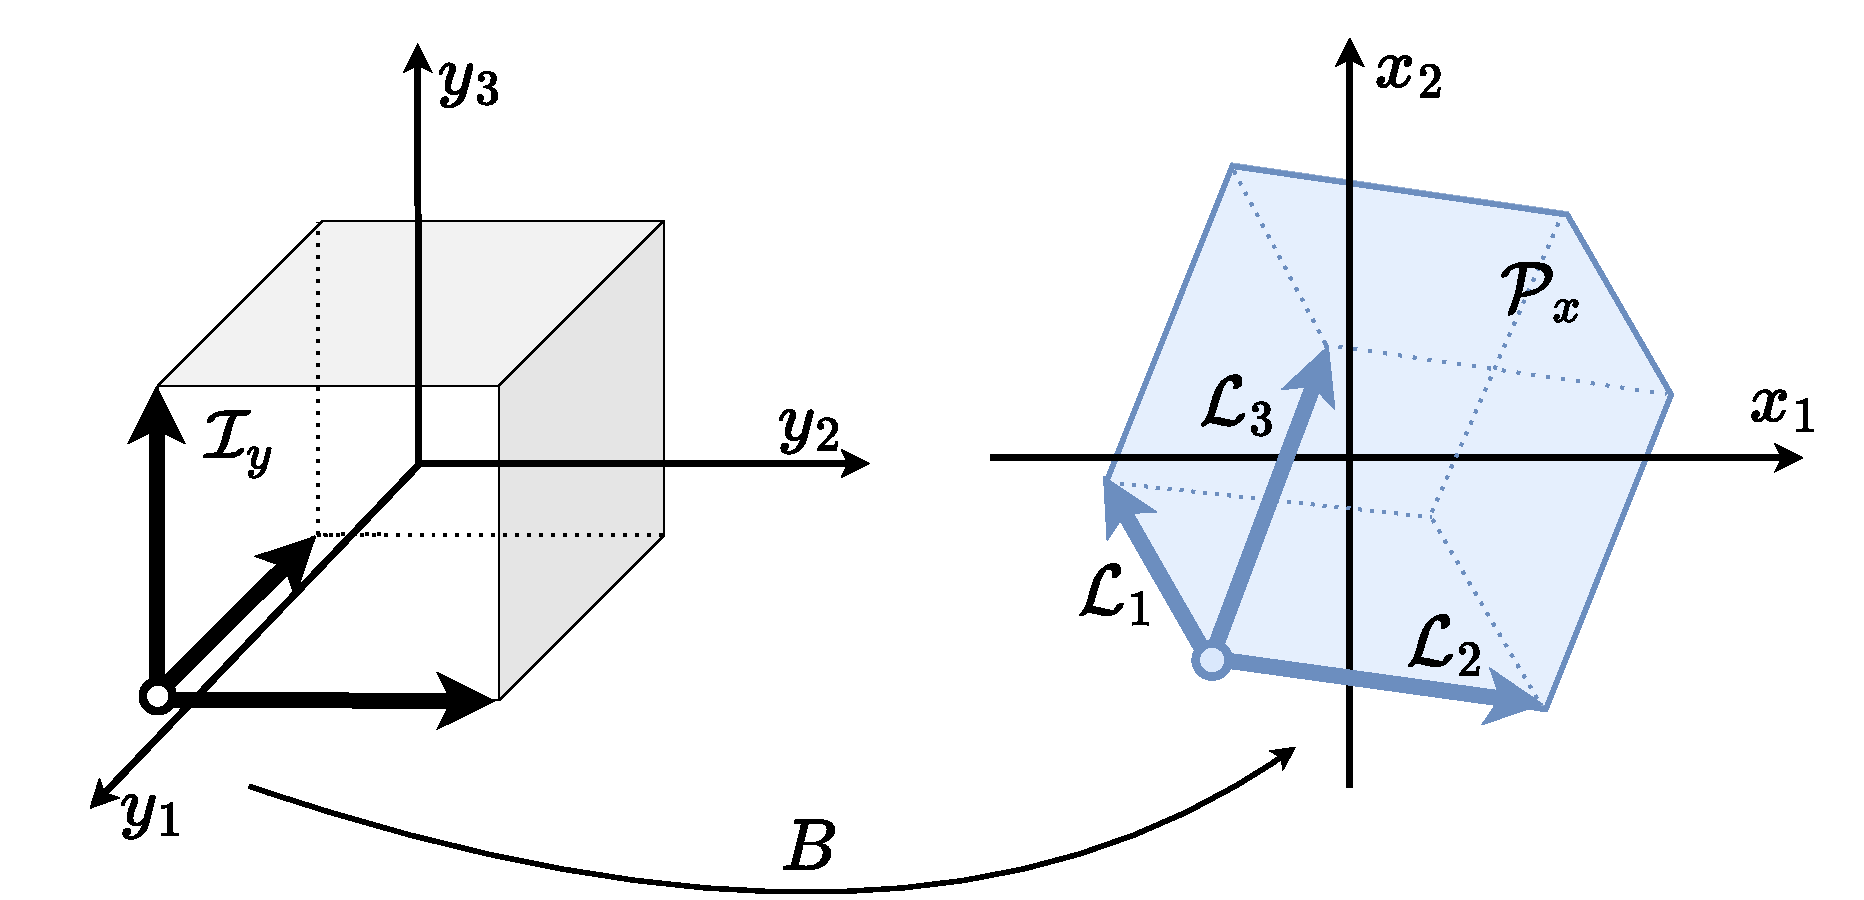
\includegraphics[width=\linewidth]{Chapters/imgs/zonotope_only.pdf}
    \caption{A graphical example ($m=2$, $n=3$) of constructing the Zonotope shaped polytope $\mathcal{P}_x$ from the interval input set $\mathcal{I}_y$.}
    \label{fig:image_projection_two}
\end{wrapfigure}
These line segments are often called \textit{components} or \textit{generators} of the Zonotope $\mathcal{P}_x$. \cite{shephard1974zonotopes}.

Furthermore, for any Zonotope shaped input set $\mathcal{P}_y$, polytope $\mathcal{P}_x$ is a Zonotope as well. And it can be expressed as a Minkowski sum of the generators $\mathcal{L}_{yi}$ of the input set $\mathcal{P}_y$
\begin{equation}
    \mathcal{P}_y = \mathcal{L}_{y1}  ~\oplus \mathcal{L}_{y2}~\oplus~ \cdots
\end{equation}
, projected to the output space using the equation (\ref{eq:proj_poly}). The polytope $\mathcal{P}_x$ will has the same number of generators as the Zonotope $\mathcal{P}_y$, and they can be expressed as
\begin{equation}
    \mathcal{L}_i = \{\bm{x}\in\mathbb{R}^m ~|~ \bm{x} = B\bm{y} + \bm{b}_x,~~ \bm{y}\in  \mathcal{L}_{yi}\}
\end{equation}

Zonotopes are highly structured and central symmetric shapes, hence transforming them to appropriate representations ($\repr{H}$ and $\repr{V}$) is in many cases more efficient than for generic polytopes.


\subsection{Intersection formulation}
\label{ch:inter_formulaiton}

\begin{figure}[!h]
    \centering
    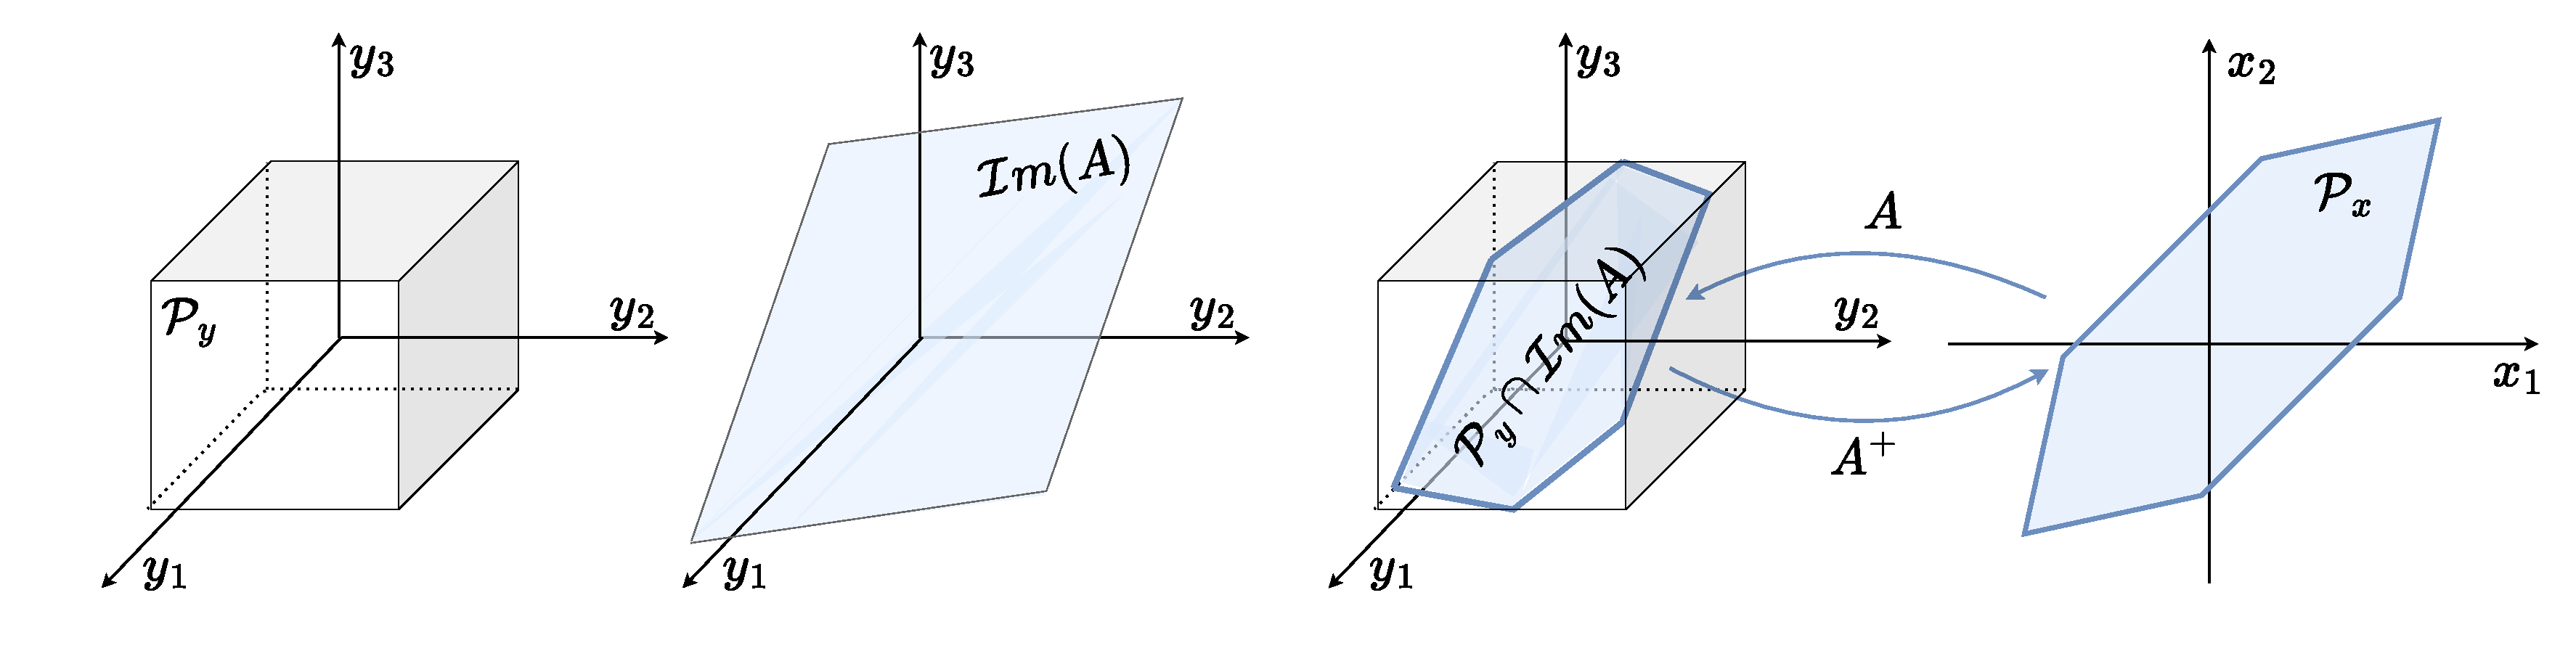
\includegraphics[width=\linewidth]{Chapters/imgs/image_intersection_poly_all.pdf}
    \caption{An example ($m=2$, $n=3$) of constructing a intersection formulation polytope $\mathcal{P}_x$ from the input set $\mathcal{P}_y$. First the image $\img{A}$ of the matrix $A$ is intersected with the input set $\mathcal{P}_y$, then this intersection is projected to the output space using the pseudo-inverse $A^+$. }
    \label{fig:inter_image_poly}
\end{figure}
Intersection formulation, on the other hand, is expressed by a matrix equation $A\bm{x}=\bm{y}$, which can be interpreted as a linear transformation in the opposite direction\cite{LARSON2013}, from the $m$ dimensional input space $\bm{x}\in\mathbb{R}^m$ to the $n$ dimensional output space $\bm{y}\in\mathbb{R}^n$, using the projection matrix $A\in \mathbb{R}^{n\times m }$
\begin{equation}
    \mathcal{P}_x=\{\bm{x} \in \mathbb{R}^m|~ A\bm{x} = \bm{y}+ \bm{b}_y,~ \bm{y} \in \mathcal{P}_y\}
    \label{eq:inter_poly}
\end{equation}
where $\bm{b}_y \in \mathbb{R}^n$ is a constant bias vector, defined in the input space. The name \textit{intersection} formulation comes from the fact that the polytope $\mathcal{P}_x$ is no longer just a projection of the input set $\mathcal{P}_y$ to the $m$ dimensional output space, but rather a projection of its intersection with the image $\img{A}$ of the matrix $A$. 
A graphical representation of the intersection formulation (\ref{eq:inter_poly}) is shown on Figure \ref{fig:inter_image_poly}, where the intersection $\mathcal{P}_y\cap \img{A}$ and the final polytope $\mathcal{P}_x$ are denoted in blue.

The main difficulty of the intersection formulation (\ref{eq:inter_poly}) is that it is defined as an inverse projection, from the $m$ dimensional output space to the $n$ dimensional input space\cite{LARSON2013}. In order to inverse this relationship, an equivalent projection formulation polytope can be constructed by characterising the intersection $\mathcal{P}_y\cap \img{A}$. 

\paragraph*{Equivalent projection formulation}\label{par:equivalent_proj} In order to express the intersection formulation in the projection form, it is necessary to inverse the relationship $\bm{y}=A\bm{x}$, considering $\bm{b}_y=\bm{0}$. If the input and output space have the same dimension $n=m$, matrix $A$ is invertible and the inverse relationship can be easily obtained as $\bm{x} = A^{-1}\bm{y}$. 


However, in more general case, the input space is higher dimensional $n>m$, making the matrix $A$ not invertible. In such cases the inverse relationship can be obtained using the left pseudo-inverse of the matrix $A$
\begin{equation}
    \bm{x} = (A^TA)^{-1}A^T\bm{y} = A^+\bm{y}
    \label{eq:pseudoinverse_equation}
\end{equation}

\begin{wrapfigure}{r}{0.45\linewidth}
    \centering
    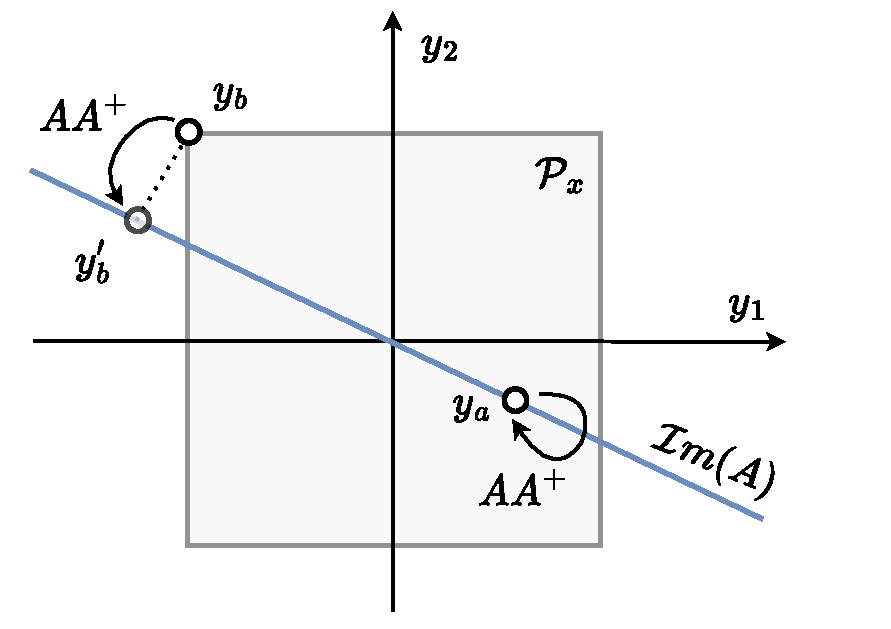
\includegraphics[width=\linewidth]{Chapters/imgs/img_pseudo_prob.pdf}
    \caption{An example ($n=2$,$m=1$) of applying the image projector $AA^+$ in the input space, the input set $\mathcal{P}_y$ is shown in grey and the image $\img{A}$ in blue. As the input vector $\bm{y}_a$ belongs to the image $\img{A}$ its multiplication with $AA^+$ results in the same vector. $\bm{y}_b$  does not belong to the image and $AA^+$ results in $\bm{y}_b'$, its orthogonal projection onto the image $\img{A}$, however outside the input set $\mathcal{P}_y$.}
    \label{fig:image_psueodinverse_ilustration}
\end{wrapfigure}
Due to the fact that in general case the operation $\bm{x}=A^+\bm{y}$ is not bijective, the input vector $\bm{y}'=A\bm{x}$ corresponding to the output vector $\bm{x}=A^+\bm{y}$, in general case, does not correspond to the original input vector $\bm{y}$ 
\begin{equation}
\bm{y}' = A\bm{x} = A(A^+\bm{y})\neq\bm{y}
\end{equation}
making it possible that the input vector $\bm{y}'=AA^+\bm{y}$ no longer respects the input set $\mathcal{P}_y$
\begin{equation}
    \bm{y}'=AA^+\bm{y}\notin\mathcal{P}_y
\end{equation}

The matrix $AA^+$ represents an orthogonal projector matrix to the \textit{image space} $\img{A}$ of the matrix $A$ \cite[Chapter 5.5.4]{golub1996matrix}. Thererfore, for any input vector $\bm{y}$ belonging to the image $\img{A}$, the multiplication by $AA^+$ results in itself \cite[Chapeter 1.3.1]{wang2018generalized}
\begin{equation}
    \bm{y} = AA^+\bm{y}, \qquad \forall \bm{y}\in\img{A}
\end{equation}
However, for any input vector $\bm{y}$ not belonging to the image $\img{A}$, multiplying it with the matrix $AA^+$ will result in its orthogonal projection to the image $\img{A}$. As shown in the graphical example on Figure \ref{fig:image_psueodinverse_ilustration}, even though the original $\bm{y}$ respects the input set $\mathcal{P}_y$, its orthogonal projection onto the image $AA^+\bm{y}$ is some cases does not.

Therefore, by ensuring that all the inputs $\bm{y}$ belong to the image $\img{A}$, the pseudo-inverse $A^+$ provides a unique inverse solution to the equation $\bm{y} = A\bm{x}$. Then, the new input set, respecting the limitations $\bm{y}\in\mathcal{P}_y$ and ensuring the unique inverse solution, can be can be found as the intersection
\begin{equation}
   \bm{y} \in \img{A} \cap \mathcal{P}_y
    \label{eq:intersection_ai}
\end{equation}
By exploiting the new input set and using the pseudo-inverse $A^+$, the equivalent formulation of the the initial intersection polytope $\mathcal{P}_x$ can be expressed as
\begin{equation}
\mathcal{P}_x=\{\bm{x}\in\mathbb{R}^m~|~ \bm{x} = A^+\bm{y} + A^+\bm{b}_y,~ \bm{y} \in \img{A}\cap\mathcal{P}_y\} \label{eq:proj_inter}
\end{equation}

The relationship between the pseudo-inverse and the image $\img{A}$ is discussed more in detail in appendix \ref{ch:pseudoinverse_unique}, while appendix \ref{ch:image_char} demonstrates the characterisation of the image space , $\bm{y}\in\img{A}$, in a set form. 


Figure \ref{fig:inter_image_poly} shows a graphical representation of this mapping where the intersection $ \img{A}\cap\mathcal{P}_y$ is shown in blue, as well as the final polytope $\mathcal{P}_x$ being its projection to the output space $\bm{x}\in \mathbb{R}^m$. 

Therefore, the intersection formulation is generally more computationally complex to work with, than the projection formulation, as it often requires characterising the intersection $\img{A}\cap\mathcal{P}_y$.  The graphical comparison of the construction of both intersection and projection polytopes from the same input set is shown on Figure \ref{fig:inter_proj}.


\begin{figure}
    \centering
    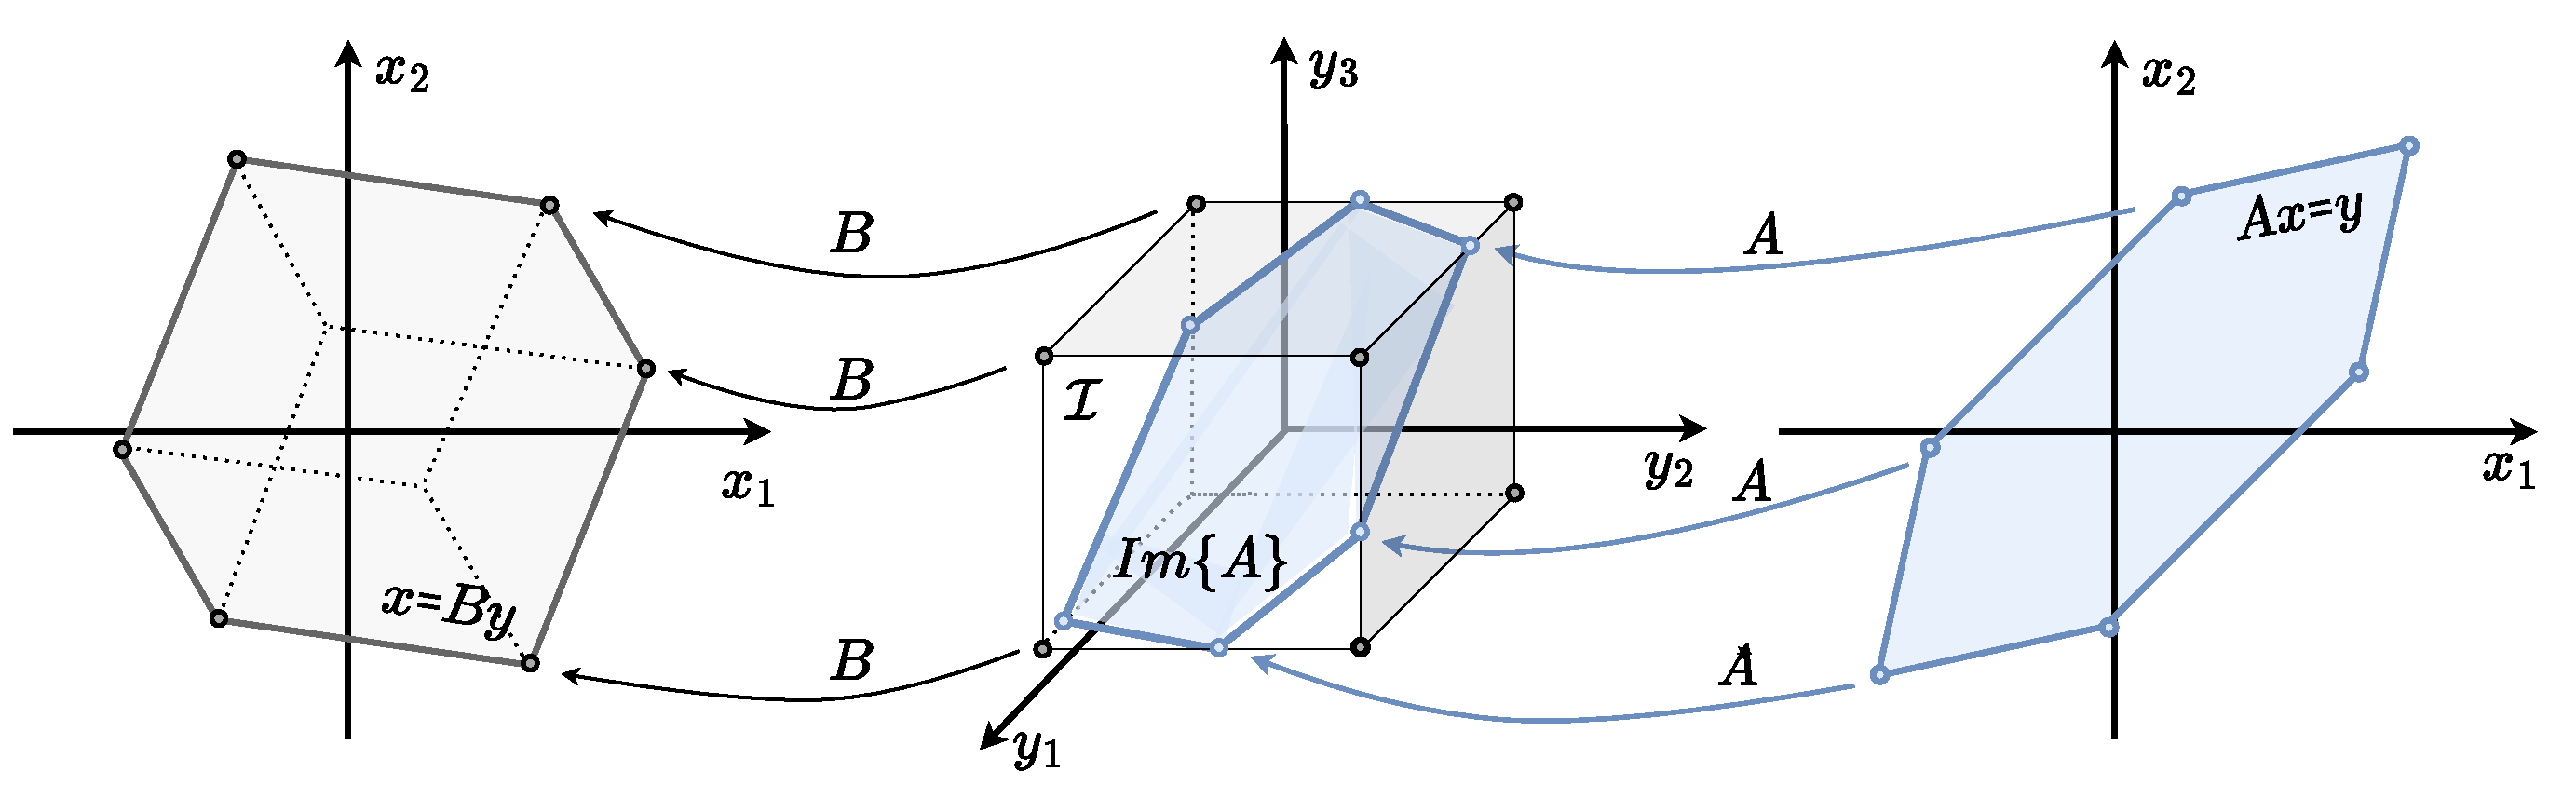
\includegraphics[width=\linewidth]{Chapters/imgs/intersection_projection.pdf}
    \caption{A comparative view of the projection (left) and intersection (right) polytope formulation using the same input space (middle). In the projection formulation, the whole input space $\mathcal{P}_y$ is projected using the matrix $B$ to the output space to obtain the polytope $\mathcal{P}_x$ (gray left). In the intersection formulation, first the intersection of the input space $\mathcal{P}_y$ with the image of the matrix $A$ has to be found (blue middle) $\img{A} \cap \mathcal{P}_y$ , then this intersection can be projected to the output space using the pseudo-inverse $A^+$ of the matrix $A$ to obtain the polytope $\mathcal{P}_x$ (blue right).}
    \label{fig:inter_proj}
\end{figure}

\subsection{Special cases}
\label{ch:combined_forms}
Physical ability metrics described in chapter \ref{ch:poly_metrics} contain two special cases of polytope formulations that combine both intersection and projection formulations: \textit{intersection-projection} and \textit{projection-intersection} formulation.

\subsubsection{Intersection-projection formulation}
\label{ch:inter_proj_form}

This special case of the polytope formulation contains both intersection and projection formulation
\begin{equation}
    \mathcal{P}_x \in \{\bm{x}\in \mathbb{R}^m~|~\underbrace{A \bm{x}= \bm{z}+ \bm{b}_z}_{\text{intersection}},~ \underbrace{ \bm{z}=B \bm{y}}_{\text{projection}} ,~ \bm{y} \in \mathcal{P}_y\} 
    \label{eq:inter_proj_poly}
\end{equation}
where $\bm{x}\in\mathbb{R}^m$ is the output vector, $\bm{y} \in \mathbb{R}^n$ is an input vector and $\bm{z}\in\mathbb{R}^k$ is an intermediate space vector, where $n\!\geq\!k\!\geq\!m$. Matrix $B\in \mathbb{R}^{k \times n}$ is a projector matrix from $n$ dimensional input space to the $k$ dimensional intermediate space, matrix $A\in \mathbb{R}^{k\times m}$ is a projector matrix from $m$ dimensional output space to the $k$ dimensional intermediate space and $\bm{b}_z\in\mathbb{R}^k$ is the bias vector, defined in the intermediate space.

In this work, this polytope formulation is named \textit{intersection-projection} as it is a special case of a intersection formulation (\ref{eq:inter_poly}) with polytope shaped input set which has the projection formulation. The final polytope $\mathcal{P}8x$ can be expressed as
\begin{equation}
    \mathcal{P}_x \in \{\bm{x}\in \mathbb{R}^m~|~A \bm{x} = \bm{z} + \bm{b}_z,~ \bm{z} \in \mathcal{P}_z\} 
\end{equation}
where its input set polytope $\mathcal{P}_z$ is defined using the projection formulation
\begin{equation}
    \mathcal{P}_z \in \{\bm{z}\in \mathbb{R}^k~|~z = B\bm{y},~ \bm{y} \in \mathcal{P}_y\} 
\end{equation}

\begin{figure}[!t]
    \centering
    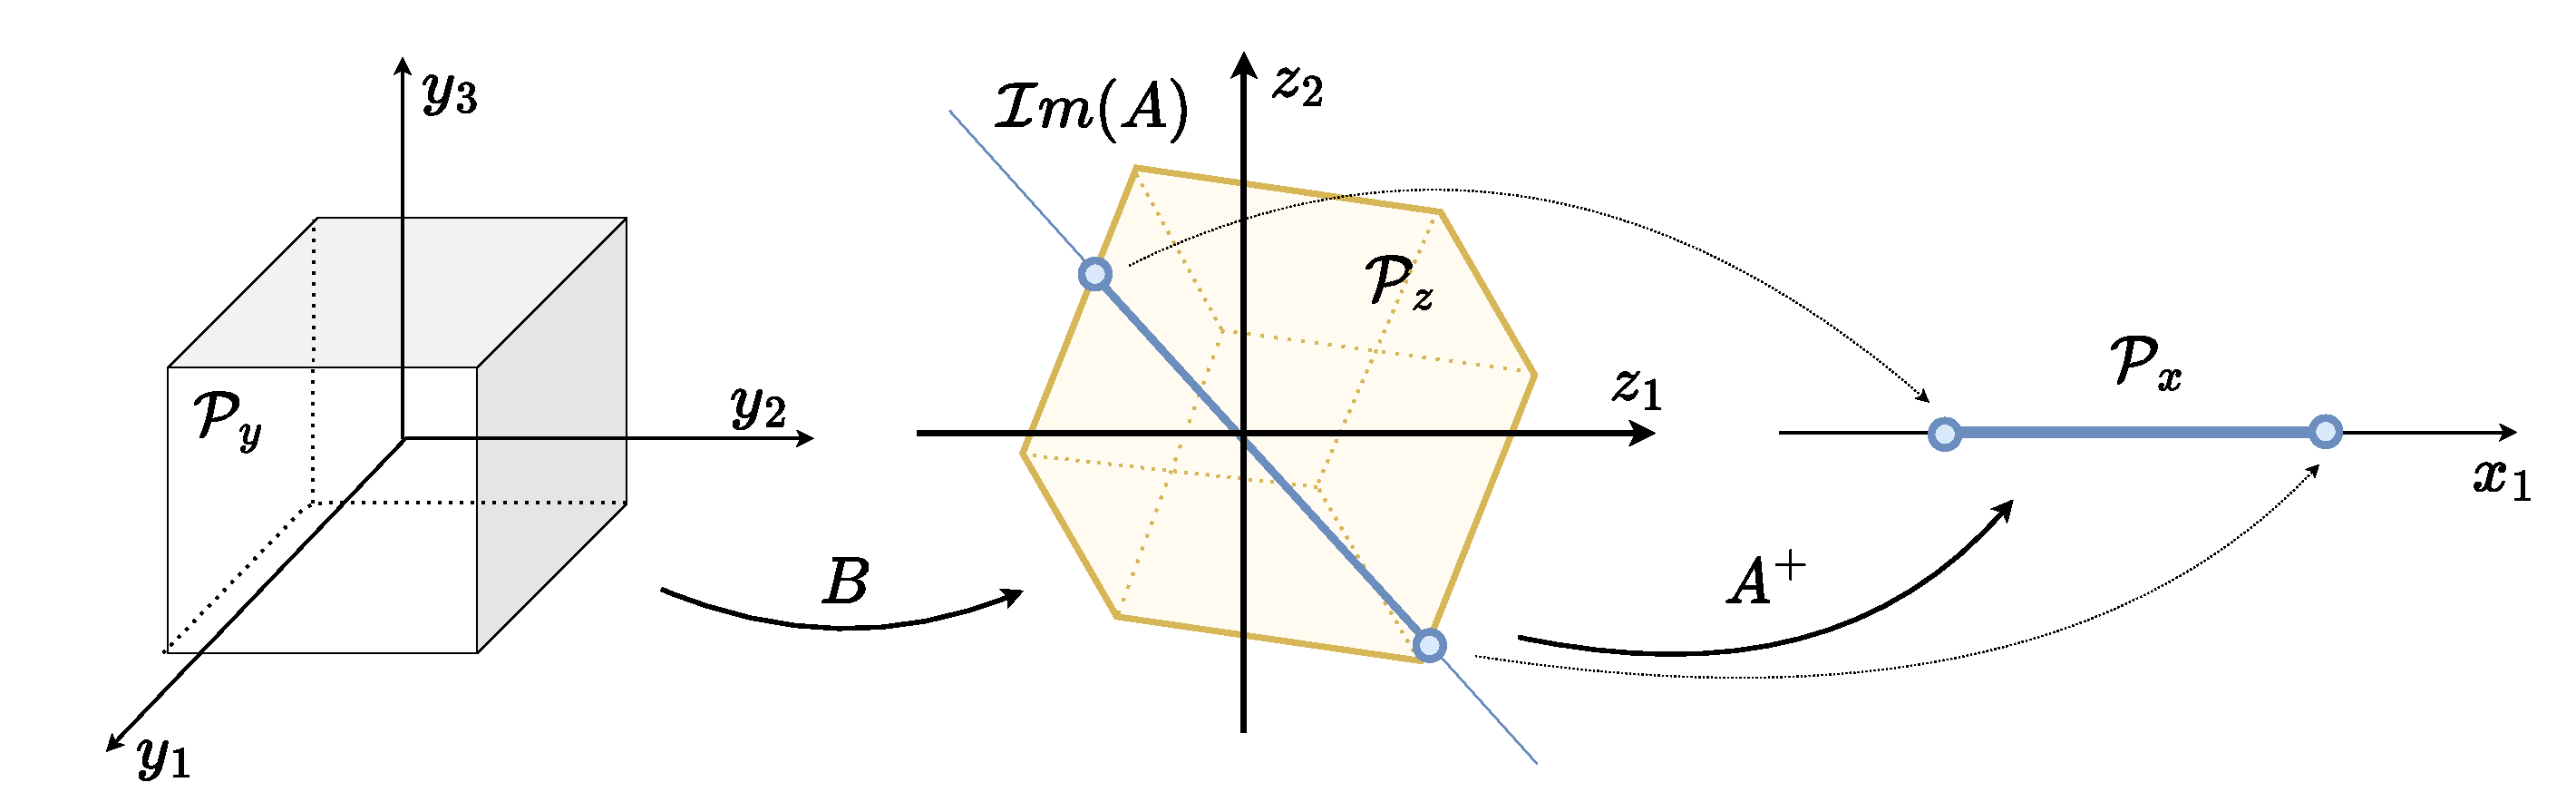
\includegraphics[width=\linewidth]{Chapters/imgs/spec_int_proj.pdf}
    \caption{An example ($n=3$, $k=2$, $m=1$) of a construction of the intersection-projection polytope $\mathcal{P}_x$ from the input set $\mathcal{P}_y$. Geometrically, first the input set $\mathcal{P}_y$ is projected to the intermediate space $\mathbb{R}^k$ to obtain the projection polytope $\mathcal{P}_z$ (yellow). Then this polytope is intersected with the image $\img{A}$ of matrix $A$ (blue middle). Finally the intersection $\mathcal{P}_z\cap\img{A}$ is projected to the output space with the pseudo-inverse $A^+$ to obtain the final 1D polytope $\mathcal{P}_x$ (blue right).}
    \label{fig:inter_proj_spec}
\end{figure}
This formulation can also be transformed to an equivalent projection formulation, as described for intersection formulation is section \ref{par:equivalent_proj}, resulting in a polytope 
\begin{equation}
\mathcal{P}_x=\{\bm{x} \in \mathbb{R}^m |~ \bm{x} = A^+\bm{z} - A^+\bm{b}_z,~ \bm{z}+\bm{b}_z \in \img{A}\cap\mathcal{P}_z\} 
\end{equation}

However, this polytope formulation is much more computationally complex than both intersection and projection formulation, as it requires first computing the projection polytope $\mathcal{P}_z$ and then finding the intersection $\img{A}\cap\mathcal{P}_z$ in order to find the polytope $\mathcal{P}_x$. A graphical example of constructing the intersection-projection formulation polytope is shown on Figure \ref{fig:inter_proj_spec}.


\begin{remark}
    This generic formulation corresponds to the formulations of the wrench and stiffness capacity polytopes for human musculoskeletal models, described in the sections \ref{ch:force_poly_human} and \ref{ch:human_stiffness_poly}.
\end{remark}


\subsubsection{Projection-intersection formulation}

A different special case of polytope formulation combining both projection and intersection formulation can be expressed as 
\begin{equation}
    \mathcal{P}_x \in \{\bm{x}\in \mathbb{R}^m~|~ \underbrace{\bm{x} = B \bm{z} + \bm{b}_x}_{\text{projection}},~ \underbrace{A\bm{z}=\bm{y}}_{\text{intersection}},~ \bm{y} \in \mathcal{P}_y\} 
    \label{eq:proj_inter_poly}
\end{equation}
where $\bm{x}\in\mathbb{R}^m$ is the output vector, $\bm{y} \in \mathbb{R}^b$ is an input vector and $\bm{z}\in\mathbb{R}^k$ is an intermediate space vector, where $n\!\geq\!k\!\geq\!m$. Matrix $A\in \mathbb{R}^{k \times n}$ is a projector matrix from $n$ dimensional input space to the $k$ dimensional intermediate space, matrix $B\in \mathbb{R}^{m\times k}$ is a projector matrix from $k$ dimensional intermediate space to the $m$ dimensional output space and $\bm{b}_x\in\mathbb{R}^m$ is the bias vector, defined in the output space.

In this work, this polytope formulation is named \textit{projection-intersection} as it is a special case of a projection formulation (\ref{eq:proj_poly}) with polytope shaped input set which has the intersection formulation. The final polytope $\mathcal{P}8x$ can be expressed as
\begin{equation}
    \mathcal{P}_x \in \{\bm{x}\in \mathbb{R}^m~|~ \bm{x} = B\bm{z} + \bm{b}_x,~ \bm{z} \in \mathcal{P}_z\} 
\end{equation}
where its input set polytope $\mathcal{P}_z$ is defined using the intersection formulation
\begin{equation}
    \mathcal{P}_z \in \{\bm{z}\in \mathbb{R}^n~|~Az = \bm{y},~ \bm{y} \in \mathcal{P}_y\} 
\end{equation}

This formulation can also be transformed to an equivalent projection formulation, using the same procedure described in section \ref{par:equivalent_proj}, resulting in a polytope 
\begin{equation}
\mathcal{P}_x=\{\bm{x} \in \mathbb{R}^m |~ \bm{x} = BA^+\bm{y} + \bm{b}_x,~ \bm{y}\in \img{A}\cap\mathcal{P}_y\} 
\end{equation}

\begin{figure}
    \centering
    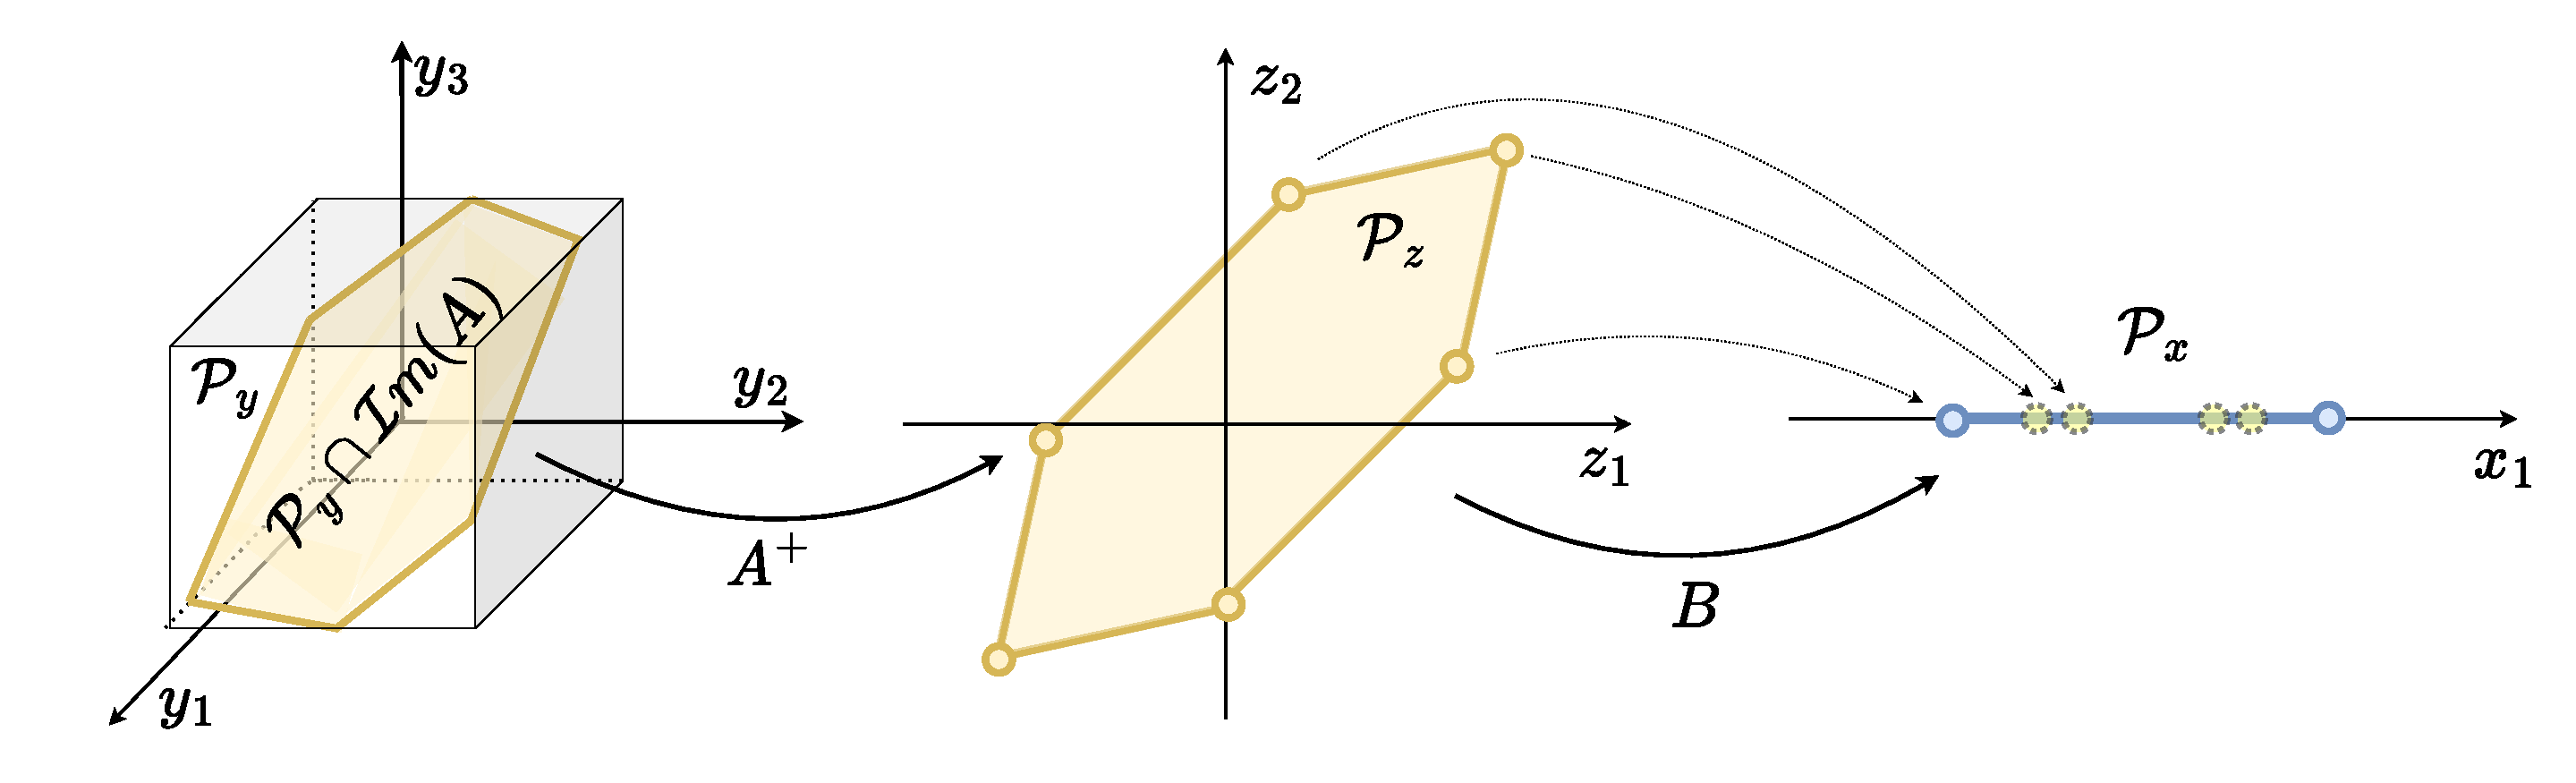
\includegraphics[width=\linewidth]{Chapters/imgs/spec_proj_int.pdf}
    \caption{An example ($n=3$, $k=2$, $m=1$) of a construction of the projection-intersection polytope $\mathcal{P}_x$ from the input set $\mathcal{P}_y$. 
    Geometrically, first the input set $\mathcal{P}_y$ is intersected with the image $\img{A}$ of the matrix $A$ (yellow left). The intersection $\mathcal{P}_y\cap\img{A}$ is then projected to the intermediate space using the pseudo-inverse $A^+$ to obtain the polytope $\mathcal{P}_z$ (yellow middle). Finally, an affine transformation $B$ is applied to the polytope $\mathcal{P}_z$ to transforming it to the final polytope 1D ($m=1$) $\mathcal{P}_x$ (blue right).}
    \label{fig:proj_inter_spec}
\end{figure}
This polytope formulation is again much more computationally complex than both intersection and projection formulation, as it requires first computing the intersection $\bm{y} \in \img{A}\cap\mathcal{P}_y$, followed by the projection $BA^{+}\bm{y}$. A graphical example of constructing the projection-intersection formulation polytope is shown on Figure \ref{fig:proj_inter_spec}.

\begin{remark}
    This generic formulation corresponds to the formulation of the velocity capacity polytope for human musculoskeletal models, described in the section \ref{ch:human_vel_poly}.
\end{remark}


\subsection{Synthesis of polytope formulations}
\label{ch:which_metric_which_formulation}

Section \ref{ch:generic_view} proposes a structured view on different families of polytope formulations, with the aim to group the polytope formulations that can be used with the same polytope transformation algorithms. The discussed families are based on the generic polytope formulation (\ref{eq:generic_polyt_view_revisit}), 
\begin{equation}
    \mathcal{P}_x = \{\bm{x}\in\mathbb{R}^m ~|~ A\bm{x}=B\bm{y} + \bm{b}, ~ \bm{y}\in\mathcal{P}_y\}
    \label{eq:generic_polyt_view_revisit2}
\end{equation}
which, as described in the previous Chapter \ref{ch:phisical_ability_metrics} (synthesis section \ref{ch:collab_metrics_overview}), unifies all the common polytope representations for characterising physical abilities of robots and humans. 

There are two main families of polytope formulations discusses in this section: projection and intersection polytope formulation. 

The projection formulation (\ref{eq:proj_hyp}) corresponds to the specific case of the formulation \ref{eq:generic_polyt_view_revisit2} where the matrix $A$ is an identity matrix $I_{m\times m}$.
The projection formulation is defined as the linear affine transformation of the input set $\mathcal{P}_y$ into the output space through the matrix $B$, forming the polytope $\mathcal{P}_x$. 

The intersection formulation (\ref{eq:inter_poly}) corresponds to the specific case of the formulation 
\ref{eq:generic_polyt_view_revisit2} where the matrix $B$ is an identity matrix $I_{n\times n}$. As described in section \ref{ch:inter_formulaiton}, the polytopes $\mathcal{P}_x$ expressed in this formulation can be seen geometrically as a linear projection of the intersection of the input set $\mathcal{P}_y$ and the image space $\img{A}$ of the matrix $A$, to the output space. 

Furthermore, two special cases of these formulations are discussed in section \ref{ch:combined_forms} intersection-projection formulation, corresponding to the intersection polytope where the input set $\mathcal{P}_y$ has the projection formulation, and projection-intersection formulation, corresponding to the projection polytope where the input set $\mathcal{P}_y$ has the intersection formulation. 

Table \ref{tab:generic_formulations} shows, in a condensed manner, how the introduced polytope forms correspond to the generic formulation (\ref{eq:generic_polyt_view_revisit2}).

% \begin{table}
% \centering
% \begin{tabular}{|l|c|c|}
% \hline
% Formulation & Equation & Formulation $\mathcal{P}_x$\\
% \hline
% Projection  & \ref{eq:proj_poly}& $\{\bm{x}\in\mathbb{R}^m~|~\bm{x}=B\bm{y} + \bm{b}_x, ~\bm{y}\in\mathcal{P}_y\}$\\
% Intersection  & \ref{eq:inter_poly}& $  \{\bm{x}\in\mathbb{R}^m~|~A\bm{x}=\bm{y} + \bm{b}_y, ~\bm{y}\in\mathcal{P}_y\}$\\
% \hline
%  \multicolumn{3}{c}{Special cases} \\
% \hline
% Intersection-Projection  & \ref{eq:inter_proj_poly}& $ \{\bm{x}\in\mathbb{R}^m~|~A\bm{x}=B\bm{y} + \bm{b}_z, ~\bm{y}\in\mathcal{P}_y\}$\\
% Projection-intersection & \ref{eq:proj_inter_poly}& $ \{\bm{x}\in\mathbb{R}^m~|~\bm{x}=B\bm{z} + \bm{b}_x, ~ A\bm{z}=\bm{y}, ~\bm{y}\in\mathcal{P}_y\}$\\
% \hline
% \end{tabular}
% \caption{Comparison of Polytope-based Physical Ability Metrics}
% \label{tab:formulation_input_comparison}
% \end{table}

\begin{table}[!h]
\centering
\begin{tabular}{|l|c|c|c|c|c|c|c|c|c|}
\hline
Formulation & Eqn. & $\bm{x}$ & $A$ & $B$ & $\bm{y}$ & Input set $\mathcal{P}_y$ & $\bm{b}$ \\
\hline
Projection & \ref{eq:proj_poly} & $\bm{x}\in\mathbb{R}^m$ & $I_{m\times m}$& $B$ & $\bm{y}\in\mathbb{R}^n$ & $\mathcal{P}_y$ & $\bm{b}_x\in\mathbb{R}^m$ \\
Intersection & \ref{eq:inter_poly} & $\bm{x}\in\mathbb{R}^m$ & $A$& $I_{n\times n}$ & $\bm{y}\in\mathbb{R}^n$ & $\mathcal{P}_y$ & $\bm{b}_y\in\mathbb{R}^n$ \\
\hline
\multicolumn{10}{c}{Special cases} \\
\hline
Intersection-projection & \ref{eq:inter_proj_poly} & $\bm{x}\in\mathbb{R}^m$ & $A$& $B$ & $\bm{y}\in\mathbb{R}^n$ & $\mathcal{P}_y$ & $\bm{b}_z\in\mathbb{R}^k$ \\
Projection-intersection & \ref{eq:proj_inter_poly} & $\bm{x}\in\mathbb{R}^m$ & $I_{m\times m}$& $B$ & $\bm{z}\in\mathbb{R}^k$ & $\mathcal{P}_z$ & $\bm{b}_x\in\mathbb{R}^m$ \\
\hline
\end{tabular}
\caption{}
\label{tab:generic_formulations}
\end{table}

The following sections leverage the proposed view on different polytope formulations and provide an overview of standard algorithms for transforming these families of polytope formulations to standard polytope representations ($\repr{H}$ and $\repr{V}$). 

% \begin{table}
% \centering
% \begin{tabular}{|l|c|c|c|c|c|}
% \hline
% Polytope Metric & Equation & $\bm{x}$ & Formulation &  $\bm{y}$ & Input set $\mathcal{I}$ \\
% \hline
%  \multicolumn{6}{c}{Robotic manipulators} \\
% \hline
% Velocity  & \ref{eq:poly_vel_rob}& $\dot{\bm{x}}$ & projection & $\dot{\bm{q}}$&$\dot{\bm{q}} \in [\dot{\bm{q}}_{min},\dot{\bm{q}}_{max}]$ \\
% Kinematic Acceleration  & \ref{eq:poly_accel_kin} & $\ddot{\bm{x}}$  & projection & $\ddot{\bm{q}}$&$\ddot{\bm{q}}\in\ddot{\bm{q}}_{min},\ddot{\bm{q}}_{max}]$   \\
% Kinematic Jerk  &\ref{eq:poly_jerk_kin} & $\dddot{\bm{x}}$ &  projection &$\dddot{\bm{q}}$&$\dddot{\bm{q}}\in[\dddot{\bm{q}}_{min},\dddot{\bm{q}}_{max}]$ \\
% Precision  & \ref{eq:poly_precision_rob} & $\delta\dot{\bm{x}}$ & projection & $\delta{\bm{q}}$&$\delta{\bm{q}}\in[\delta{\bm{q}}_{min},\delta{\bm{q}}_{max}]$ \\
% Force/Wrench &  \ref{eq:poly_force_rob} & $\bm{f}$ & intersection & $\bm{\tau}$&$\bm{\tau}\in [\bm{\tau}_{min},\bm{\tau}_{max}]$ \\
% Acceleration  & \ref{eq:pol_accleration_rob} & $\ddot{\bm{x}}$ & projection & $\bm{\tau}$&$\bm{\tau}\in[\bm{\tau}_{min},\bm{\tau}_{max}]$ \\
% Stiffness feasibility  &  \ref{eq:pol_sfr_rob}& $\Delta\bm{x}$ & intersection &$\bm{\tau}$&$\bm{\tau}\in[\bm{\tau}_{min},\bm{\tau}_{max}]$\\
% \hline
%  \multicolumn{6}{c}{Human musculoskeletal models} \\
% \hline
% Velocity &\ref{eq:velocity_polytope_human_ver_poly_lim}  & $\dot{\bm{x}}$ & projection & $\dot{\bm{q}}$&$\dot{\bm{q}}\in\mathcal{P}_{\dot{\bm{q}}}$ \\
% % Force/Wrench & $\bm{f}$ & $J^T$ & $N$ & $[\bm{F}_{min},\bm{F}_{max}]$ & $\bm{F}$ & $\bm{\tau}_b$ \\
% Force/Wrench & \ref{eq:human_force_poly_ver_poly_lim} &  $\bm{f}$ & intersection & $\bm{\tau}$&$\bm{\tau}\in\mathcal{P}_{\bm{\tau}}$ \\
% Acceleration  & \ref{eq:poly_acceleration_hum} & $\ddot{\bm{x}}$ &projection & $\bm{F}$&$\bm{F}\in[\bm{F}_{min},\bm{F}_{max}]$  \\
% % Stiffness feasibility  &$\Delta\bm{x}$ & $J^T$ & $N$ & $[\bm{F}_{min},\bm{F}_{max}]$ & $\bm{F}$ & $\bm{\tau}_b$ \\
% Stiffness feasibility & \ref{eq:stiffness_human_all}  &$\Delta\bm{x}$  & intersection & $\bm{\tau}$&$\bm{\tau}\in\mathcal{P}_{\bm{\tau}}$ \\
% \hline
% \end{tabular}
% \caption{Comparison of Polytope-based Physical Ability Metrics}
% \label{tab:formulation_input_comparison}
% \end{table}


\section{An overview of polytope transformation strategies} 
\label{ch:polytope_algorithms}

Transforming polytopes to their standard representations ($\repr{V}$ and $\repr{H}$) is well studied problem in literature. Over the years, many efficient algorithms  \cite{bremner_fukuda_marzetta_1998,fukuda_dd,avis_pivoting_nodate} have been proposed for vertex enumeration, finding $\repr{V}$-representation, and facet enumeration, finding $\repr{H}$-representation. 

However, the algorithms are often developed for a specific polytope formulation, where their efficiency might vary considerably with the size of the problem (dimension of input and output spaces)\cite{avis_comparative_2015} and the complexity of the evaluated polytope (number of faces and vertices)\cite{Dyer1983}. Therefore, the choice of the appropriate polytope transformation algorithm depends on to the polytope formulation, the representation required by the application, as well as the required time-efficiency.

This section brings a non-exhaustive overview of standard algorithms for transforming different polytope formulations (intersection and projection) with different input set shapes (interval $\mathcal{I}_y$ and polytope $\mathcal{P}_y$) into different standard representations ($\repr{V}$ and $\repr{H}$). Additionally, section \ref{ch:approximation_algos} discusses different polytope approximation strategies in the context of improving the efficiency of the vertex and half-plane evaluation.

\subsection{Standard polytope representation conversion algorithms}
\label{ch:standard_represtantion_conversion}

Converting polytope representations from half-plane $\repr{H}$ to vertex $\repr{V}$ and \textit{vice-versa} is a well studied problem in literature. Many different algorithms have been developed capable of performing the transformations in both directions, with various degrees of efficiently. 

There are two main families of approaches developed in the literature: \textit{Incremental Algorithms} (INA) and \textit{Graph Traversal Algorithms} (GTA) \cite[Chapter 8.]{fukuda2016lecture} \cite{avis1997how}.

Incremental algorithms (INA) construct the $\repr{V}$-representation of polytopes by iterative interesting the half-lanes defined by the $\repr{H}$-representation, while keeping the intersection points that correspond to the vertices of the polytope. These methods construct the $\repr{H}$-representation in an iterative manner as well, by constructing the half-plane equations from the vertices and keeping only the ones corresponding to the faces of the polytope. Examples of incremental algorithms are Double-description method \cite{MotzkinR1953dd,fukuda_dd} or Beneath and beyond method \cite{Seidel_1981}.

Graph Traversal Algorithms (GTA) are based on representing the polytope in a form of a graph of its vertices connected by its edges. This graph is then traversed in different fashions in order to obtain all the vertices ($\repr{V}$-representation) and faces ($\repr{H}$-representation) of the polytope. Examples of such methods are a Pivoting algorithm from Bremner et al. \cite{bremner_fukuda_marzetta_1998}, Gift-wrapping algorithm from Seidel \cite{Seidel1987outputsensitive} of Reverse search algorithm from Avis and Fukuda \cite{avis_pivoting_nodate}

A comprehensive review of different conversion algorithm was proposed by Avis et al. \cite{avis1997how}, comparing the efficiency of different families of algorithms on different standard polytope benchmarks, as well as their available implementations. In general, the GTA methods are more efficient for higher dimensional problems, while INA methods are more efficient for lower dimensional problems, for dimensions up to 12 \cite[Chapter 8.3]{fukuda2016lecture}.

These methods are standard building blocks for using polytopes in practical applications as well as for computing different operations over polytopes, such as intersections, convex-hulls and Minkowski sums (described in the appendix \ref{ch:operations_over_poly_stategies}). However, the polytope formulations families described in the previous section are not expressed neither as $\repr{H}$ nor $\repr{V}$-representation. Therefore, these formulations require either additional steps in order to be used with standard INA or GTA algorithms or in some cases dedicated algorithms specific to their formulations. 


\subsection{Strategies for the intersection formulation}
\label{ch:intersection_algos}

This section brings an overview of approaches used for transformation of polytopes with the intersection formulation, described in section \ref{ch:inter_formulaiton}, into their respective $\repr{V}$ and $\repr{H}$-representation. 

The polytopes with the intersection formulation can be expressed as
\begin{equation}
    \mathcal{P}_x=\{\bm{x}\in\mathbb{R}^m |~ A\bm{x} = \bm{y} + \bm{b}_y,~\bm{y} \in \mathcal{P}_y  \}
    \label{eq:inter_poly_revist}
\end{equation}
where $\bm{y}\in\mathbb{R}^n$, $\bm{b}_y\in\mathbb{R}^n$ are the $n$ dimensional input vector and input bias, $\bm{x}\in\mathbb{R}^m$ is the $m$ dimensional output vector, $A\in\mathbb{R}^{n\times n}$ is a transformation matrix from output to the input space and $\mathcal{P}_y$ is the input set.

\label{ch:inter_poly_chapter}
\begin{figure}[h]
    \centering
    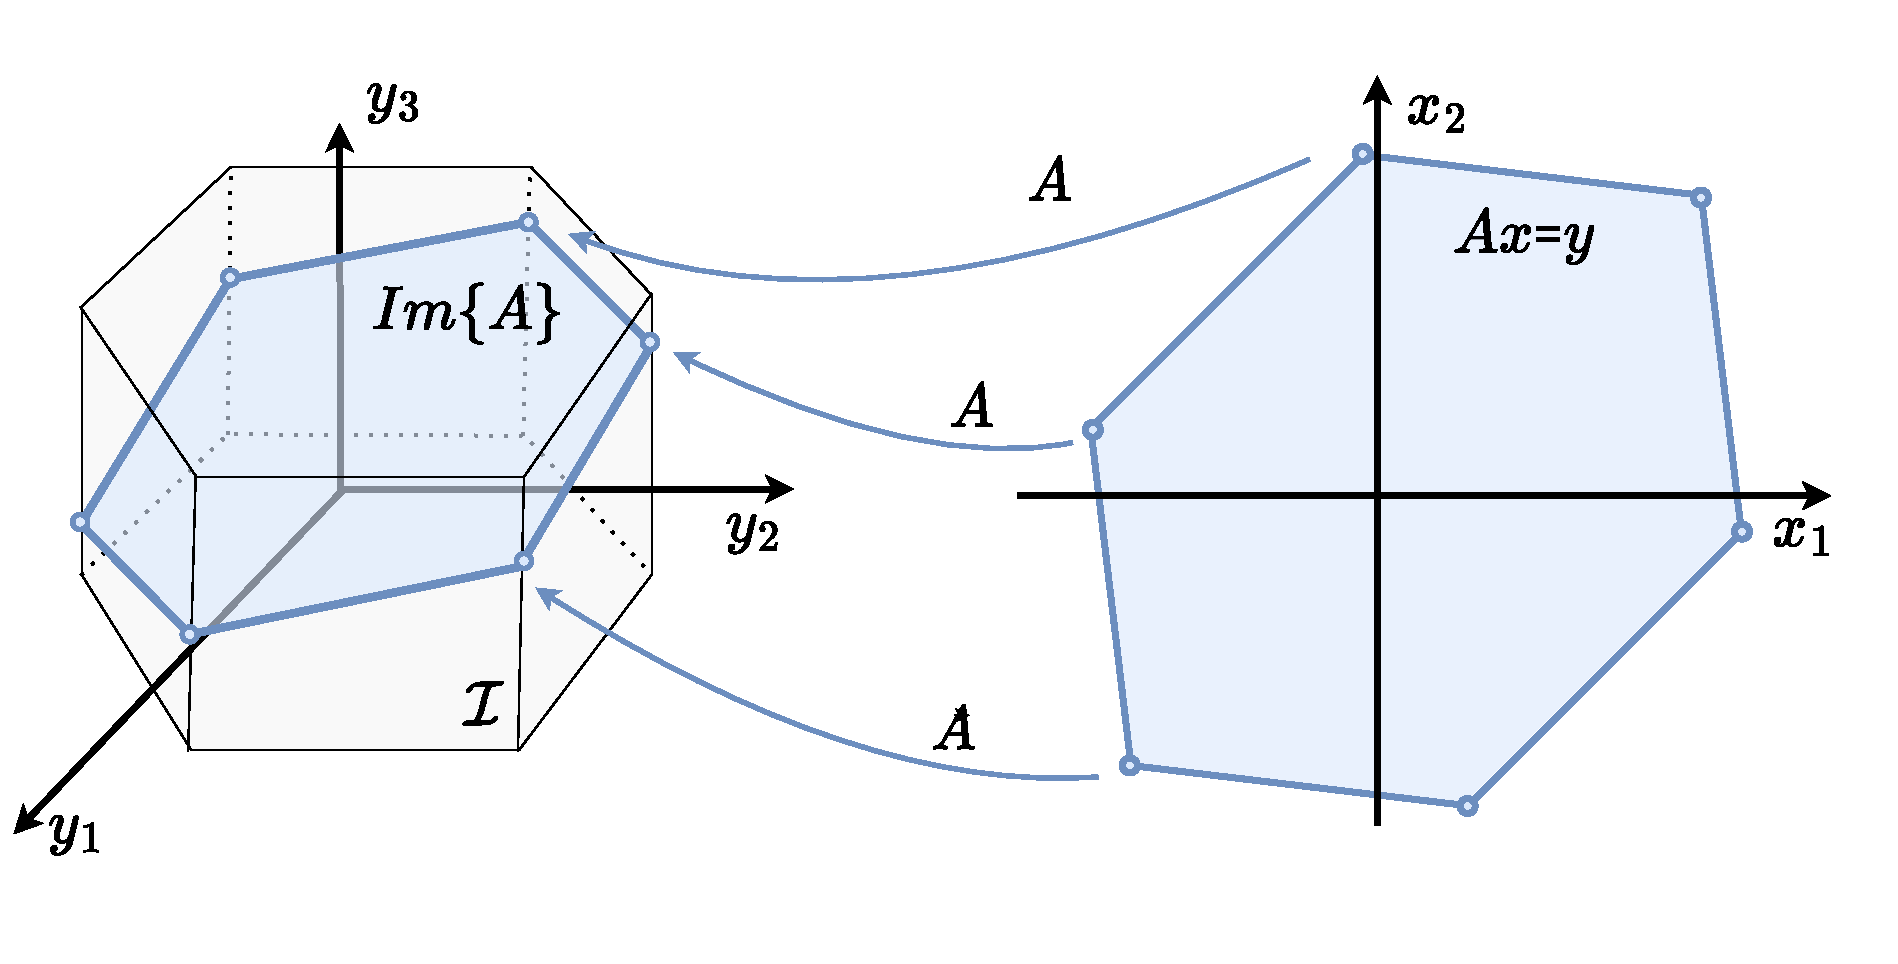
\includegraphics[width=0.8\linewidth]{Chapters/imgs/inter_poly.pdf}
    \caption{An example of the constructing an intersection formulation polytope with $m=2$ dimensional output space and $n=3$ dimensional input space. The input set $\mathcal{P}_y$ has a polytope form, and its intersection with the image of the matrix $A$ is shown in blue (left). The final polytope $\mathcal{P}_x$ is shown in blue as well (right).}
    \label{fig:inter_poly}
\end{figure}

The geometrical representation of the polytope $\mathcal{P}_x$ defined by (\ref{eq:inter_poly_revist}) is shown on Figure \ref{fig:inter_poly}, for the example of $n=3$ dimensional input set $\mathcal{P}_y$ and $m=2$ dimensional polytope $\mathcal{P}_x$. 
The resulting polytope $\mathcal{P}_x$ is an affine projection of the intersection of the input polytope $\mathcal{P}_y$ and the image $\img{A}$ of the matrix $A$ into the lower dimensional output space. As shown on Figure \ref{fig:inter_poly}, the vertices and faces of the polytope $\mathcal{P}_x$ do not correspond to the projection of the vertices and faces of the input polytope $\mathcal{P}_y$. 
Rather, as discussed in section \ref{par:equivalent_proj}, the polytope $\mathcal{P}_x$ is generated by projecting the intersection $\img{A}\cap\mathcal{P}_y$, of the polytope $\mathcal{P}_y$ and the image $\img{A}$ of the matrix $A$, to the output space. 
Therefore, there is a unique mapping between the vertices and faces of the intersection $\img{A}\cap\mathcal{P}_y$, and the vertices and the faces of the polytope $\mathcal{P}_x$, given through the pseudo-inverse inverse\cite{wang2018generalized} of the matrix $A$. 

Given the structure of the input set $\mathcal{P}_y$ algorithms for finding the $\repr{V}$ and $\repr{H}$-representation very in complexity. 

\subsubsection{Finding the $\repr{H}$-representation} 
\label{ch:inter_h_rep}
If the input set $\mathcal{P}_y$ is expressed in its $\repr{H}$-representation
\begin{equation}
    \mathcal{P}_y = \{ \bm{y}\in \mathbb{R}^n ~|~H_y\bm{y} \leq \bm{d}_y\}
\end{equation}
then finding the $\repr{H}$-representation of the polytope $\mathcal{P}_x$ is straightforward, by replacing the vector $\bm{y}$ with $A\bm{x} - \bm{b}_y$
\begin{equation}
    \mathcal{P}_x=\{\bm{x}\in  \mathbb{R}^m~|~ H_yA\bm{x} \leq \bm{d}_y -H_y\bm{b}_y \}
    \label{eq:inter_poly_h_rep}
\end{equation}
Even though this $\repr{H}$-representation (\ref{eq:inter_poly_h_rep}) of the polytope $\mathcal{P}_x$ follows directly from its definition and can be easily expressed, it might not be minimal. This means that even though the equation (\ref{eq:inter_poly_h_rep}) is correct and fully describes the polytope $\mathcal{P}_x$, there might be some redundant half-planes. Many algorithms have been developed over the years for removing the redundant half-planes equations \cite{Paulraj2006}, and their computational complexity is generally equivalent to solving a series of linear programming (LP) problems \cite{Telgen1983},\cite[Chapter 7.2]{fukuda2016lecture}. Therefore, depending on the application and the computational complexity of the polytope description necessary, such techniques can be used to reduce the equation (\ref{eq:inter_poly_h_rep}) to the minimal set of linear constraints.

However, if the polytope $\mathcal{P}_y$ is not expressed in $\repr{H}$-representation, in most cases the most efficient strategy is to first transform it to its $\repr{H}$-representation and the apply the manipulation described above. For example if the polytope $\mathcal{P}_y$ is expressed by its $\repr{V}$-representation, 
\begin{equation}
    \mathcal{P}_y = \conv{ \bm{y}_{v1}, ~ \bm{y}_{v2},~ \ldots}
\end{equation}
where $\bm{y}_{vi} \in \mathbb{R}^n$ are the vertices of $\mathcal{P}_y$.  These vertices can be transformed to the $\repr{H}$-representation using the techniques described in section \ref{ch:standard_represtantion_conversion}, which can then be used with the above described approach (\ref{eq:inter_poly_h_rep}) to obtain the $\repr{H}$-representation of the polytope $\mathcal{P}_x$.

Therefore, when it comes to finding the $\repr{H}$-representation of the polytope $\mathcal{P}_x$, the main complexity comes form determining the $\repr{H}$-representation of the input set $\mathcal{P}_y$. Where the input set $\mathcal{P}_y$, in general case, can have any formulation, not necessarily corresponding neither to the $\repr{V}$ nor to the $\repr{H}$-representation.

In this section three special cases of the input set formulation are discussed: intersection and projection formulation of the input set $\mathcal{P}_y$, as well as the interval form $\mathcal{I}_y$.

\paragraph*{Special case: intersection formulation} If the input set $\mathcal{P}_y$ has the intersection formulation itself
\begin{equation}
    \mathcal{P}_y=\{\bm{y}\in  \mathbb{R}^n~|~ C\bm{y}=\bm{z} + \bm{b}_z, ~ \bm{z} \in \mathcal{P}_z \}
\end{equation}
where $\bm{z}\in\mathcal{R}^k$ is a new its $k$ dimensional input vector, bounded within the set $\mathcal{P}_z$, $\bm{b}_z\in\mathbb{R}^k$ is the bias vector and the matrix $C\in \mathbb{R}^{k\times n}$ is a projector form the $n$ dimensional space to the $k$ dimensional space, where $k\geq n$.

Then the two intersection formulations can be combined into the new polytope $\mathcal{P}_x$, by replacing $\bm{y}$ with $A\bm{x}- \bm{b}_y$
\begin{equation}
    \mathcal{P}_x=\{\bm{x}\in  \mathbb{R}^m~|~ \underbrace{CA}_{A'}\bm{x}=\bm{z} + \underbrace{\bm{b}_z + C\bm{b}_y}_{\bm{b}_z'}, ~ \bm{z} \in \mathcal{P}_z \}
\end{equation}
which $\repr{H}$-representation can then be obtained in the same manner as described above.

\paragraph*{Special case: projection formulation} The common strategies for finding the $\repr{H}$-representation of polytopes with the projection formulation are described in the following section, section \ref{ch:projection_algos}.

\paragraph*{Special case: Interval form $\mathcal{I}_y$}  
\label{par:intersection_interval_algos_h}
\begin{figure}
    \centering
    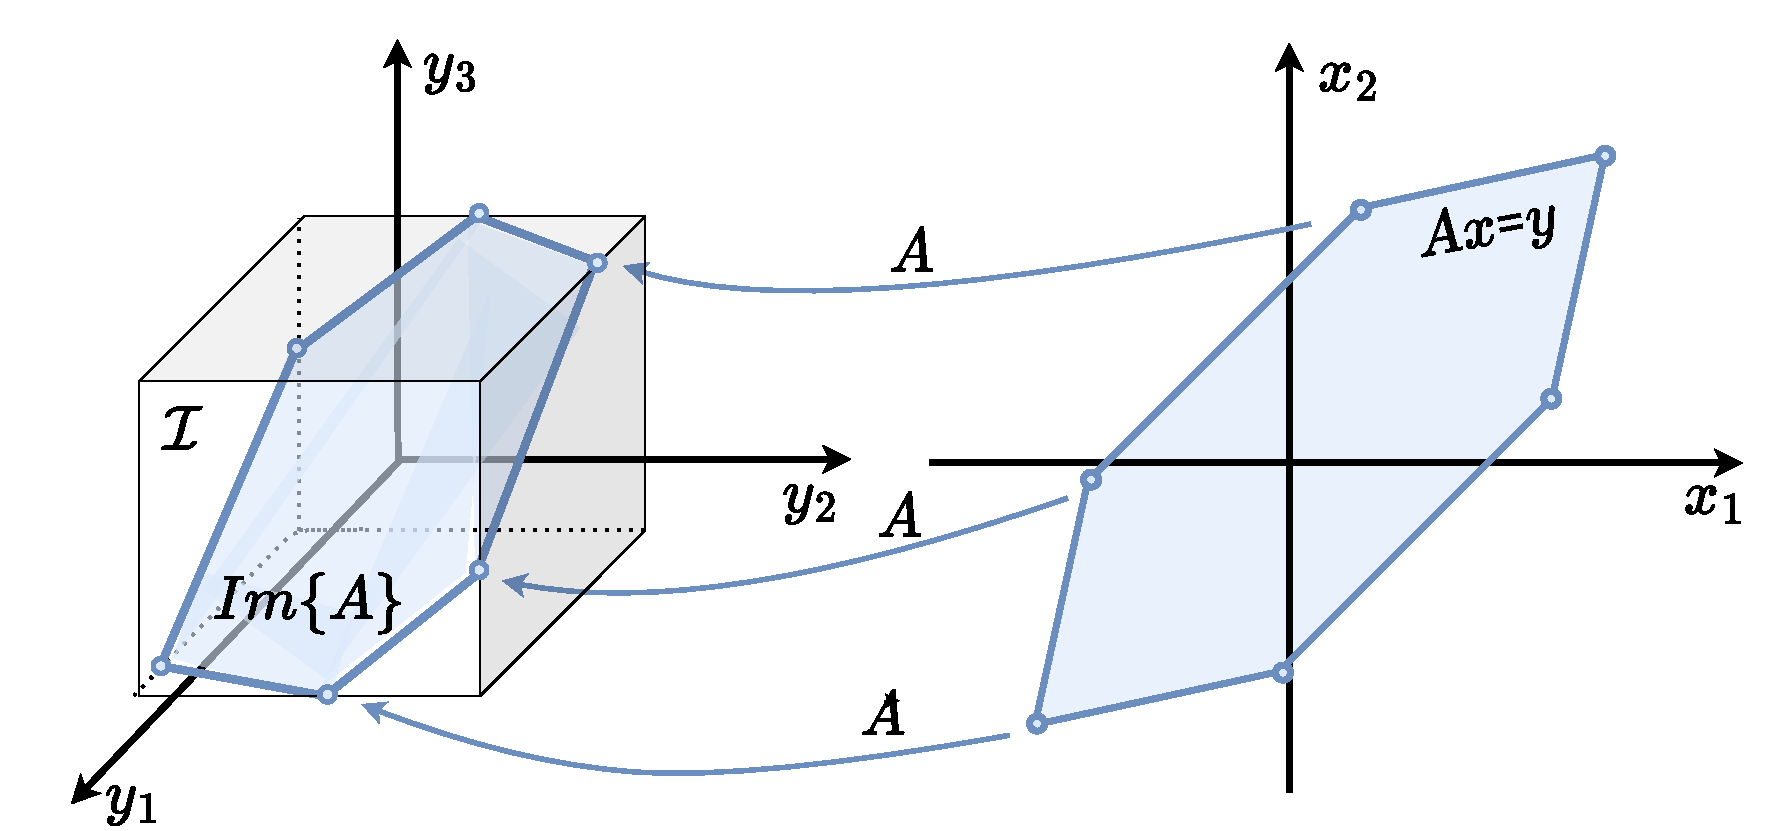
\includegraphics[width=0.8\linewidth]{Chapters/imgs/intersection.pdf}
    \caption{An example of the constructing an intersection formulation polytope with $m=2$ dimensional output space and $n=3$ dimensional input space. The intersection $\img{A} \cap \mathcal{I}_y$ of the hyperrectangle shaped input space $\mathcal{I}_y$ with the image of the matrix $A$ is shown in blue (left). This intersection can be projected to the output space using the inverse of the matrix $A$ to obtain the polytope $\mathcal{P}_x$ (blue right).}
    \label{fig:inter}
\end{figure}

The intersection polytope formulation (\ref{eq:inter_poly_revist}) with the interval limits 
\begin{equation}
    \mathcal{I}_y = \{ \bm{y}\in\mathbb{R}^n ~|~ \bm{y}\in[\bm{y}_{min},\bm{y}_{max}]\}
\end{equation}
is a spacial case of the intersection polytope formulation where the input space limits are defined as independent min-max ranges 
\begin{equation}
    \mathcal{P}_x=\{\bm{x}\in\mathbb{R}^m~ |~ A\bm{x} = \bm{y} + \bm{b}_y,~\bm{y}_{min} \leq  \bm{y} \leq \bm{y}_{max}  \}
    \label{eq:inter_hyp}
\end{equation}
Figure \ref{fig:inter} shows the graphical representation of constructing the polytope $\mathcal{P}_x$ from the input set $\mathcal{I}_y$.

When the input set has the interval form $\mathcal{I}_y$ the $\repr{H}$-representation of the polytope $\mathcal{P}_x$ can be found directly by substituting $\bm{y}$ with $A\bm{x}-\bm{b}_y$ in the interval equation $\bm{y}\in[\bm{y}_{min},\bm{y}_{max}]$ and rewriting it in the matrix from
\begin{equation}
   \underbrace{\begin{bmatrix}
        A\\
        -A
    \end{bmatrix}}_{H_x}\bm{x} \leq \underbrace{\begin{bmatrix}
         \bm{y}_{max} + \bm{b}_y\\
        -\bm{y}_{min} + \bm{b}_y 
    \end{bmatrix} }_{\bm{d}_x}
\end{equation}
where matrix $H_x\in\mathbb{R}^{2n \times m}$ and the vector $\bm{d}_x\in\mathbb{R}^{2n}$ can be used to express the $\repr{H}$-representation of the polytope $\mathcal{P}_x$
\begin{equation}
    \mathcal{P}_x=\{\bm{x}\in\mathbb{R}^m |~ H_x\bm{x} \leq \bm{d}_x \}
    \label{eq:inter_h_rep}
\end{equation}
However, as discusses above, additional steps might be necessary to remove the redundant hyper-plane equations within the matrix $H_x$ and the vector $\bm{d}_x$.


\subsubsection{Finding the $\repr{V}$-representation} 

Finding the $\repr{V}$-representation of polytopes with the intersection formulation, is much more complex operation with respect to finding the $\repr{H}$-representation. 

In general case, finding the $\repr{V}$-representation of the polytope $\mathcal{P}_x$, is performed by first finding its $\repr{H}$-representation, as described in in the previous section (section \ref{ch:inter_h_rep}). Then, depending on the size of the problem, different standard representation conversion algorithms, described in section \ref{ch:standard_represtantion_conversion}, can be used to obtain its $\repr{V}$-representation.

However, as the special case of the intersection formulation, where the input set has interval shape $\mathcal{I}_y$, is particularly present in the robotics literature, several efficient algorithms have been proposed for finding its $\repr{V}$-representation.



\paragraph*{Special case: Interval form $\mathcal{I}_y$}
\label{par:intersection_interval_algos_v}

When the input set has interval shape $\mathcal{I}_y$, the compact form of this polytope  $\mathcal{P}_x$ with the intersection formulation can be expressed as
\begin{equation}
    \mathcal{P}_x=\{\bm{x}\in\mathbb{R}^m ~ |~ A\bm{x} = \bm{y} + \bm{b}_y,~ \bm{y} \in [\bm{y}_{min},~  \bm{y}_{max}]  \}
    \label{eq:inter_hyp_revisit}
\end{equation}

Several efficient algorithms, particularly in robotics literature, were developed for finding all the vertices of the polytope $\mathcal{P}_x$. These algorithms, exploit the geometry of their respective problems and and provide better efficiency than the standard conversion INA or GTA based metods.

An efficient algorithm for vertex enumeration of the intersection type polytope is proposed by Gouttefarde et al. \cite{gouttefarde_versatile_2015}, exploiting the geometry of the problem and assuming that the output space dimension is always $m=2$, in which case the polytope $\mathcal{P}_x$ becomes a 2D polygon, which boundaries are then efficiently navigated in search for extremities. However, this algorithm does not scale well to higher dimensional problems.

A different algorithm, finding the $\repr{V}$-representation of the intersection polytope $\mathcal{P}_y$ with interval limits $\mathcal{I}_y$, is proposed by Chiacchio et al. \cite{chiacchio_evaluation_1996}. The algorithm leverages the hyperrectangle geometry of the interval input set $\mathcal{I}_y$ and performs an efficient exhaustive search through its faces. This algorithm has been improved by Sasaki et al. \cite{sasaki_vertex_nodate}, where the computational complexity has been significantly reduced by exploiting the geometry of the intersection of the hyperrectangle (interval) $\mathcal{I}_y$ and the image of matrix $\img{A}$, leveraging the equivalent projection formulation of the intersection polytope, described in the chapter \ref{par:equivalent_proj}.
\begin{equation}
\mathcal{P}_x=\{\bm{x}\in\mathbb{R}^m ~|~ \bm{x} = A^+\bm{y} + A^+\bm{b}_y,~ \bm{y} \in \img{A}\cap[\bm{y}_{min},\bm{y}_{max}]\}
\label{eq:inter_hyp_inter}
\end{equation}

Both of these algorithms Chiacchio et al. \cite{chiacchio_evaluation_1996} and Sasaki et al. \cite{sasaki_vertex_nodate} are based on the efficient exhaustive search of the hyperrectangle $\mathcal{I}_y$ faces. As the dimension of the input space $n$ grows the computational efficiency of these algorithms decreases, since the number of faces of the hypercube grows exponentially with the input space dimension
$$
N_{n,k}= 2^{n-k}\binom{n}{k}
$$
where $n$ is the dimension of the input space, $N_{n,k}$ is the number of the $k$ dimensional hyperrectangle faces.

\subsection{Strategies for projection formulation}
\label{ch:projection_algos}

This chapter brings a short overview of methods used for transformation of polytopes with projection formulation, described in chapter \ref{ch:proj_formulaiton}, into their respective $\repr{V}$ and $\repr{H}$-representation.

\label{ch:proj_poly_chapter}
\begin{figure}
    \centering
    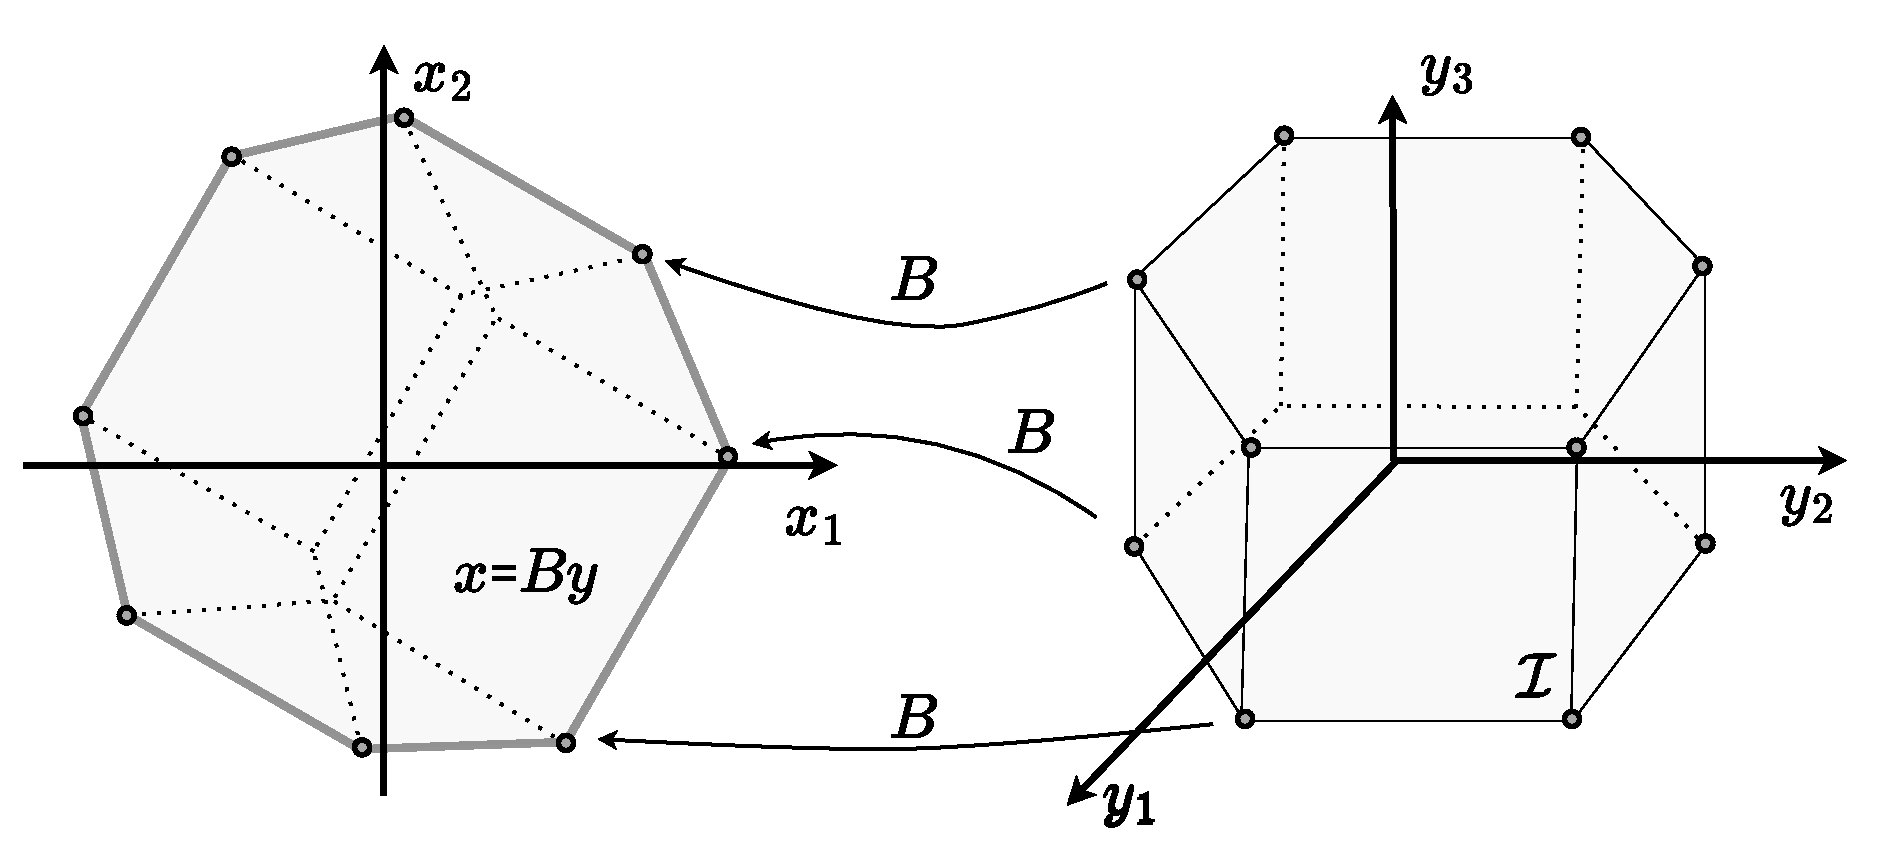
\includegraphics[width=0.7\linewidth]{Chapters/imgs/proj_poly.pdf}
    \caption{An example of the constructing a projection formulation polytope with $m=2$ dimensional output space and $n=3$ dimensional input space, where the input space $\mathcal{P}_y$ has a polytope shape. In this formulation, the whole input space $\mathcal{P}_y$ (grey) is projected using the matrix $B$ to the output space to obtain the polytope $\mathcal{P}_x$ (blue). }
    \label{fig:proj_poly}
\end{figure}

The projection polytope (\ref{eq:proj_poly}) with polytope input set $\mathcal{P}_y$ can be expressed as
\begin{equation}
    \mathcal{P}_x=\{\bm{x}\in\mathbb{R}^m |~ \bm{x} = B\bm{y} + \bm{b}_x,~\bm{y} \in \mathcal{P}_y  \}
    \label{eq:proj_poly_1}
\end{equation}
where $\bm{y}\in\mathbb{R}^n$ is an $n$ dimensional input vector, $\bm{x},\bm{b}_x\in\mathbb{R}^m$ are the $m$ dimensional output vector and bias, while $B\in\mathbb{R}^{n\times m}$ is a transformation matrix from input to the output space.

The geometrical representation of the polytope $\mathcal{P}_x$ defined by (\ref{eq:proj_poly_1}) is shown on Figure \ref{fig:proj_poly}, for the example of $n=3$ dimensional polytope $\mathcal{P}_y$ and $m=2$ dimensional polytope $\mathcal{P}_x$. The resulting polytope $\mathcal{P}_x$ is an affine projection of the polytope $\mathcal{P}_y$ into the lower dimensional output space. Furthermore, the vertices and the faces of the polytope $\mathcal{P}_x$ correspond to the subset of the projected vertices and faces of the polytope $\mathcal{P}_y$. 


Given the structure of the input set $\mathcal{P}_y$ algorithms for finding the $\repr{V}$ and $\repr{H}$-representation very in complexity. 

\subsubsection{Finding the $\repr{V}$-representation}
\label{ch:proj_algos_v}
If the input set polytope $\mathcal{P}_y$ is expressed using its vertex or $\repr{V}$-representation
\begin{equation}
    \mathcal{P}_y = \conv{ \bm{y}_{v1}, ~ \bm{y}_{v2},~ \ldots}
\end{equation}
where $\bm{y}_{vi}\in\mathbb{R}^n$ are the vertices of the polytope $\mathcal{P}_y$, the vertices of the projection formulation polytope (\ref{eq:proj_poly_1}) can then be found by projecting the vertices of $\mathcal{P}_y$ to the output space using the matrix $B \in \mathbb{R}^{m\times n}$ and calculating their convex-hull $\conv{\cdot}$
\begin{equation}
    \mathcal{P}_x= \conv{ B\bm{y}_{v1}, ~ B\bm{y}_{v2},~ \ldots}
\end{equation}
The convex-hull algorithm finds the $\repr{V}$-representation of the projection polytope directly, as the vertices of the polytope $\mathcal{P}_x$ are a subset of the projected vertices $\bm{y}_{vi}$ of the input polytope $\mathcal{P}_y$, as shown in the example on Figure \ref{fig:proj_poly}. 

If the input polytope $\mathcal{P}_y$ is expressed using its half-plane or $\repr{H}$-representation, 
\begin{equation}
    \mathcal{P}_y = \{ \bm{y}\in\mathbb{R}^n ~|~H_y\bm{y} \leq \bm{d}_y\}
\end{equation}
there are two main approaches decoupling the problem.

The first and straight-forward approach consists in finding the $\repr{V}$-representation of the input set $\mathcal{P}_y$ first, using the standard representation conversion methods described in section \ref{ch:standard_represtantion_conversion}, then follow the above described procedure to find the desired representation of the $\mathcal{P}_x$. However, in many cases, when the input space dimension $n$ is high or if the geometry of the polytope  $\mathcal{P}_y$ is complex (large number of faces and vertices), finding its $\repr{V}$-representation might be computationally demanding. 

The second approach, that is more efficient in many cases, consists in finding the $\repr{H}$-representation of the polytope $\mathcal{P}_x$ directly from the input set's $\repr{H}$-representation. One of the most well known algorithm fro projecting the $\repr{H}$-representation of polytopes is arguably Fourier-Motzkin Elimination (FME) described by Dantzig and Eaves \cite{dantzig1973fourier}.  This algorithm uses an iterative inequality elimination method to isolate the set of half-plane equations bounding the final polytope $\mathcal{P}_x$. However, this approach has an exponential complexity with the dimension of the input space $n$ \cite{Talaashrafi2020complexity}, and additionally it does not guarantee minimal representation \cite{Monniaux2010}. A more efficient algorithms is introduced by Jones et al. called Equality-Set Projection \cite{jones2004equality}. As opposed to FME, this algorithm is \textit{output sensitive}, having the execution time proportional to the complexity of the final polytope $\mathcal{P}_x$ (it number of faces and vertices), making it particularly well suited to the high dimensional input spaces $\mathbb{R}^n$. A more in depth comparison of these methods, as well their comparison to several other polytope projection algorithms, is brought in the work by Glassle et al. \cite{Gl_le_2018}. Once the $\repr{H}$-representation of the polytope $\mathcal{P}_x$ is obtained using one of these methods, Then, the standard representation conversion methods can be used to obtain the $\repr{V}$-representation of the polytope $\mathcal{P}_x$ defined in the $m$ dimensional output space.

These same two approaches can be used in the general case, where the input set $\mathcal{P}_y$ does not correspond neither to the $\repr{V}$ not to the $\repr{H}$-representation. The choice of the more suitable one depends on the efficiency of transforming the input set $\mathcal{P}_y$ into its $\repr{V}$ or $\repr{H}$-representation. 

In this section three special cases of the input set formulation are discussed: intersection and projection formulation of the input set $\mathcal{P}_y$, as well as the interval form $\mathcal{I}_y$.

\paragraph*{Special case: intersection formulation} If the input set $\mathcal{P}_y$ has the intersection formulation, then its $\repr{H}$ and $\repr{V}$-representations can be obtained using the strategies discussed in section \ref{ch:intersection_algos}. When it comes to the input sets $\mathcal{P}_y$ with intersection formulations,  their $\repr{H}$-representations can be obtained directly from their definitions, while finding their $\repr{V}$-representations is more computationally demeaning operation.

\paragraph*{Special case: projection formulation} 
If the input set $\mathcal{P}_y$ has the projection formulation itself
\begin{equation}
    \mathcal{P}_y=\{\bm{y}\in  \mathbb{R}^n~|~ \bm{y}=D\bm{z} + \bm{b}_y, ~ \bm{z} \in \mathcal{P}_z \}
\end{equation}
where $\bm{z}\in\mathcal{R}^k$ is a new its $k$ dimensional input vector, bounded within the set $\mathcal{P}_z$, $\bm{b}_y\in\mathbb{R}^n$ is the bias vector, and the matrix $D\in \mathbb{R}^{n\times k}$ is a projector form the $k$ dimensional space to the $n$ dimensional space, where $k\geq n$.

Then the two projection formulations can be combined into the new polytope $\mathcal{P}_x$, by replacing the $\bm{y}$ with $D\bm{z} + \bm{b}_y$ in initial formulation of $\mathcal{P}_x$ (\ref{eq:proj_poly_1}).
\begin{equation}
    \mathcal{P}_x=\{\bm{x}\in  \mathbb{R}^m~|~ \bm{x}=\underbrace{BD}_{B'}\bm{z} + \underbrace{B\bm{b}_z + \bm{b}_x}_{\bm{b}_x'}, ~ \bm{z} \in \mathcal{P}_z \}
\end{equation}
which $\repr{V}$-representation can be found in the same manner as described above.

\paragraph*{Special case: Interval form $\mathcal{I}_y$} 


\begin{figure}
    \centering
    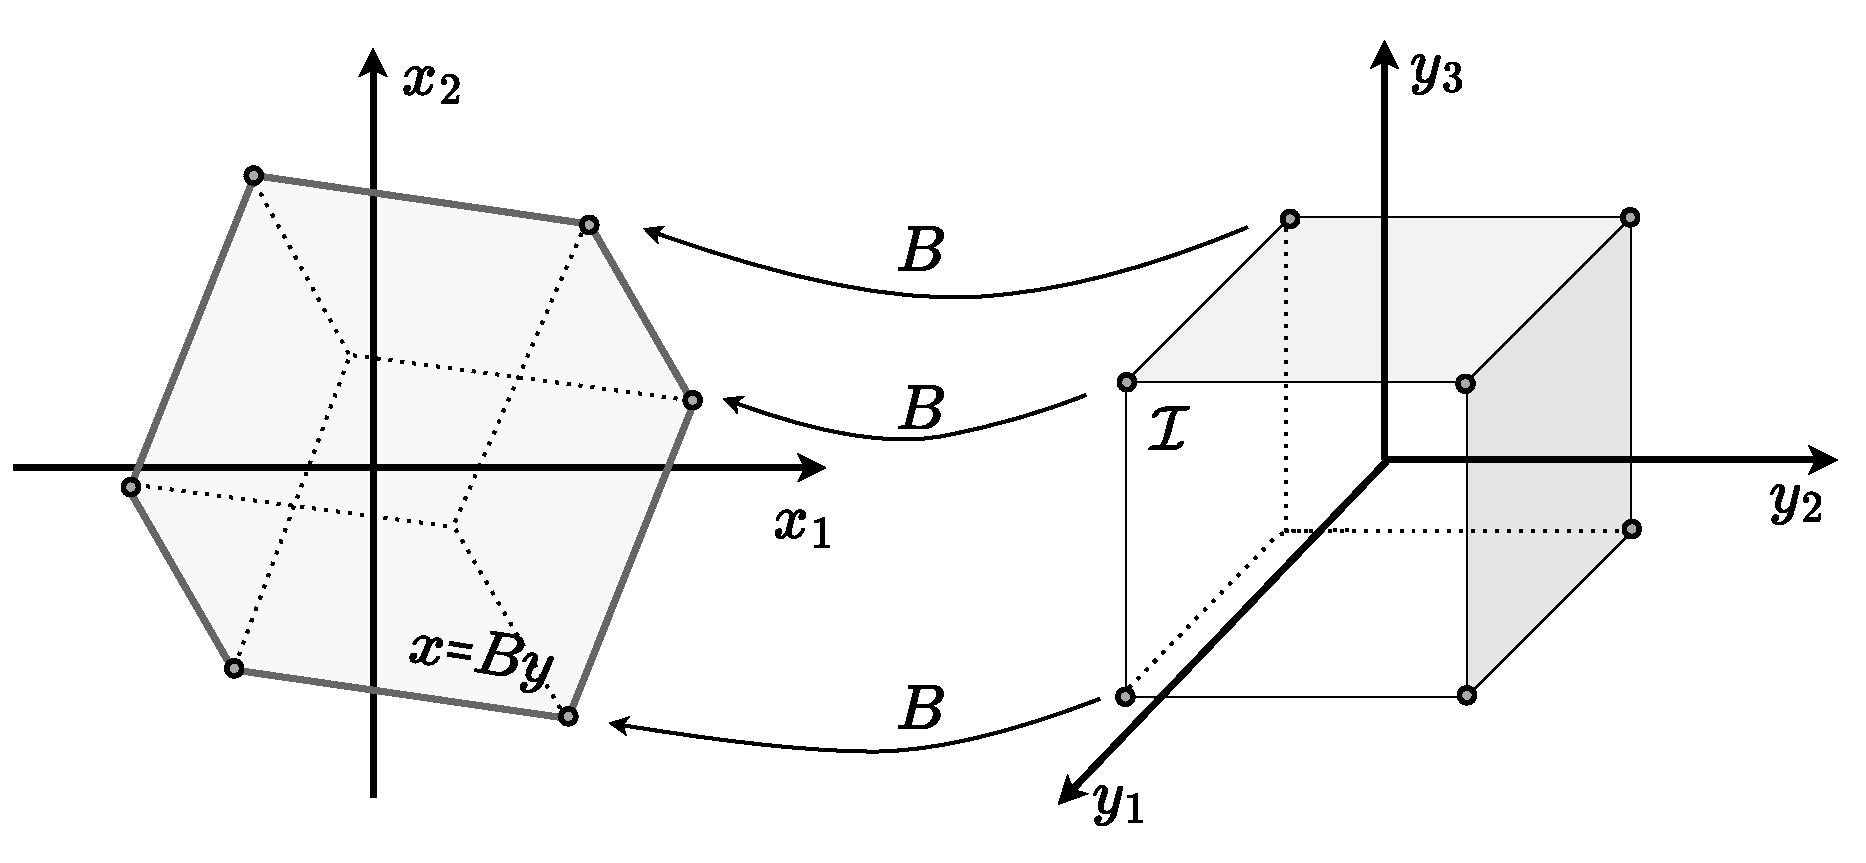
\includegraphics[width=0.8\linewidth]{Chapters/imgs/projection.pdf}
    \caption{An example of the constructing a projection formulation polytope with $m=2$ dimensional output space and $n=3$ dimensional input space, where the input space $\mathcal{I}_y$ has a hyperrectangle (interval) shape. In the projection formulation, the whole input space $\mathcal{I}_y$ (grey) is projected using the matrix $B$ to the output space to obtain the polytope $\mathcal{P}_x$ (blue). }
    \label{fig:proj}
\end{figure}

The projection polytope formulation $\mathcal{P}_x$ with the interval limits $\mathcal{I}_y$
\begin{equation}
    \mathcal{I}_y = \{ \bm{y}\in\mathbb{R}^n ~|~ \bm{y}\in[\bm{y}_{min},\bm{y}_{max}]\}
\end{equation}
is a spacial case of the projection polytope formulation which can be compactly expresses as
\begin{equation}
    \mathcal{P}_x=\{\bm{x}\in\mathbb{R}^m |~ \bm{x} = B\bm{y} + \bm{b}_x,~\bm{y}_{min} \leq  \bm{y} \leq \bm{y}_{max}  \}
    \label{eq:proj_hyp}
\end{equation}
Figure \ref{fig:proj} shows the graphical representation of constructing the polytope $\mathcal{P}_x$ from the input set $\mathcal{I}_y$.

The most straight-forward way of finding the vertices $\bm{x}_{vi}\in\mathbb{R}^m$ of the projection polytope $\mathcal{P}_x$ is by first enumerating the $2^n$ vertices $\bm{y}_{vi}\in\mathbb{R}^n$ of the hyperrectangle  (interval) $\mathcal{I}_y$, by creating a list of all the combinations of the minimal $\bm{y}_{min}$ and maximal $\bm{y}_{max}$ values of $\bm{y}$
\begin{equation}
    \bm{y}_{v1} = \begin{bmatrix}
        y_{1,min}\\
        y_{2,min}\\
        \ldots\\
        y_{n,min}\\
    \end{bmatrix},\quad
    \bm{y}_{v2} = \begin{bmatrix}
        y_{1,max}\\
        y_{2,min}\\
        \ldots\\
        y_{n,min}\\
    \end{bmatrix},\qquad\ldots,\qquad
    \bm{y}_{v2^n} = \begin{bmatrix}
        y_{1,max}\\
        y_{2,max}\\
        \ldots\\
        y_{n,max}\\
    \end{bmatrix} 
\end{equation}
Then these vertices can be projected to the lower dimensional output space $\mathbb{R}^m$ using the projection matrix $B\in \mathbb{R}^{m\times n}$, where the polytope $\mathcal{P}_x$ can be found by calculating the convex-hull $\conv{\cdot}$ of the projected points.
\begin{equation}
    \mathcal{P}_x = \conv{B\bm{y}_{v1},B\bm{y}_{v2},~\ldots, ~ B\bm{y}_{v2^n}}
\end{equation}

The complexity of this approach depends on two factors. The dimension of the of the input space $n$ and the dimension of the output space $m$. The number of vertices of the hyperrectangle (interval) is grows exponentially $2^n$ with the dimension of the input space $n$, and constructing a matrix of $2^n \times n$ entries can become impractical. On the other hand, as this approach requires a convex-hull algorithms, which are executed in the $m$-dimensional output space, the dimension $m$ might make the convex-hull algorithm impractical as their complexity grows significantly with the dimension of the space $m$ \cite{Barber1996}.

Therefore for higher dimensional output spaces (typically $m> 4$) and output spaces (causing the memory issues due to  $2^n \times n$ matrix construction) a more efficient approach might be to first calculate the $\repr{H}$-representation of this polytope, using the methods described in the following section, and then use standard representation conversion methods (section \ref{ch:standard_represtantion_conversion}), to find its $\repr{V}$-representation.


\subsubsection{Finding the $\repr{H}$-representation}
\label{ch:proj_algos_h}

If the input polytope $\mathcal{P}_y$ is expressed using its half-plane or $\repr{H}$-representation, 
\begin{equation}
    \mathcal{P}_y = \{ \bm{y}\in\mathbb{R}^n ~|~H_y\bm{y} \leq \bm{d}_y\}
\end{equation}
the straight-forward approach consists in decoupling the problem and find the $\repr{V}$-representation first, using the standard representation conversion methods  described in section \ref{ch:standard_represtantion_conversion}, then follow the above described procedure to find the desired representation of the $\mathcal{P}_x$. 

As described in the previous section, in many cases, when the input space dimension $n$ is high or if the geometry of the polytope  $\mathcal{P}_y$ is complex (large number of faces and vertices), finding its $\repr{V}$-representation might be computationally demanding. In those cases, if the $\repr{H}$-representation of the polytope $\mathcal{P}_y$ is available, the $\repr{H}$-representation of the polytope $\mathcal{P}_x$ can be found directly using the algorithms such as Fourier-Motzkin Elimination (FME) and Equality-Set Projection (ESP). 

These same two approaches can be used in the general case, where the input set $\mathcal{P}_y$ does not correspond neither to the $\repr{V}$ not to the $\repr{H}$-representation. The choice of the more suitable one depends on the efficiency of transforming the input set $\mathcal{P}_y$ into its $\repr{V}$ or $\repr{H}$-representation. 


\paragraph*{Special case: Interval form $\mathcal{I}_y$} 

The projection polytope formulation $\mathcal{P}_x$ with the interval limits $\mathcal{I}_y$ can be compactly expresses as
\begin{equation}
    \mathcal{P}_x=\{\bm{x}\in\mathbb{R}^m |~ \bm{x} = B\bm{y} + \bm{b}_x,~\bm{y}_{min} \leq  \bm{y} \leq \bm{y}_{max}  \}
    \label{eq:proj_hyp_1}
\end{equation}

Apart from the two approaches described earlier, that are applicable to this polytope formulation (\ref{eq:proj_hyp_1}) as well, there are several more efficient algorithms introduced in the literature specific for this formulation, typically exploiting the polytope's Zonotope structure.

One such  efficient algorithm, exploiting the geometry of the formulation (\ref{eq:proj_hyp_1}) of projection polytope $\mathcal{P}_x$ with interval limits $\mathcal{I}_y$, is introduced by Bouchard et al. \cite{Bouchard2009} and improved by Gouttefarde and Krut \cite{hyper_psm}, called Hyper-Plane Shifting Method (HPSM). This algorithm finds the minimal $\repr{H}$-representation of the polytope (\ref{eq:proj_hyp_1}) by efficiently performing the exhaustive search of all the possible half-plane combinations corresponding to the $m-1$ dimensional polytope $\mathcal{P}_x$ faces. Even-though much more efficient than the Fourier-Motzkin elimination, this algorithm still has considerable (binomial) complexity, as it relies on the exhaustive search in the $n$ dimensional input space where the number $N_h$ of hyper-planes to be tested equals to 
$$N_h = \binom{n}{m-1}$$

\subsection{Polytope approximation strategies}
\label{ch:approximation_algos}

Exact vertex and facet enumeration methods, such the standard representation conversion methods described in section \ref{ch:standard_represtantion_conversion} or more specific methods for the projection and the intersection formulation described in \ref{ch:intersection_algos} and \ref{ch:projection_algos}, rely on different versions of exhaustive search in the $n$-dimensional input space, which is often higher dimensional than the output space $n> m$. Their execution time is typically exponential, or polynomial in the best case, with respect to the dimension of the input space $n$, the number of vertices and the faces of the input set $\mathcal{P}_y$ and the final polytope $\mathcal{P}_x$ \cite{Dyer1983}. Therefore, in cases where the input space is much higher dimensional than output space $n\gg m$ or when the polytopes $\mathcal{P}_x$ and $\mathcal{P}_y$ have complex geometries (large number of faces and vertices), such approaches may not be practically viable for interactive, in-the-loop, applications. 

\begin{wrapfigure}{r}{0.35\linewidth}
    \centering
    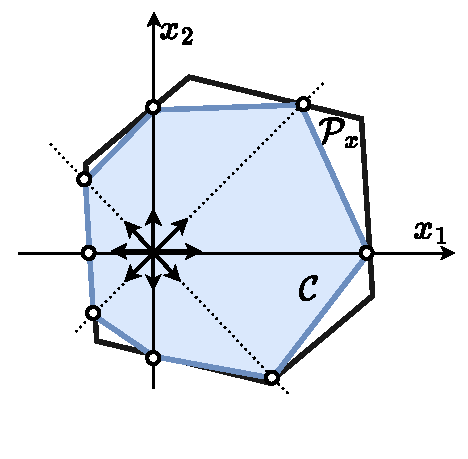
\includegraphics[width=\linewidth]{Papers/images/rsm.pdf}
    \caption{An example of the approximation $\mathcal{C}$ of the 2D ($m\!=\!2$) polytope $\mathcal{P}_x$ using a RSM algorithm. The input space is sampled with 8 rays. }
    \label{fig:rsm}
\end{wrapfigure}
To overcome this issue, various approximate approaches, such as the  \textit{Ray Shooting Method} (RSM)  \cite{agarwal1993ray} and the \textit{Convex-Hull Method} (CHM) \cite{lassez1992quantifier}, have been developed, reducing the complexity and improving the execution time. 


The RSM algorithms are relatively simple to setup as they rely on different forms of sampling (shooting rays) of the polytope $\mathcal{P}_x$, in the low dimensional output space. Their execution time is proportional to the number of sampling directions (rays shot), therefore by choosing an appropriate sampling strategy the RSM algorithms can provide an efficient approximation of the polytope $\mathcal{P}_x$. However, these algorithms do not provide any bound on their estimation error and rely highly on hand tuned initial parameters. Figure \ref{fig:rsm} shows a visual example of a RSM approximation of a polygon $\mathcal{P}_x$ using uniform sampling in the output space with 8 rays.

The CHM algorithms, first introduced by Lassez et al. \cite{lassez1992quantifier, Huynh2005PracticalIO}, propose an efficient iterative approximation of the polytope $\mathcal{P}_x$, while at the same time avoiding the complexity of the exhaustive search and simplifying the final polytope $\mathcal{P}_x$ geometry by removing the need to find all the faces and vertices of the polytope. Such algorithms are usually defined in the lower-dimensional output space $\bm{x}\in \mathbb{R}^m$ making them \textit{output sensitive}, having the execution time proportional to the number of vertices and the faces of the output space polytope $\mathcal{P}_x$. In addition to searching in the lower $m$ dimensional output space, they enable finding an efficient inner (or outer) approximation of the polytope $\mathcal{P}_x$, while satisfying different measures of the approximation accuracy. Finally, they find both the vertices and the faces of the polytope $\mathcal{P}_x$ at the same time, providing both $\repr{V}$ and $\repr{H}$-representation \cite{Gl_le_2018}.


The execution of typical CHM algorithm consists in two phases. In the first phase an initial approximation of the polytope $\mathcal{P}_x$ is constructed finding a subset of $m+1$ vertices forming an initial $m$-dimensional convex-hull $\mathcal{C}$ approximation of the polytope $\mathcal{P}_x$. In the second phase, the convex-hull approximation $\mathcal{C}$ is refined iteratively until the desired accuracy is reached. The CHM algorithms use a sequence of linear programs (LP) to find new vertices of the polytope in each iteration, followed by the convex-hull algorithm to group them to the faces. An example of the CHM algorithm iterations in for $m=2$ output space is shown on Figure \ref{fig:chm}.   

The CHM algorithms have several limitations though. The resolution of the algorithms relies on the iterative application of the convex-hull algorithm which complexity grows exponentially for output space dimensions $m > 3$ \cite{Barber1996}. As a result, the applications of these methods have so far been limited to the low-dimensional output spaces $m\leq3$. Additionally, as different polytope formulations require different LP formulations, the implementations of these methods are often somewhat specific to their respective applications. 

There are several examples in the literature where the approximation based methods were used for improving the efficiency of different computationally expensive polytope evaluation problems. Bretl et al. \cite{Bretl2008} have proposed a CHM based algorithm for approximating 2D ($m\!=\!2$) polytopes in the context of legged robot locomotion. Del Prete el al. \cite{DelPrete2016Fast} recently proposed an efficiency improvement of this algorithm, and Audren et al. \cite{Herve2018} extended it to the 3D ($m\!=\!3$) use-cases. This algorithm calculates the inner and outer approximation of the polytope $\mathcal{P}_x$ at the same time, while its accuracy condition can be set a as desired ratio between the inner and outer approximation volumes. Ponce and Faverjon \cite{Ponce1995} have introduced a derivative of the CHM algorithm to calculate the 2D, 3D and 4D ($m\!=\!2,3,4$) polytopes in the context of grasping objects with multiple fingers. While Xu et al. \cite{Xu2008projection} used a CHM algorithm in the context in the context of information theory. Both of these algorithms find all vertices and faces of the output polytope $\mathcal{P}_x$, without exploiting CHM's approximation capacity. Furthermore, Carmicahel et al. \cite{carmichael_estimating_2013,carmichael2011Towards} used an RSM algorithm for approximating 2D and 3D ($m\! =\! 2,3$) polytopes in the context of human force capacity estimation, based on his musculoskeletal model. In order to enable real-time execution, their RSM implementation relies on the uniform sampling in the output space.

 
\begin{figure}
    \centering
    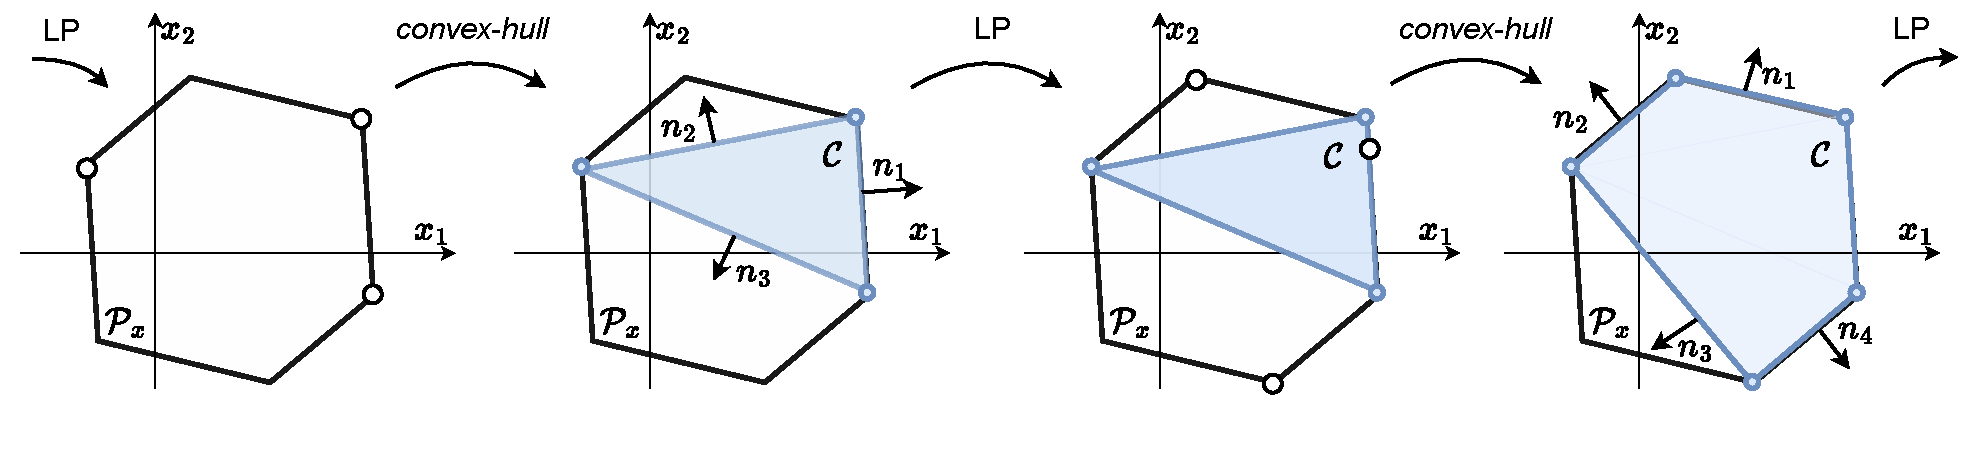
\includegraphics[width=\linewidth]{Papers/images/chm_algo.pdf}
    \caption{This figure shows the procedure of successive approximation of the polytope $\mathcal{P}_x$ using the CHM algorithm. The face normal vectors $\bm{n}_i$ of the convex-hull $\mathcal{C}$ are used with Linear programming (LP) to find new vertices which are then used to update the convex-hull $\mathcal{C}$ and furthermore improve the approximation of the polytope.}
    \label{fig:chm}
\end{figure}

In summary, when the the complexity of the polytope $\mathcal{P}_x$ transformation does not permit using standard exact methods in the practical applications, especially when the dimension $n$ of the input space is high while the dimension of the output space $m$ is reasonably low $m\leq3$, polytope approximation methods, such as RSM and CHM algorithms, provide a more efficient solutions. The RSM algorithms provide a fast sampling based approximation, however without any guarantees on the approximation error or accuracy. On the other hand, CHM algorithms use an efficient iterative approach to the polytope approximation, while at the same time being capable of guaranteeing the maximal approximation error.

\section{New vertex finding algorithm for intersection formulation}
\label{sec:algorithm_vea}

One typical example of the polytope with the intersection formulation (\ref{eq:inter_poly}) and interval input set (\ref{eq:hypercube_lim}) is the feasible wrench polytope, discussed in section \ref{ch:poly_force},
\begin{equation}
    \mathcal{P}_f(\bm{q},\dot{\bm{q}},\ddot{\bm{q}}) = \left\{ \bm{f} \in \mathbb{R}^m ~|~ \bm{\tau}\in\left[\bm{\tau}_{min}, \bm{\tau}_{max} \right], ~~ J^T(\bm{q})\bm{f} = \bm{\tau} -\bm{\tau}_b(\bm{q},\dot{\bm{q}},\ddot{\bm{q}}) \right\}
    \label{eq:poly_force_rob_revisit_algo}
\end{equation}
where the input space corresponds to the space of applicable joint torques $\bm{\tau}\in\mathbb{R}^n$, the output space is the set feasible cartesian wrenches (forces) $\bm{f}\in\mathbb{R}^m$ and the mapping between the two is given through the jacobian transpose matrix $J(\bm{q})^T\in\mathbb{R}^{n\times m}$. Additionally, the bias vector $\bm{\tau}_b$ groups the influences of robot's motion and gravity.

Being able to characterise the robot's wrench generation capacity exactly, as in the case of the polytope \ref{eq:poly_force_rob_revisit_algo}, has a potential to enable more adapted robot control strategies leveraging this fine information about robot's true capacity.  As the polytope $\mathcal{P}_f$ is state dependant, its shape and the size vary significantly with respect to the robot's state $\{\bm{q},\dot{\bm{q}}\}$ and potentially desired acceleration $\ddot{\bm{q}}$ to be achieved. Therefore, when it comes to using the polytope $\mathcal{P}_f$ in real-time robot control applications, where the robot exchanges wrenches with different objects and tools in the environment, or even with human operators, in order to ensure that the robot is capable of generating the wrenches in question, the wrench polytope $\mathcal{P}_f$ has to be evaluated in real-time too. 

Typical robot control strategies require the cycle times in the range of a few milliseconds in order to ensure satisfactory results. Therefore, to integrate the wrench polytopes $\mathcal{P}_f$ in the robot control applications, these polytope $\mathcal{P}_f$ need to be transformed to a suitable representation ($\repr{H}$ or $\repr{V}$) in comparable times as well.


In a generic form this robot's wrench capacity polytope $\mathcal{P}_x$ can be expressed as
\begin{equation}
    \mathcal{P}_x=\{\bm{x}\in\mathbb{R}^m~ |~\bm{y}\in[\bm{y}_{min}, \bm{y}_{max}], ~ A\bm{x} = \bm{y}\}
    \label{eq:inter_hyp_revisit_algo}
\end{equation}
where the matrix $A\in\mathbb{R}^{n\times m}$ corresponds to the jacobian transpose $J(\bm{q})^T$ and $\bm{x}\in\mathbb{R}^m$ corresponds to the cartesian wrench $\bm{f}$, while $\bm{y}\in\mathbb{R}^n$, without the loss of generality, corresponds to the achievable joint torques $\bm{\tau}$ reduced by the fixed bias $\bm{\tau} - \bm{\tau}_b$.  Additionally, the input set can be expressed in the interval form
\begin{equation}
    \mathcal{I}_y=\{\bm{y}\in\mathbb{R}^n~ |~\bm{y}\in[\bm{y}_{min}, \bm{y}_{max}]~\}
    \label{eq:interval_revisit_algo}
\end{equation}

As discussed in section \ref{par:intersection_interval_algos_h}, the $\repr{H}$-representation of the intersection formulation based polytopes comes directly from their definition and is easy to obtain, therefore in this section the accent is put on transforming the polytope $\mathcal{P}_f$ to its $\repr{V}$ representation. As discussed in section \ref{par:intersection_interval_algos_v}, there are several algorithms introduced in the literature that enable efficient vertex enumeration of intersection polytopes $\mathcal{P}_x$  with interval input set $\mathcal{I}_y$. Two of such examples are the algorithms introduced by Chiacchio et al.~\cite{chiacchio_evaluation_1996} and Sasaki et al.~\cite{sasaki2011vertex}.

In this section, a new algorithm for efficient finding the $\repr{V}$-representation of this polytope formulation is presented, building upon the findings form the algorithm proposed by Sasaki et al. The proposed algorithm reduces the complexity of the exhaustive search for the vertices of the polytope $\mathcal{P}_x$ by exploiting the geometry of the problem. The algorithm is compared, section \ref{sec:complexity}, with the the state of the art algorithms from Chiacchio et al. and Sasaki et al. and shown to have lower complexity and shorter execution time. Furthermore, the results show that the proposed algorithm is capable of finding $\repr{V}$-representation of this family of polytopes within a few milliseconds, for problem sizes corresponding to those in evaluating the wrench capacity (\ref{eq:poly_force_rob_revisit_algo}) of standard robotic manipulators, opening doors for potential applications in real-time applications.


\subsection{Problem definition}

\begin{figure}[!h]
    \centering
    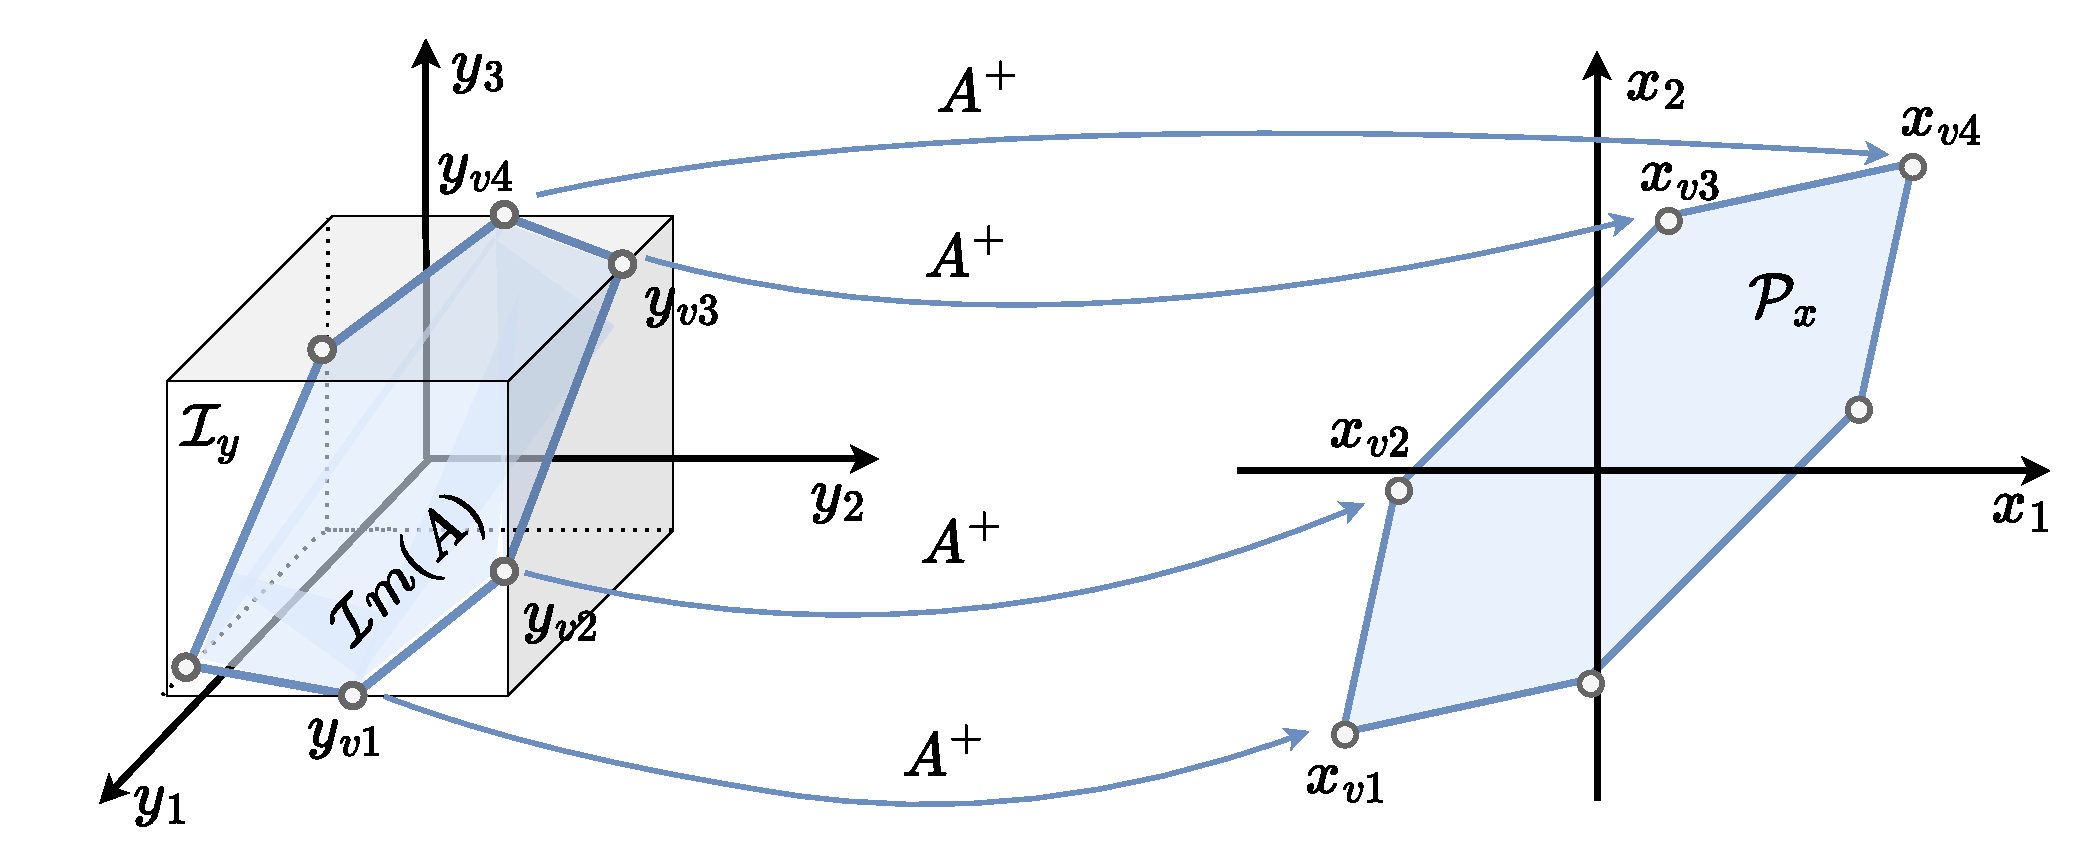
\includegraphics[width=0.8\linewidth]{Papers/images/intersection_algo.pdf}
    \caption{Example intersection polytope $\mathcal{P}_x$ with $n=3$ dimensional interval input set $\mathcal{I}_y$ and $m=2$ dimensional output space. The polytope $\mathcal{P}_x$ vertices $\bm{x}_{vi}$ correspond to the vertices of the intersection $\mathcal{I}_y\cap\img{A}$ denoted as $\bm{y}_{vi}$, through the pseudo-inverse $A^T$ of the matrix $A$.}
    \label{fig:intersection_algo}
\end{figure}

As shown on Figure \ref{fig:intersection_algo}, the space of all the input vectors $\bm{y}\in\mathbb{R}^n$, bounded within the interval shaped input set $\mathcal{I}_y$, geometrically forms an $n$-dimensional hyperrectangle (orhtotope) with $n$ pairs of parallel sides defined by the output limits $\bm{y}\in[\bm{y}_{min}\bm{y}_{max}]$. The image of the $A$ matrix $\img{A}$ is a $r$-dimensional subspace of the hyperrectangle, where $r$ is the rank of $A$. In  the remainder of this section, the matrix $A$ is, without loss of generality, assumed to be in not singular $m$=$r$. 

As discussed in section \ref{ch:inter_formulaiton}, the output space polytope $\mathcal{P}_x$ is the direct affine projection of the intersection between the image $\img{A}$ and the input set $\mathcal{I}_y$ using the pseudo-inverse $A^+$ of the matrix $A$. Therefore this algorithm aims to efficiently find the vertices $\bm{x}_{v}$ of the polytope $\mathcal{P}_x$, by efficiently finding the vertices $\bm{y}_{v}$ of the intersection $\mathcal{I}\cap \img{A}$, and project them to the output space using the relationship
\begin{equation}
    \bm{x}_v = A^{+}\bm{y}_v, \qquad \text{where} \quad \bm{y}_v\in\mathcal{I}_y\cap \img{A} \label{eq:compute_vert}
\end{equation}

Therefore the operation of enumerating all the vertices $\bm{x}_{v}$ of the polytope $\mathcal{P}_x$ can be seen as first finding the $\repr{V}$-representation (the set of vertices $\bm{y}_{v}$) of the intersection  $\mathcal{I}\cap \img{A}$, followed by its projection to the output space through the pseudo-inverse $A^+$, to obtain the $\repr{V}$-representation of the polytope $\mathcal{P}_x$
\begin{equation}
    \mathcal{P}_x = \conv{A^+\bm{y}_{v1},~A^+\bm{y}_{v1},~\ldots~ }
\end{equation}


\begin{wrapfigure}{r}{0.5\linewidth}
    \centering
    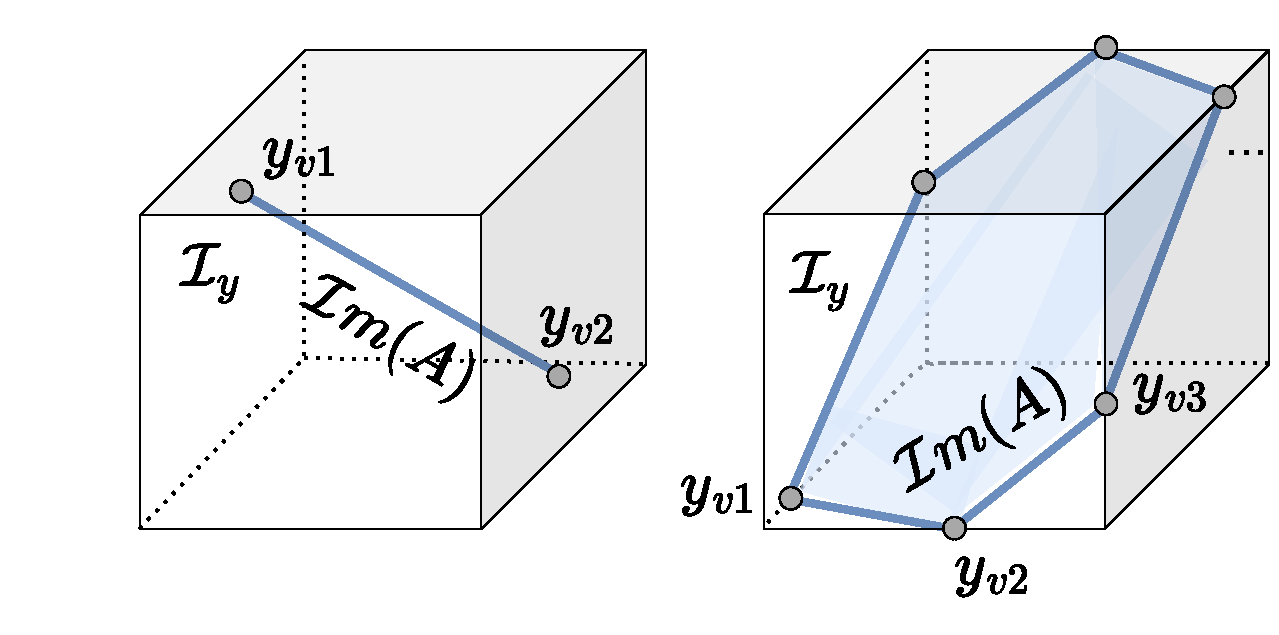
\includegraphics[width=\linewidth]{Papers/images/intersetcion_size.pdf}
    \caption{Example of intersection vertices $\bm{y}_{vi}$ placement on $n\!-\!m$ dimensional faces of hyperrectangle $\mathcal{I}_y$. Left, $m=1$, the vertices $\bm{y}_{vi}$ are on $n\!-\!m\!=\!2$ dimensional faces (sides), while on the right $m=2$ the vertices re on $n\!-\!m\!=\!1$ dimensional faces (edges) }
    \label{fig:size_inter}
\end{wrapfigure}
Sasaki et al. \cite{sasaki_vertex_nodate} have shown that, when the input space dimension is $n$ and the image $\img{A}$ dimension is $m$, the extreme values (vertices) of the intersection $\bm{y}_{v}$ belong to the $n$-$m$ dimensional faces of the hyperrectangle $\mathcal{I}_y$. Figure \ref{fig:size_inter} demonstrates this relationship on an example of with input space dimension $n=3$ and two different output space dimensions $m=1$ and $m=2$. For $m=1$ the vertices $\bm{y}_{v}$ are on $m-n=2$ dimensional faces of the hyperrectangle corresponding to its sides, and when $m=2$ the vertices  $\bm{y}_{v}$ are on $m-n=1$ dimensional faces of the hyperrectangle, its edges.



In order to find the  $\repr{V}$-representation of the intersection  $\mathcal{I}\cap \img{A}$, the state-of-the-art algorithms such as \cite{chiacchio_evaluation_1996} and \cite{sasaki_vertex_nodate} propose an exhaustive search over all the $n$-$m$ dimensional hyperrectangle faces to find the extreme values of $\bm{y}_{vi}$. In this work a new representation of output vector $\bm{y}$ is proposed enabling an efficient navigation of the $n-m$ dimensional hyperrectangle face. Additionally, an efficient approach to discarding the hyperrectangle faces that cannot contain vertices is integrated in the algorithm, further reducing the complexity of the exhaustive search.

\begin{wrapfigure}{r}{0.5\linewidth}
\vspace{-1.6cm}
    \centering
    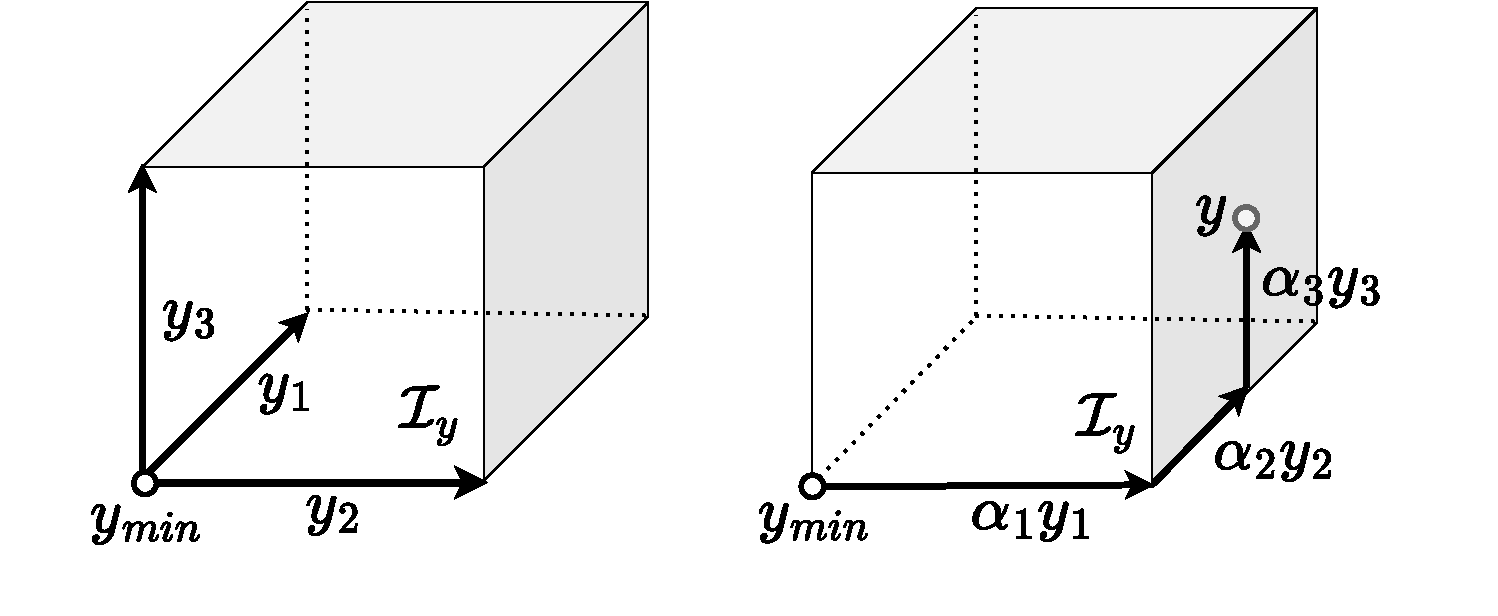
\includegraphics[width=\linewidth]{Papers/images/navigation_y.pdf}
    \caption{Example of the vector representation (\ref{eq:torque_new}) on the $n\!=\!3$ dimensional hyperrectangle $\mathcal{I}_y$. Base vectors $\bm{y}_i$ are shown on the left, and on the right their linear combination using scalars $\alpha_i$ is shown reaching the point $\bm{y}\in\mathcal{I}_y$.}
    \label{fig:navigation_y}
\end{wrapfigure}
\subsection{Proposed algorithm}
Consider an input vector $\bm{y}$ bounded within the input set $\mathcal{I}_y$. It can be defined as
\begin{equation}
    \bm{y} = {\bm{y}}_{min} + \alpha_1 \bm{y}_1+ \alpha_2 \bm{y}_2 + ... + \alpha_n \bm{y}_n
    \label{eq:torque_new}
\end{equation}
where $\alpha_i \in [0,1]$ are scalars weights and vectors $\bm{y}_i$ are orthogonal base vectors in joint space aligned with $i$-th axis of the hyperrectangle $\mathcal{I}_y$, defined as $\bm{y}_i = \begin{bmatrix} 0~\ldots~y_{i,max} - y_{i,min}~\ldots~0 \end{bmatrix}^T$. As shown on the example on Figure \ref{fig:navigation_y}, the input vector $\bm{y}$ representation (\ref{eq:torque_new}) can be exploited to reach any point within the hyperrectangle $\mathcal{I}_y$, by choosing appropriate scalars $\alpha_i$ in range $[0,1]$. Finding the appropriate values of the scalars $\alpha_i$, for any given $\bm{y}$, can be formulated in a form of linear system
\begin{equation}
\underbrace{\begin{bmatrix}
    \bm{y}_1&\cdots&\bm{y}_n
\end{bmatrix}}_{Y_{n\times n}}\underbrace{\begin{bmatrix}
    \alpha_1\\
    \cdots\\
    \alpha_n
\end{bmatrix}}_{\bm{\alpha}_{n\times 1}} = \bm{y}_{min} - \bm{y}, \qquad  \bm{\alpha} = Y^{-1}(\bm{y}_{min} - \bm{y})
\label{eq:define_Y_Alpha}
\end{equation}
where the matrix $Y$, containing the orthogonal base vectors $\bm{y}_i$, is square and always invertible. 
Furthermore, as the intersection vertices $\bm{y}_{vi}$ belong to the $n$-$m$ dimensional faces of the input hyperrectangle $\mathcal{I}_y$, the representation (\ref{eq:torque_new}) can be further simplified. Any input vector $\bm{y}$, belonging to an $n-m$ dimensional face of the hyperrectangle $\mathcal{I}_y$, can be reached by choosing the appropriate values of $n-m$ scalars $\alpha_i\in[0,1]$, while the other $m$ scalars are fixed to either 0 or 1 ($\alpha_i\in\{0,1\}$).

Furthermore, $n-m$ scalars $\alpha_i\in[0,1]$ can be interpreted as coordinates of the $n-m$ dimensional face, while the remaining $m$ fixed scalars $\alpha_i\in\{0,1\}$, to either 0 or 1, define its origin $\bm{y}_o$
\begin{equation}
    \bm{y}_o = \bm{y}_{min} + \alpha_1 \bm{y}_1+ ... + \alpha_m \bm{y}_m, \qquad \alpha_i \in\{0,1\}
\end{equation} 
Then any $\bm{y}$, belonging to a face of the hyperrectangle, can be expressed using the face's origin $\bm{y}_o$ and its set of $n-m$ scalars $\alpha_i$ 
\begin{equation}
    \bm{y} = \bm{y}_o ~+ ~\alpha_{m+1}\bm{y}_{m+1} +~\cdots~ +\alpha_{n}\bm{y}_{n}, \qquad \alpha_i \in [0,1]
\end{equation}
The vector $\bm{\alpha}\in\mathbb{R}^n$ can be conveniently divided into two components, $\bm{\alpha}_o\in\mathbb{R}^m$ containing $m$ scalars $\alpha_i$ defining the origin of the face and $\bm{\alpha}_x\in\mathbb{R}^{n-m}$ containing $n-m$ scalar coordinates $\alpha_i$ of the face. Additionally, the same can be done with the matrix $Y$, divided in $Y_o\in\mathbb{R}^{n\times m}$ corresponding with $m$ base vectors used to define the origins $\bm{y}_o$, and $Y_x\in\mathbb{R}^{n\times (n-m)}$
 corresponding to the $n\!-\!m$ base vectors $\bm{y}_i$ spanning the face. Then the origin $\bm{y}_o$ and the final vector $\bm{y}$ can be expressed as
 \begin{equation}
    \bm{y}_o = \bm{y}_{min} + Y_o\bm{\alpha}_{o}, \qquad \bm{y} = \bm{y}_o +  Y_x\bm{\alpha}_{x}, \qquad \bm{\alpha}_{o}\in\{\bm{0},\bm{1}\},~~ \bm{\alpha}_{x}\in[\bm{0},\bm{1}]
    \label{eq:matrix_new_y}
\end{equation}

Therefore, in order to find all the vertices $\bm{y}_{v}$ of the intersection $\mathcal{I}_y\cap\img{A}$, the proposed algorithm tests if there exists a point intersection (a vertex) between the $\img{A}$ and every single one of the $n-m$ dimensional faces of the hyperrectangle $\mathcal{I}_y$. Since all the $\bm{y}$ belonging to the image $\img{A}$ can be expressed as $\bm{y}=A\bm{x}$, this relationship can be further exploited to relate the vertices $\bm{y}_{v}$ of the intersection $\img{A}\cap\mathcal{I}_y$ and the vertices $\bm{x}_{v}$ of the final polytope $\mathcal{P}_x$. For each face to be tested, the equations  (\ref{eq:inter_hyp_revisit_algo}) and (\ref{eq:compute_vert}) can be combined
\begin{equation}
    \bm{y}_{v} = A \bm{x}_{v} = \bm{y}_{o} + \alpha_{m+1} \bm{y}_{m+1}+ ~...~ + \alpha_n \bm{y}_n \label{eq:step2}
\end{equation}
where, $\bm{y}_o$ is the origin of the $n\!-\!m$ dimensional face, spanned by the scalar $n\!-\!m$ scalars $\alpha_i\in\bm{\alpha}_x$.
Then, for each face, a linear system derived from equation~(\ref{eq:step2}) can be solved to find the $n\!-\!m$ scalars $\alpha_i\in\bm{\alpha}_{x}$ and the corresponding polytope vertex $\bm{x}_{vi}$
\begin{equation}
    \underbrace{\begin{bmatrix}A&-\bm{y}_{m+1} \, \dots \, -\bm{y}_{n} \end{bmatrix}}_{Z_{n\times n}} \begin{bmatrix}\bm{x}_{v}\\ \alpha_{m+1} \\ \vdots\\\alpha_{n} \end{bmatrix} =\begin{bmatrix}A &Y_{x} \end{bmatrix}\begin{bmatrix}\bm{x}_{v}\\ \bm{\alpha}_{x} \end{bmatrix}  = \bm{y}_o, \qquad \begin{bmatrix}\bm{x}_{v}\\ \bm{\alpha}_{x} \end{bmatrix} = Z^{-1}\bm{y}_o, 
    \label{eq:linear_system_full}
\end{equation}
Matrix $Z\in\mathbb{R}^{n\times n}$ is a square matrix where each one of the vectors $\bm{y}_i$ is independent. If the matrix $Z$ is singular, geometrically, the image $\img{A}$ is parallel to the face being tested, therefore no intersections exist. If $Z$ is invertible and the $n-m$ scalars $\alpha_i\in\bm{\alpha}_x$ are obtained, a simple check if $\bm{\alpha}_x \in [\bm{0},\bm{1}]$ can be used to determine if $\bm{x}_{v}$ is a vertex of the polytope $\mathcal{P}_x$. Geometrically, the condition $\bm{\alpha}_x \in [\bm{0},\bm{1}]$ ensures that the intersection point between the $\img{A}$ and the $n\!-\!m$ dimensional face, is also inside $\mathcal{I}_y$.

\begin{wrapfigure}{r}{0.25\linewidth}
\vspace{-1.5cm}
    \centering
    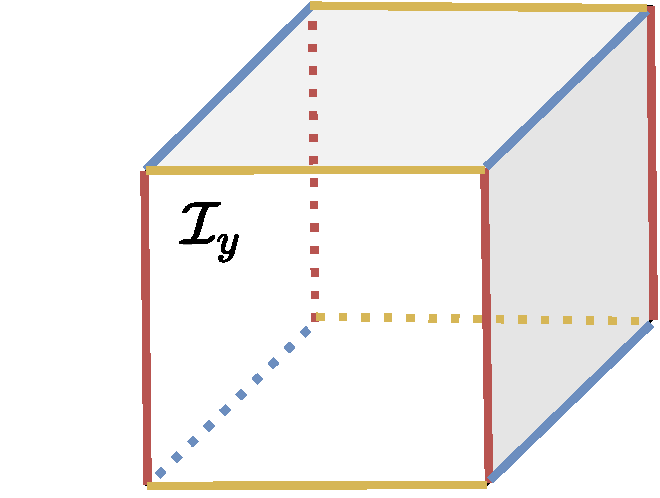
\includegraphics[width=\linewidth]{Papers/images/parallel.pdf}
    \caption{All the parallel edges of the 3D hyperrectangle shown in differing colours. It has 3 (red, blue, yellow) sets of 4 parallel edges, 12 edges in total.}
    \label{fig:parallel}
\end{wrapfigure}

\begin{figure}[!t]
    \centering
    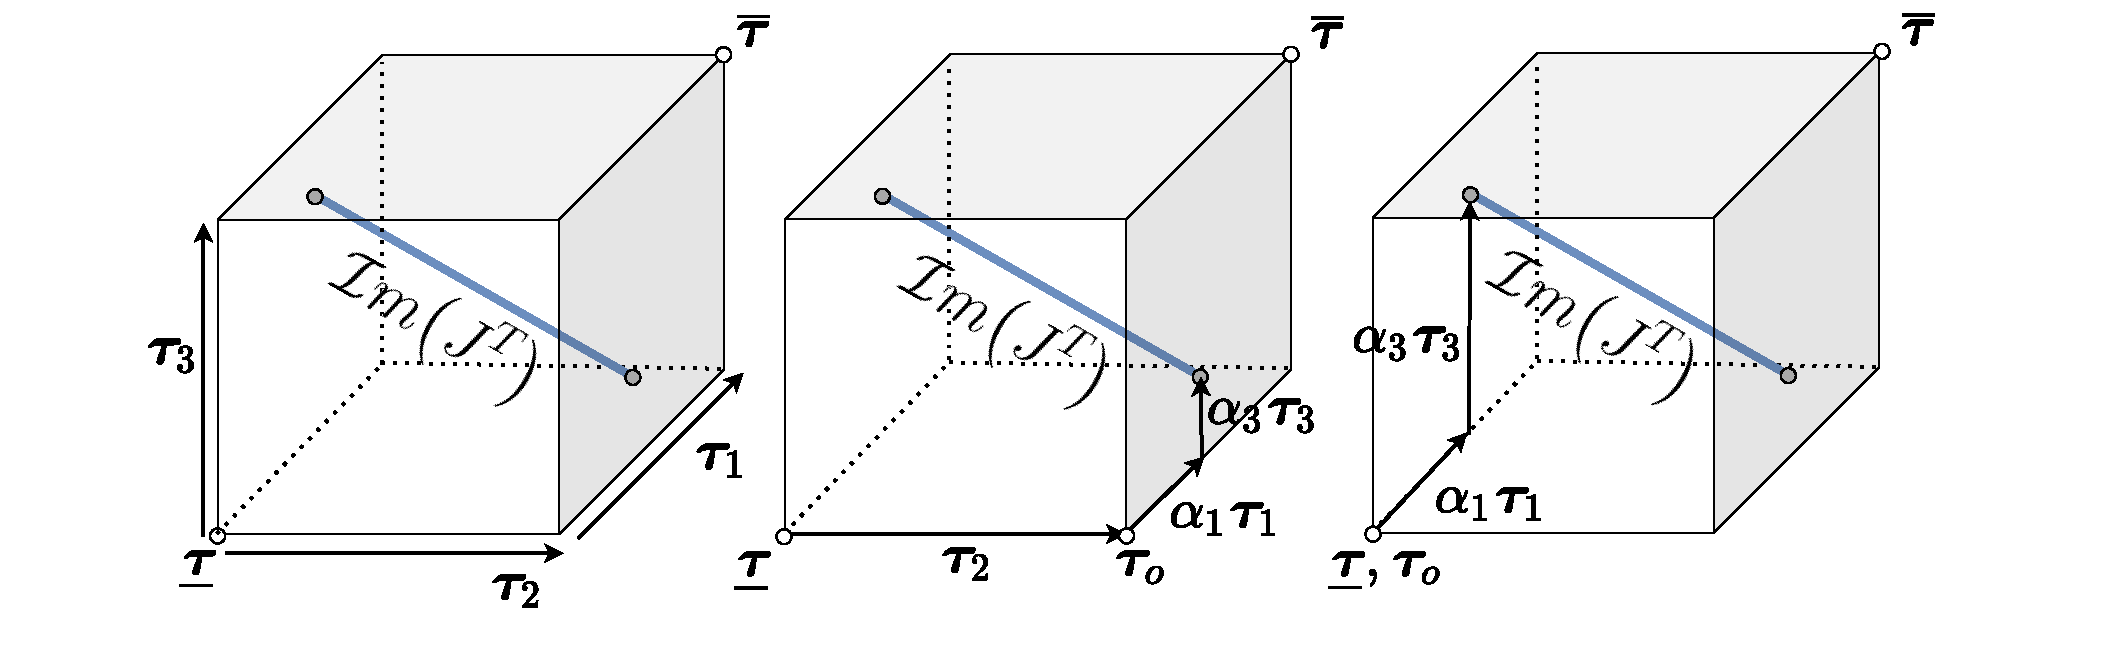
\includegraphics[width=0.9\linewidth]{Papers/images/intersection_example.pdf}
    \caption{Example of input space interpretation of the proposed vertex search algorithm for the system $n$=$3$ and $m$=$1$. The two vertices of the intersection $\{\bm{y}_{v1},\bm{y}_{v2}\}$ are reached by solving the linear system (\ref{eq:linear_system_full}) or (\ref{eq:linear_system_svd}). The vertices belong to the parallel ($n\!-\!m\!=\!2$ dimensional faces) sides of the hyperrectangle $\mathcal{I}_y$.  }
    \label{fig:intersection_example}
\end{figure}

\subsubsection{Exploiting the parallelism} An $n$-dimensional hyperrectangle has $\big(\begin{smallmatrix}n\\m\end{smallmatrix}\big)$ sets of $2^m$ parallel $n\!-\!m$ dimensional faces. As illustrated on Figure \ref{fig:parallel}. a 3D ($n\!=\!3$) hyperrectangle has $\big(\begin{smallmatrix}3\\1\end{smallmatrix}\big)\!=\!3$ sets of $2^{2}\!=\!4$ parallel ($n\!-\!m\!=\!1$) edges, as well as $\big(\begin{smallmatrix}3\\2\end{smallmatrix}\big)=3$ sets of $2^1\!=\!2$ parallel ($n\!-\!m\!=\!2$) sides. 
All the parallel $n\!-\!m$ dimensional faces of the hyperrectangle $\mathcal{I}_y$ have the same set of $n\!-\!m$ scalars $\alpha_i$ as their coordinates, while their origins $\bm{y}_o$ are defined by the remaining $m$ scalars. As there are $m$ scalars $\alpha_i\in\{0,1\}$ characterising every origin $\bm{y}_o$, there are $2^m$ possible origin vectors $\bm{y}_o$ for each set of parallel $n\!-\!m$ dimensional faces. 

Figure \ref{fig:intersection_example} illustrates the case where $\img{A}$ is a line ($m=1$) and the input space is $n=3$ dimensional. In this case the intersection vertices $\{\bm{y}_{v1},\bm{y}_{v2}\}$ lie in $n$-$m$=$2$ dimensional hyperrectangle faces. In that example, both vertices $\bm{y}_{vi}$ are placed on two parallel faces, spanned by the two scalars $\alpha_1$ and $\alpha_3$, while the scalar $\alpha_2$, set to $0$ or $1$, is used to find their origins $\bm{y}_o$.

In the linear system  (\ref{eq:linear_system_full}), the matrix $Z$ has the same content for each parallel face of the hyperrectangle, the inverse $Z^{-1}$ can be recalculated only once per  set of parallel faces. Furthermore, each of the $2^m$ faces in the set will have different origin $\bm{y}_o$, which can then be multiplied with the common $Z^{-1}$ to obtain the vertex $\bm{x}_{v}$ and the corresponding $\bm{\alpha}_x$. 


Overall, in order to navigate all possible combinations of the $n\!-\!m$ dimensional faces which may contain vertices of the intersection $\bm{y}_v$ (and in term the final polytope $\mathcal{P}_x$), the total of $\big(\begin{smallmatrix}n\\m\end{smallmatrix}\big)$=$\frac{n!}{m!(n-m)!}$ inversions of the matrix $Z$ and  $2^m \frac{n!}{m!(n-m)!}$ checks that $\bm{\alpha}_x \in [\bm{0},\bm{1}]$ has to be performed.

In the case depicted in figure \ref{fig:intersection_example} ($n$=$3$, $m$=$1$), $Z$ is inverted only $\big(\begin{smallmatrix}3\\1\end{smallmatrix}\big)$=$3$ times and conditions are evaluated 6 times, which corresponds exactly to the number of sides of the hyperrectangle. In the same example, if the output space would be 2D ($n$=$3$, $m$=$2$) the number of $Z$ inversions is 3 and the number of condition evaluation is 12, which corresponds to the number of edges of the hyperrectangle. One of the nice features of this approach is that it does not require an explicit inversion of $A$, as in equation~(\ref{eq:compute_vert}), to obtain the set of vertices composing $\mathcal{P}_x$.

In the following two sections, two approaches are developed to further improve the efficiency of the porpoised algorithm. First the dimension of the matrix $Z$ is reduced using the Singular Value Decomposition (SVD), then an additional condition is introduced enabling to discard faces and avoid the unnecessary matrix inversions.

\subsubsection{Matrix size reduction using the SVD}

In order to reduce the dimension of the linear system, the Singular Value Decomposition (SVD) \cite{klema_singular_1980} of $A^T$ is used
\begin{equation}
     A^T =  U  \underbrace{\begin{bmatrix}S & O_{m\times (n-m)}\end{bmatrix}}_{\Sigma}\underbrace{\begin{bmatrix}V_1^T \\ V_2^T \end{bmatrix}}_{V^T}
\end{equation}
where $S= diag( \sigma_1 \dots \sigma_m)$ is a diagonal matrix containing the $m$ singular values of $A^T$. $V_1^T \in \mathbb{R}^{m \times n}$ is the projector from the input space onto the image of $\img{A}$ and $V_2^T \in \mathbb{R}^{n-m \times n}$ is a basis of $\ker{A}$. $V_1^T$ and $V_2^T$ are orthogonal vector subspaces yielding $V_2^T V_1 = 0$ and thus 
\begin{equation}
    V_2^T A\bm{x} = \bm{0}
\end{equation}
This allows to reduce (\ref{eq:linear_system_full}) to
\begin{equation}
    \underbrace{V_2^T\begin{bmatrix}-\bm{y}_{m+1} ~\dots~ -\bm{y}_{n} \end{bmatrix}}_{T_{(n-m)\times (n-m)}} \bm{\alpha}_x  = V_2^TY_x\bm{\alpha}_x = V_2^T\bm{y}_o
    \label{eq:linear_system_svd}
\end{equation}
If $T$ is invertible, $\bm{\alpha}_x$ can be computed by
\begin{equation}
\bm{\alpha}_x = T^{-1}V_2^T\bm{y}_o
\end{equation}
When the computed $\bm{\alpha}_x \in [\bm{0},\bm{1}]$,  the corresponding force polytope vertex can be calculated as
\begin{equation}
    \bm{x}_{v} = A^{+} \big( \bm{y}_o + Y_x\bm{\alpha}_x\big)
\end{equation}

This new approach requires the calculation of the SVD and the Jacobian matrix pseudo-inverse $A^{+}$. Nevertheless, since the pseudo-inverse can be efficiently calculated from the SVD as $A^{+} = U\Sigma^{T+}V^T$ and since both the SVD and pseudo-inverse are calculated once per algorithm run, the computation efficiency is greatly improved due to the matrix dimension reduction from $n$ to $(n-m)$ when inverting $T$ instead of $Z$.

\begin{wrapfigure}{r}{0.35\linewidth}
\vspace{-1.4cm}
    \centering
    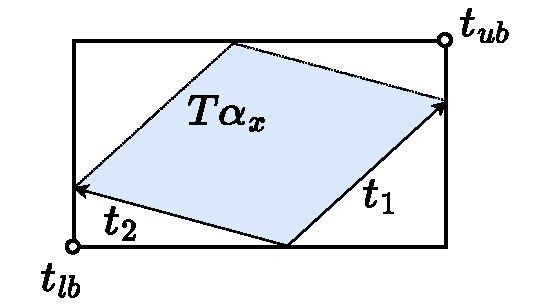
\includegraphics[width=\linewidth]{Papers/images/matrix_condition.pdf}
    \caption{The bounding-box calculated using the equation (\ref{eq:bounds_condition}). The size of the example system is $n\!-\!m\!=\!2$, where $\bm{t}_1,\bm{t}_2$ are column vectors of the matrix $T$.}
    \label{fig:matrix_condition}
\end{wrapfigure}

\subsubsection{Matrix inverse condition}
Due to the constrained nature of $\bm{\alpha}_x$, it is possible to efficiently calculate some bounds ${\bm{t}_{ub}}$ and $\bm{t}_{lb}$ such that $T\bm{\alpha}_x  \in [\bm{t}_{lb}, \bm{t}_{ub}]$, bounding the interval of null-space projections of the vector $\bm{y}_o$.
\begin{equation}
    T\bm{\alpha}_x  = V_2^T\bm{y}_o \in [\bm{t}_{lb}, \bm{t}_{ub}]\label{eq:necesassry_condition}
\end{equation}
As the column vectors $t_i$ within the matrix $T$ are in general case not orthogonal, no min-max interval shaped set can not exactly characterise the feasible set of $T\bm{\alpha}_x$. However, an interval that over-approximates it can be found very efficiently, by row-wise summing only positive and only negative elements $t_{ij}$ of  $T$
\begin{equation}
t_{i,lb} = \sum_j \max(t_{ij}, 0), \qquad
t_{i,lb} = \sum_j \min(t_{ij}, 0) 
\label{eq:bounds_condition}
\end{equation}

As shown on Figure \ref{fig:matrix_condition}, this creates a bounding box around the space defined with the vector $T\bm{\alpha}_x$. Therefore, one can conclude that if all the $2^m$ combinations of $V_2^T\bm{y}_o \notin [\bm{t}_{lb}, \bm{t}_{ub}] $, the system (\ref{eq:linear_system_svd}) cannot have a solution which satisfies $\bm{\alpha}_x \in [\bm{0},\bm{1}]$, and there is no need to invert $T$ to figure it out.

The condition $V_2^T\bm{y}_o \in [\bm{t}_{lb}, \bm{t}_{ub}] $ is a necessary condition, however as the interval $[\bm{t}_{lb}, \bm{t}_{ub}]$ presents an over-approximation of the achievable set $T\bm{\alpha}_x, \bm{\alpha}_x\in[\bm{0}, \bm{1}]$, it is not the sufficient condition.

Including the check for the necessary condition (\ref{eq:necesassry_condition}), results in the reduced number of matrix inversions. The exact number of the matrix inversions per algorithm execution is deterministic for any matrix $A$ and the input set $\mathcal{I}_y$, however unknown in advance. Therefore, the upper bound on the number of matrix inversions $N_i$ can be found by studying the the worst-case scenario, where all the origins $\bm{y}_o$ pass the condition (\ref{eq:necesassry_condition}) in which case the number of inversion corresponds to the binomial $\binom{n}{m}$. In the general case then, the number of matrix inversions $N_i$ is bounded and equals to  
$$N_i\leq\binom{n}{m}=\frac{n!}{m!(n-m)!}$$
The number $N_c$ of checks of the condition $\bm{\alpha}_x \in [\bm{0},\bm{1}]$, per matrix inversion, is bounded as well, as the origin vectors $\bm{y}_o$ that do not comply with the necessary condition (\ref{eq:necesassry_condition}) can be discarded from the these checks as well
$$
N_c\leq2^m
$$

\subsection{Performance and complexity comparison}\label{sec:complexity}
To demonstrate the efficiency of the proposed polytope vertex search algorithm, it is compared to the polytope vertex search algorithm introduced by Chiacchio et al. \cite{chiacchio_evaluation_1996}. Furthermore the comparison is extended to the algorithm proposed by Sasaki et al. \cite{sasaki_vertex_nodate} which is, to our knowledge, the only algorithm exploiting the geometric structure of the intersection formulation polytope with interval limits (\ref{eq:inter_hyp_revisit_algo}).


\begin{table}[!h]
    \centering
    \caption{Complexity and execution time (in milliseconds) comparison for three different vertex search algorithms. The comparison provided for the number of matrix inversions, matrix size and time of execution, averaged over 1000 random systems. }
    \begin{tabular}{|c|c|c|c|}
       \hline
      \textbf{ System size }& \textbf{Chiacchio}\cite{chiacchio_evaluation_1996} & \textbf{Sasaki} \cite{sasaki_vertex_nodate}  &  \textbf{Proposed} \\
       \hline
       $(n,m)$& matrix inversions: $ \frac{2n!}{m!(2n-m)!}$  & $ \frac{n!}{m!(n-m)!} $ & $ \leq \frac{n!}{m!(n-m)!}$ \\
       &  matrix size:  $ 2n \times 2n$ & $m\times m$  & $n$-$m$ $\times$ $n$-$m$\\
       & time[ms]: mean $\pm$ std (max) & & \\
       \hline
       $(4,2)$ &  24 & 6 & 4.2$\pm$1.4 (6) \\ 
       & 8$\times$8 & 2$\times$2 & 2$\times$2 \\ 
       & 2.7$\pm$0.1 (3.6) & 0.93$\pm$0.1 (1.1) & 0.64$\pm$0.1 (1.5) \\ 
       \hline
       $(4,3)$ &  32 & 4 & 2.9$\pm$1.1 (4) \\ 
       & 8$\times$8 & 3$\times$3 & 1$\times$1 \\ 
       & 3.7$\pm$0.3 (6.0) & 0.79$\pm$0.08 (1.4) & 0.54$\pm$0.1 (1.4) \\ 
       \hline
       $(6,3)$ & 220 & 20 & 2.8$\pm$2.5 (10) \\ 
        & 12$\times$12 & 3$\times$3 & 3$\times$3 \\ 
       & 14.2$\pm$0.9 (20) & 2.1$\pm$0.2 (3.4) & 1.5$\pm$0.2 (2.7) \\ 
       \hline
      $(6,6)$&   64 & 1 & 1$\pm$0 (1)\\
        &  12$\times$12 & 6$\times$6 & 6$\times6$\\
       & 34.7$\pm$1 (44.3) & 0.32$\pm$0.07 (0.56) & 0.24$\pm$0.04 (0.46)\\
       \hline
      $(7,3)$&    364 & 35 & 7.3$\pm$4.2 (20)\\
        & 14$\times$14 & 3$\times$3 & 4$\times4$\\
       & 25$\pm$0.5 (27) & 3.5$\pm$0.1 (5.4) & 2.6$\pm$0.2 (4.3)\\
       \hline
      $(7,6)$& 448 & 7 & 6.4$\pm$1 (7)\\
        & 14$\times$14 & 6$\times$6 & 1$\times$1\\
       & 150$\pm$34 (360) & 1.6$\pm$0.5 (4) & 1.2$\pm$0.3 (3.0)\\
       \hline
    \end{tabular}
    \label{tab:complexity_results}
\end{table}

\todos{Talk about the $m=6$}

The three algorithms have been tested on finding the $\repr{V}$-representation of the three different systems, inspired by the force ($\bm{f}\in\mathbb{R}^3$, $m=3$) polytope $\mathcal{P}_f$ enumeration for three different robots: a 4R planar robot ($n$=$4$, $m$=$2$), the \textit{Universal Robots} UR5 6DoF robot ($n$=$6$, $m$=$3$) and the \textit{Franka Emika Panda} 7DoF robot ($n$=$7$,$m$=$3$). The results are averaged over 1000 randomly generated matrices $A$ and input sets $\mathcal{I}_y$. All algorithms have been implemented in the programming language Python and tested on a laptop equipped with a 1.90GHz Intel i7-8650U processor. 

Table \ref{tab:complexity_results} shows the results of this complexity evaluation. The proposed vertex search algorithm substantially reduces the number of matrix inversions and thus reduces the processing time considerably: $4$-$10\times$ faster execution than Chiacchio's algorithm and on average 30\% faster than Sasaki's. Results show that even for the generic cases that correspond to the 6DoF ($n=6$,$m=3$) and 7DoF ($n=7$,$m=3$) industrial robots the proposed approach is capable of evaluating the polytope vertices under $3ms$. Such a low processing time opens numerous opportunities for the on-line use of polytope based capacity evaluation especially in the area of robot control.

\begin{figure}
    \centering
    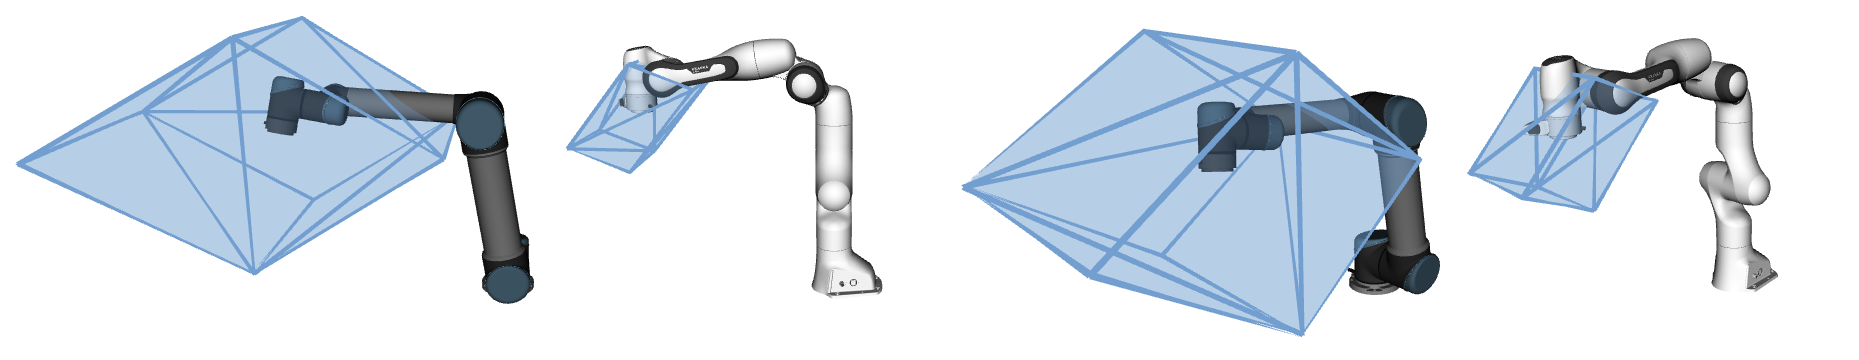
\includegraphics[width=\linewidth]{Papers/images/panda_ur5.png}
    \caption{Two different views of Panda ($n=7$) and UR5 ($n=6$) robot's force polytope ($m=3$) calculated using the proposed algorithm. Both robots and polytopes are shown in the same scale (1m : 1000N). The figure shows that the UR5 has much larger polytope than Panda robot. This is due to its larger force capacity, as UR5 is rated for 5kg loads whereas Panda is rated for 3kg loads.}
    \label{fig:panda_ur5_force}
\end{figure}
\todos{Talk about the Figure \ref{fig:panda_ur5_force}}

\subsection{Discussion on limitations}
This algorithm, being based on the algorithm proposed by Sasaki \cite{sasaki2011vertex}, is still based on the exhaustive search. Even though significantly reducing the complexity of the Sasaki's method, it is not particularly well suited for high dimensions $n$ of the input spaces, especially is the difference between the input and the output space dimension $n\!-\!m$ is large. 

The algorithm has two computational bottlenecks: the number of matrix $T$ inversions $N_i$ and the number of checks $\bm{\alpha}_x \in [\bm{0},\bm{1}]$ per matrix inversion $N_c$.

If the system has high dimensional input space and low dimensional output space ($n\gg m$) then the number of matrix inversions $N_i=\binom{n}{m}$ will be large, while the number of checks $N_c=2^m$  will be low. 
On the other hand, if the system has both high dimensional input space and the high dimensional output space ($n\approx m$ and $n,m\gg0$), then the number of matrix inversions $N_i=\binom{n}{m}$ will be relatively low and will not be the limiting factor, but the number of checks $N_c=2^m$ which will be very high. Therefore, although the algorithm is created in a generic form and can find the $\repr{V}$-representation of any polytope belonging to this family, it is particularly efficient when the dimensions of the input and the output space are relatively low. 

Furthermore, as the proposed algorithm exploits the null-space $\ker{A}$ of the matrix $A$ to gain on efficiency, it is not suitable for the systems where the matrix $A$ is square ($m\!=\!n$), as in that case the null-space does not exist $\ker{A}=\{\varnothing\}$. However, as discussed in the section \ref{par:equivalent_proj}, this specific case of interval projection is much easier to work with as it corresponds to the projection formulation, which $\repr{V}$-representation can be determined in a straight-forward manner, as described in section \ref{ch:proj_algos_v}, by projecting the vertices of the hyperrectangle to the output space.


\begin{algorithm}[!b]
\caption{The proposed vertex search algorithm pseudo-code}
\begin{algorithmic}
\REQUIRE $A$, $\bm{y}_{min}$, $\bm{y}_{max}$ (Eq. \ref{eq:interval_revisit_algo}) 
\STATE $U, \Sigma, V^T \leftarrow svd(A^T)$ 
\STATE $A^{+} = U\Sigma^{T+}V^T$
\STATE $V_1,\, V_2  \leftarrow V $
\STATE calculate $n$ base vectors $\bm{y}_1 \dotsc \bm{y}_n$ (Eq. \ref{eq:torque_new})

\STATE init $\repr{V}$-rep: $X_v$, $Y_v$ $\!\leftarrow\! []$

\FORALL{  $\big(\begin{smallmatrix}n\\m\end{smallmatrix}\big)$ combinations of $m$ fixed $\alpha_i$ } 
\STATE construct matrices $Y_o$ and $Y_x$
\STATE $T = V_2^TY_x$
\IF{matrix T invertible}
\STATE find bounds $\bm{t}_{lb},\bm{t}_{ub}$ (Eq. \ref{eq:bounds_condition})
\STATE init list of origins $\bm{y}_o$ satisfying the condition (Eq. \ref{eq:necesassry_condition}): $L_o$ $\!\leftarrow\! []$ 
\FORALL{   $2^m$ vectors $\bm{\alpha}_o$ }
\STATE $\bm{y}_o = \bm{y}_{min} +  Y_o\bm{\alpha}_o$ 
\IF{$ V_2^T\bm{y}_o \in [\bm{t}_{lb},\bm{t}_{ub}] $}
\STATE update candidates: $L_o \!\leftarrow\! [L_o,~ \bm{y}_o]$
\ENDIF
\ENDFOR

\IF{$L_o$ not empty}
\STATE calculate the inverse $T^{-1}$
\FORALL{   $\bm{y}_o$ in $L_o$ }
\STATE $\bm{\alpha}_x = T^{-1}V_2^T\bm{y}_o $
\IF{$ \bm{\alpha}_x \in [\bm{0},\bm{1}] $}
\STATE $\bm{y}_{v} = \bm{y}_o + Y_x\bm{\alpha}_x$ 
\STATE $\bm{x}_{v} = A^{+}\bm{y}_{v}$ 
\STATE update $\repr{V}$-rep: ${X}_{v} \!\leftarrow\! [{X}_{v},~ \bm{x}_v ]$, ${Y}_{v} \!\leftarrow\! [{Y}_{v},~ \bm{y}_v ]$ 
\ENDIF
\ENDFOR
\ENDIF


\ENDIF

\ENDFOR
\RETURN $\repr{V}$-rep: $X_v$, $Y_v$

\end{algorithmic}
\label{alg:algo_1}
\end{algorithm}

\subsection{Algorithm summary}
This section introduces a new vertex search algorithm for efficient finding of $\repr{V}$-representation of polytopes with the intersection formulation (\ref{eq:inter_poly}) and the interval input set $\mathcal{I}_y$. The algorithm exploits the geometry of the hyperrectangle structure of the interval input set $\mathcal{I}_y$ in order reduce the complexity of the vertex search. The algorithm is based on the algorithm proposed by Sasaki et al.~\cite{sasaki2011vertex} which is based on the extensive search in the $n$ dimensional input space. The proposed algorithm, by further leveraging the geometry of the problem, reduces the search space for the extensive search and significantly reduces both the computational complexity and the execution time of the original method.

The algorithm is particularly well suited for the polytope formulations with relatively low input and output dimensions, that are very common when characterising the physical abilities of robotic manipulators. For example for enumerating the vertices of the wrench capacity polytope of the robotic systems, as described in section \ref{ch:poly_force}. As shown in the comparative analysis with the state-of-the-art methods, in section \ref{sec:complexity},  in the case of enumerating the wrench capacity polytopes of standard robotic manipulators, the algorithm has the execution time of a couple of milliseconds (implemented in python), opening doors for their use in online applications.

The pseudo-code of the proposed algorithm is given in Algorithm \ref{alg:algo_1}, while an efficient open-source python implementation is publicly available within the package \textsc{pycapacity}\footnote{https://auctus-team.github.io/pycapacity/}, which is described more in detail in chapter \ref{ch:software}.

Finally, section \ref{ch:robot_robot_carrying} brings the application of the proposed algorithm for the real-time robot control in the human-robot collaboration scenario, where the algorithm is exploited in order to calculate the robot's wrench capacity polytope online. 

% In this section, a new algorithm for polytope approximation is introduced, developed for the generic polytope formulation
% \begin{equation}
%     \mathcal{P}_x = \big\{ \bm{x}\in \mathbb{R}^{m}\, |\,A\bm{x} = B\bm{y} + \bm{b}, \quad  \bm{y}\in\mathcal{P}_y  \big\}
%     \label{eq:generic_polyt_view_revisit2}
% \end{equation}
% where the input set $\mathcal{P}_y$ can be expressed with its $\repr{H}$-representation
% \begin{equation}
%     \mathcal{P}_y = \big\{ \bm{y}\in \mathbb{R}^{n}\, |\,H_y\bm{y} \leq \bm{d_y}\big\}
%     \label{eq:generic_poly_input_set_revisit2}
% \end{equation} 
% The algorithm is based on the Convex-Hull Methods (CHM) \cite{lassez1992quantifier}, described in section \ref{ch:approximation_algos}. The CHM algorithms are approximation methods that refine the final polytope approximation iteratively until the approximation error is reduced within user defined level. 
% As discussed in section \ref{ch:collab_metrics_overview}, the generic polytope formulation (\ref{eq:generic_polyt_view_revisit2}) unifies the formulations of all the common polytope characterisations of human's and robot's physical abilities, making the algorithm applicable to the transformation of all of their polytope formulations described in section \ref{ch:poly_metrics}. The correspondence of different physical ability polytopes and the generic formulation (\ref{eq:generic_polyt_view_revisit2}) is described in table \ref{tab:merged_table}. Even thought the algorithm can be applied to all the polytope formulations corresponding to (\ref{eq:generic_polyt_view_revisit2}) and its special cases, it is particularly well suited for cases where the dimension of the input space is high ($n\gg m$) and the dimension of the output space is relatively low ($m\leq3$). 

% The generic polytope formulation (\ref{eq:generic_polyt_view_revisit2}) has an implicit form $A\bm{x}=B\bm{y}$ which is not suitable for standard polytope transformation strategies described in section \ref{ch:polytope_algorithms}. Its formulaiton corresponds to the intersection-projection formulation, introduced in section \ref{ch:inter_proj_form}, which can be seen as a special case of the intersection formulation 
% \begin{equation}
%     \mathcal{P}_x \in \{\bm{x}\in \mathbb{R}^m~|~A \bm{x} = \bm{z} + \bm{b},~ \bm{z} \in \mathcal{P}_z\} 
% \end{equation}
% where the input set polytope $\mathcal{P}_z\in\mathbb{R}^k$ is defined using the projection formulation
% \begin{equation}
%     \mathcal{P}_z \in \{\bm{z}\in \mathbb{R}^k~|~z = B\bm{y},~ \bm{y} \in \mathcal{P}_y\} 
% \end{equation}

% Finding the $\repr{V}$ and $\repr{H}$-representation of this polytope, using the standard methods, requires separating the problem and first transforming the input set $\mathcal{P}_z$ in a suitable representation, followed by the second step of transforming the final polytope $\mathcal{P}_x$. 

% When the input space is high dimensional $n\gg0$, both polytope $\mathcal{P}_z$ and $\mathcal{P}_x$ have complex geometries, consisting in large number of vertices and faces. In such cases, the exact polytope transformation methods have intractable computation times, relaying on the exhaustive search in the high $n$ dimensional input space. 

% As discussed in section \ref{ch:approximation_algos}, different polytope approximation methods, in such cases, enable an efficient polytope transformation by operating in the low ($n\gg m$) dimensional output space. The approximation methods based on CHM algorithms, provide an efficient incremental approximation of the polytope $\mathcal{P}_x$ while at the same time guaranteeing an user defined bound on the approximation accuracy. Furthermore, these methods find the $\repr{H}$ and $\repr{V}$-representation at the same time. However, the CHM methods in their original form are not suitable to the implicit polytope formulation (\ref{eq:human_force_poly_revisit2}). 

% Therefore this section proposes a CHM based iterative algorithm for polytope approximation adapted to the generic polytope formulation (\ref{eq:human_force_poly_revisit2}).




\section{New algorithm for polytope approximation}
\label{ch:algorihtm_ichm}

This section introduces a new Convex-Hull Method (CHM) based algorithm for polytope approximation tailored specifically for the generic polytope formulation
\begin{equation}
    \mathcal{P}_x = \big\{ \bm{x}\in \mathbb{R}^{m}\, |\,A\bm{x} = B\bm{y} + \bm{b}, \quad  \bm{y}\in\mathcal{P}_y  \big\}
    \label{eq:generic_polyt_view_revisit2}
\end{equation}
where the input set $\mathcal{P}_y$ can be expressed with its $\repr{H}$-representation
\begin{equation}
    \mathcal{P}_y = \big\{ \bm{y}\in \mathbb{R}^{n}\, |\,H_y\bm{y} \leq \bm{d_y}\big\}
    \label{eq:generic_poly_input_set_revisit2}
\end{equation} 
This polytope formulation, as discussed in section \ref{ch:collab_metrics_overview}, unifies the formulations of all the common polytope characterisations of human's and robot's physical abilities. The correspondence of different physical ability polytopes and the formulation (\ref{eq:generic_polyt_view_revisit2}) can be found in table \ref{tab:merged_table}. 

The generic polytope formulation (\ref{eq:generic_polyt_view_revisit2}) has an implicit form $A\bm{x}=B\bm{y}$ which cannot be used directly with standard polytope transformation strategies described in section \ref{ch:polytope_algorithms}. More specifically, its formulation corresponds to the intersection-projection, introduced in section \ref{ch:inter_proj_form}, a special case of the intersection formulation 
\begin{equation}
    \mathcal{P}_x \in \{\bm{x}\in \mathbb{R}^m~|~A \bm{x} = \bm{z} + \bm{b},~ \bm{z} \in \mathcal{P}_z\} 
\end{equation}
where the input set polytope $\mathcal{P}_z\in\mathbb{R}^k$ is defined using the projection formulation
\begin{equation}
    \mathcal{P}_z \in \{\bm{z}\in \mathbb{R}^k~|~z = B\bm{y},~ \bm{y} \in \mathcal{P}_y\} 
\end{equation}
Finding the $\repr{V}$ and $\repr{H}$-representation of the polytope $\mathcal{P}_x$, using the standard methods, requires separating the problem and first transforming the input set $\mathcal{P}_z$ in a suitable representation (usually $\repr{H}$), followed by the second step of transforming the final polytope $\mathcal{P}_x$. 

However, when the input space is high dimensional $n\gg1$, both polytope $\mathcal{P}_z$ and $\mathcal{P}_x$ have complex geometries, consisting in large number of vertices and faces. The high dimensional input space (and low dimensional output spaces $n\gg m$) are very common when it comes to characterising the physical abilities of humans, based on their musculoskeletal modes. The musculoskeletal models often have large number of muscles $n\gg1$, often more than 50, while the output space usually corresponds to the 3D cartesian space ($m=3$). In such cases, the exact polytope transformation methods have intractable computation times, as they relay on the exhaustive search in the high dimensional input space.

To overcome the complexity of the exhaustive search, various approximate approaches, such as the Ray Shooting Method (RSM)  \cite{agarwal1993ray} and the Convex-Hull Method (CHM) \cite{lassez1992quantifier} described in section \ref{ch:approximation_algos}, have been developed, reducing the computation complexity and improving the execution time. 
Although RSM algorithms are relatively simple to setup they do not provide any bound on their estimation error and highly rely on hand tuned initial parameters. 
CHM \cite{lassez1992quantifier} algorithms on the other hand, perform a very efficient iterative approximation,  while at the same time guaranteeing the bound of the user defined approximation error. In each iteration CHM refines the approximation, by using the Linear Programming (LP) to find new vertices of the polytope and Convex-Hull to group them to faces. Furthermore, CHM finds the $\repr{V}$ and the $\repr{H}$-representation of the polytope at the same time. However in its standard formulation, the CHM is not suitable for the family of problems given with equation (\ref{eq:generic_polyt_view_revisit2}). 

Therefore, this section proposes a new algorithm extending the CHM algorithm to the generic polytope formulation (\ref{eq:generic_polyt_view_revisit2}). Section \ref{ch:lp_adapt} introduces the LP formulation adapting the CHM approach to the implicit problem formulation (\ref{eq:generic_polyt_view_revisit2}), while section \ref{ch:method} brings proposed algorithm overview, as well as the pseudo-code and the geometrical representation. Finally, section \ref{ch:chm_performance} brings the performance analysis of the proposed method and comparison to the state-of-the-art methods on the example of finding the $\repr{V}$-representation of the human wrench capacity polytope based on the musculoskeletal models, which is particularly challenging both due its implicit formulation and high dimensional input space $n\gg m$.

\subsection{Linear programming formulation}
\label{ch:lp_adapt}

\begin{wrapfigure}{r}{0.32\linewidth}
    \centering
    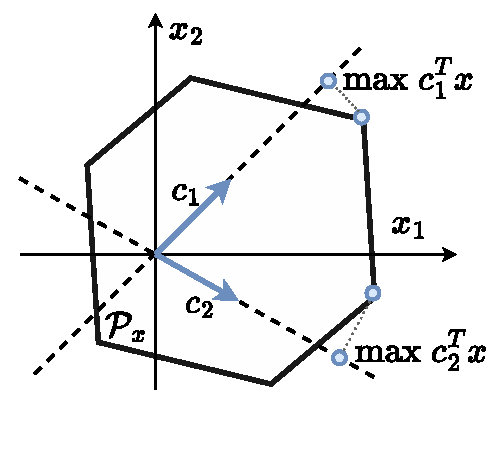
\includegraphics[width=\linewidth]{Papers/images/lp_explication.pdf}
    \caption{The figure demonstrates the LP based vertex search by choosing two different vectors $\bm{c}$.}
    \label{fig:lp_explication}
\end{wrapfigure}
From a geometrical point of view, solving a linear programming (LP) problem boils down to finding a vertex of a polytope \cite{vajda_gass_1964}. 
\begin{equation}
\begin{aligned}
    \bm{x}_v = \text{arg}\max_{\bm{x}} \quad &  \bm{c}^T\bm{x} \\
     \textrm{s.t.} ~~&\bm{x} \in \mathcal{P}_x \\
\end{aligned}
\label{eq:lin_prog}
\end{equation}
However, in order for the polytope $\mathcal{P}_x$ to be suitable for LP optimisation in the $m$-dimensional output space, its implicit formulation $A\bm{x}=B\bm{y}$ needs to be expressed in explicit form.

In the general case, input space is higher dimensional $n\geq m$ and the matrix $A$ is not square. As discussed in section \ref{par:equivalent_proj}, , to find an explicit form of equation (\ref{eq:generic_polyt_view_revisit2}), the pseudo-inverse $A^+$ can be used as a solution only if $B\bm{y}+\bm{b}$ belongs to the image $\img{A}$ of $A$ \cite{klema_singular_1980}. Therefore, equation 
\begin{equation}
    A\bm{x} = B\bm{y} + \bm{b}
\end{equation} 
can be transformed to 
\begin{equation}
    \bm{x} = A^{+} (B \bm{y} + \bm{b}), \qquad \text{where} \quad B\bm{y} + \bm{b} \in \mathcal{I}m(A)
    \label{eq:eq_general_red}
\end{equation} 

Using the Singular Value Decomposition (SVD) \cite{klema_singular_1980} of the matrix $A$ transposes produces $A^T = U\Sigma V^T$. The rotation matrix $V \in \mathbb{R}^{n\times n }$ is separated into  $V_1\in \mathbb{R}^{n\times m}$, a projector to the image $\img{A}$ of $A$, and $V_2\in \mathbb{R}^{n\times(n-m)}$, a projector to its null-space $\ker{A}$. As all the vectors belonging to of the image $\img{A}$ have zero projection to the null-space $\ker{A}$, an equality constraint can be devised for $B\bm{y}+\bm{b}$ to belong to the image $\img{A}$ of $A$. 
\begin{equation}
    V_2^TB\bm{y} +V_2^T\bm{b}  = \bm{0}
    \label{eq:nullspace_gen}
\end{equation}

Finally, combining equations (\ref{eq:nullspace_gen}), (\ref{eq:eq_general_red}), (\ref{eq:generic_poly_input_set_revisit2}) and (\ref{eq:generic_polyt_view_revisit2}), one can create a Linear Program (LP) capable of reaching all vertices of the polytope $\mathcal{P}_x$
\begin{equation}
\begin{aligned}
    \max_{\bm{y}} \quad &  \bm{c}^TA^{+}B\bm{y} + A^{+}\bm{b}\\
     \textrm{s.t.} \quad &  V_2^TB\bm{y} = -V_2^T\bm{b} \\
          & ~~~  H_y \bm{y} \leq \bm{d}_y \\
\end{aligned}
\label{eq:lin_prog}
\end{equation}
by appropriately choosing the projection $\bm{c}$, as demonstrated on Figure \ref{fig:lp_explication}.



\subsection{Proposed algorithm overview}
\label{ch:method}

Given the polytope definition (\ref{eq:generic_polyt_view_revisit2}) and the LP problem defined in (\ref{eq:lin_prog}), the proposed method provides a structured way to choose vectors $\bm{c}$ to find all the vertices ($\repr{V}$-representation) and facets ($\repr{H}$-representation) of the polytope $\mathcal{P}_x$. 
In order to do so, the method leverages the iterative convex hull $\mathcal{C}$ calculation, where each newly found vertex extends $\mathcal{C}$. The normal vectors of the faces of the newly obtained $\mathcal{C}$ are used to decide for the new vectors $\bm{c}$ to use in the LP (\ref{eq:lin_prog}). This iterative process is performed until some specified level of accuracy is reached. Figure \ref{fig:algo_example} visually demonstrates several iterations of the algorithm for the 2-dimensional polytope $\mathcal{P}_x$ example.

\subsubsection{Initial convex hull}More precisely, the first step of the algorithm constructs an initial set of vertices $\bm{x_v}$ and an initial convex hull $\mathcal{C}$. In a $m$-dimensional space, the minimal number of points to create a volume is $m\!+\!1$.  There are various ways proposed in the literature to obtain the initial set of points in order to start the refinement process, such as starting by a random set of directions $\bm{c}$ proposed by Lassez et al. \cite{lassez1992quantifier} in their original paper. Another approach, proposed by Del Prete et al. \cite{DelPrete2016Fast} proposes to uniformly sample the input space.

The approach proposed in this work exploits the base vectors $\bm{u}_i\in U$ obtained using the Singular Value Decomposition of the matrix $(A^+B) = U\Sigma V^T$. This approach has two benefits. One one hand, the base vectors $\bm{u}_i$ are orthogonal vectors in the output space corresponding to the 
highest variability (amplification) directions, given by the singular values $\sigma_i$ of the matrix $A^+B$.
Therefore, the chances of not obtaining $m-1$ different vertices when projecting the polytope $\mathcal{P}_x$ in these directions is much lower than in random directions. And on the other hand, for any matrix $A$ and $B$, the matrix $U$ is relatively efficient to calculate.

Therefore, the porpoised approach to find the initial set of vertices consists in solving two LPs (\ref{eq:lin_prog}) for each one of the $m$ base vectors $\bm{u}_i$, one that minimises ($\bm{c} = -\bm{u}_i$) and one maximises ($\bm{c} = \bm{u}_i$) the projection of the polytope $\mathcal{P}_x$. In the ideal case, this approach obtains $2m$ vertices of the polytope $\mathcal{P}_x$. Once the initial set of vertices $\bm{x}_v$ is found, the initial convex hull $\mathcal{C}$ can be calculated. Its centroid position is given by $\bm{x}_c\!=\!\frac{1}{N}\!\sum\bm{x}_{v,i}$. 



\begin{figure}[!t]
    \centering
    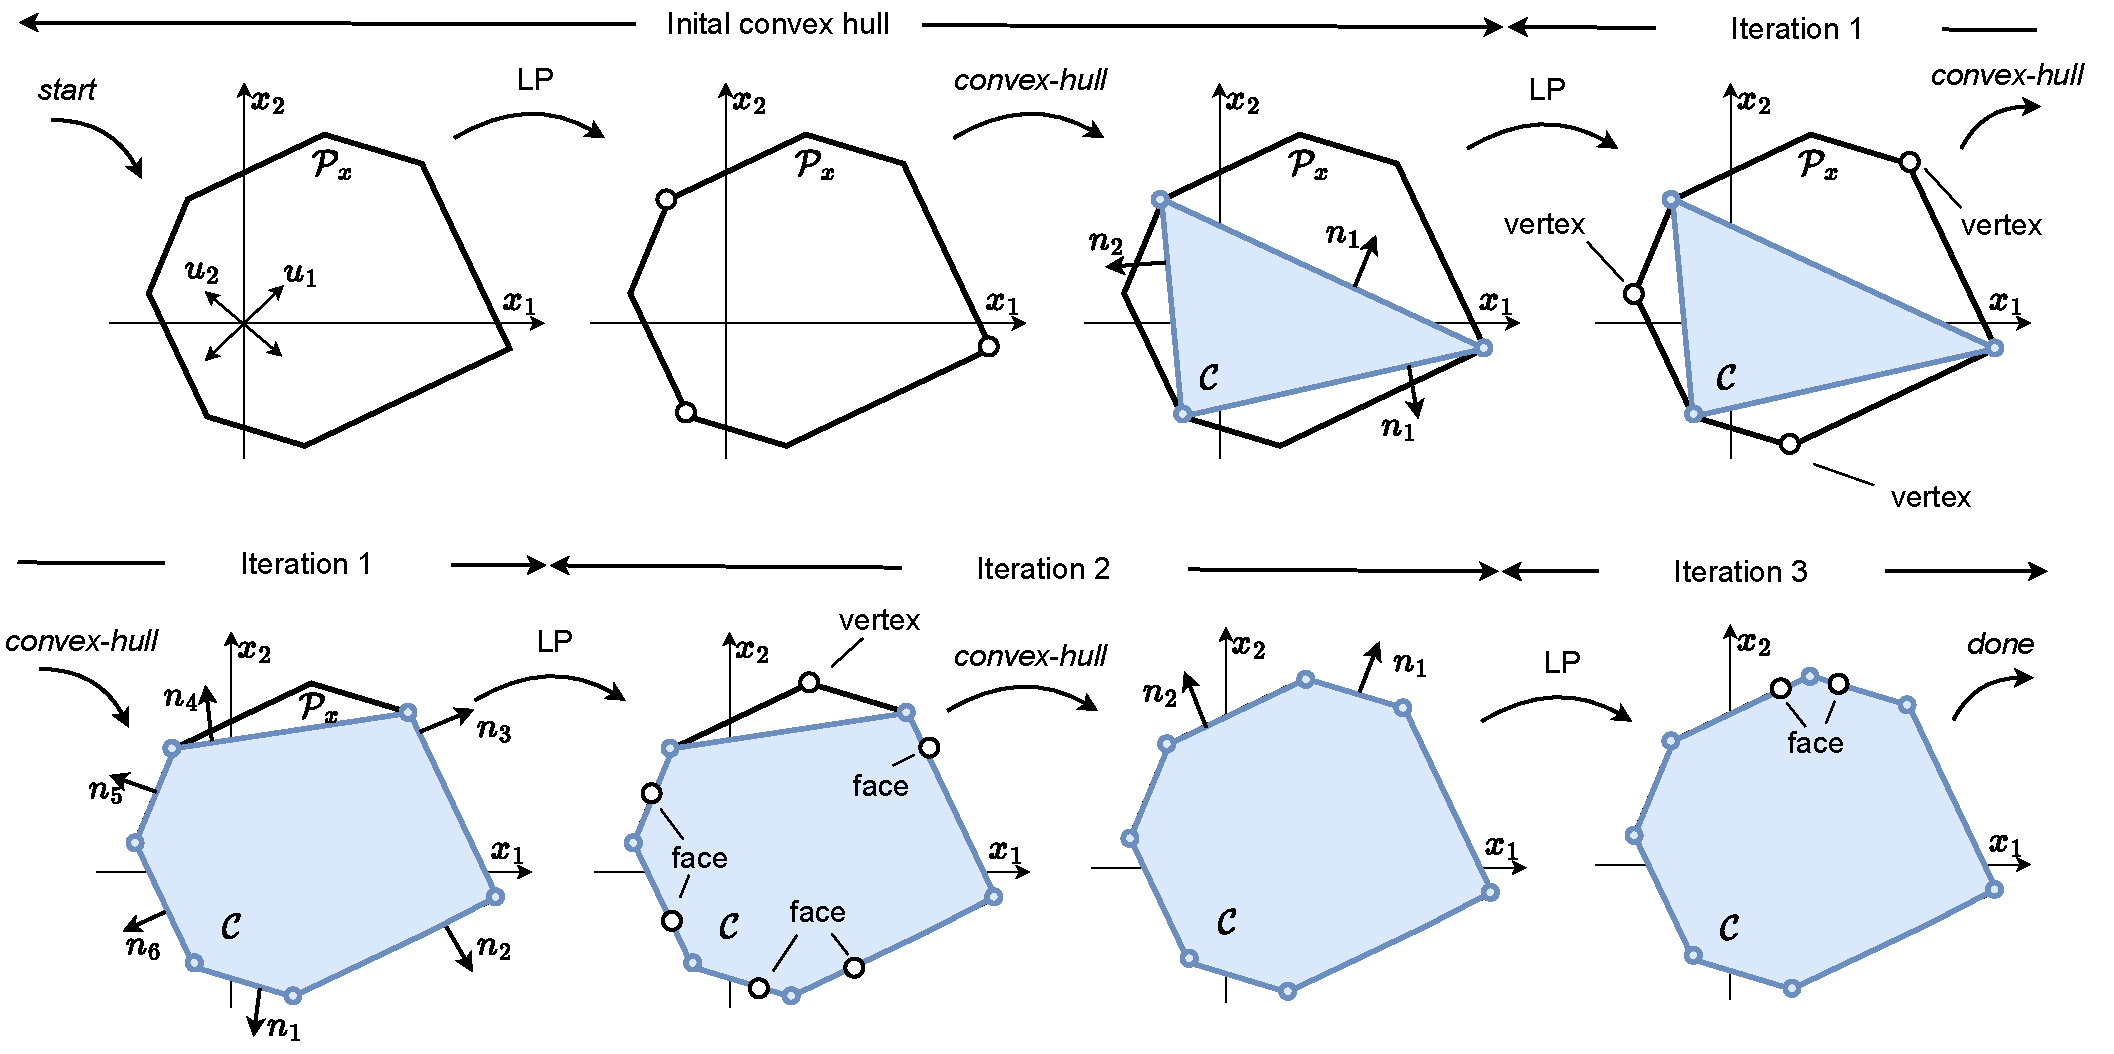
\includegraphics[width=\linewidth]{Papers/images/ichm_full.pdf}
    \vspace{-0.8cm}
    \caption{This figure shows the procedure of the successive approximation of the polytope $\mathcal{P}_x$ using the proposed CHM algorithm. The approximation starts with the initial convex-hull $\mathcal{C}$ construction, using the vectors $\bm{u}_i\in U$. Then the approximation is refined by using the face normal vectors $\bm{n}_i$ of the convex-hull $\mathcal{C}$ with the LP (\ref{eq:lin_prog}) to find new vertices which are then used to update the convex-hull $\mathcal{C}$. The check (\ref{eq:normal_coplanar_test} is used to determine if the LP results belong to the faces or they are new vertices of the polytope. The algorithm stops when no new vertices are found. }
    \label{fig:algo_example}
\end{figure}


\subsubsection{Incremental refinement} The next step of the algorithm is to iterate over all the faces $\mathcal{F}_i$ of the convex hull $\mathcal{C}$. For each new face $\mathcal{F}_i$, the normal $\bm{n}_i$ is found and used as a candidate $\bm{c}_i$ in the direction pointing out of polytope $\mathcal{P}_x$.
%all the vertices $\bm{x}_{\mathcal{F}j}\! =\! %\bm{x}_v\!\in\!\mathcal{F}_i$. Then the $\bm{c}_i$ is defined %as normal $\bm{n}_i$ in the direction pointing out of the polytope 5$\mathcal{P}_x$.
The normal vector direction is verified by projecting the vector going from the centroid $\bm{x}_c$ to any vertex $\bm{x}_{j}$ of face $\mathcal{F}_i$, onto the normal $\bm{n}_i$ and verifying if the scalar product is positive or negative.
\begin{wrapfigure}{r}{0.35\linewidth}
    \centering
    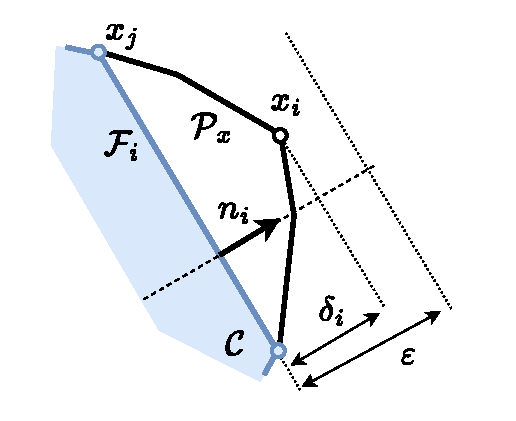
\includegraphics[width=\linewidth]{Papers/images/espilon_explicaiton.pdf}
    \caption{ The figure exemplifies the polytope face condition from equations (\ref{eq:normal_coplanar_test}) and (\ref{eq:normal_distance}), where  face $\mathcal{F}_i$ of the convex-hull $\mathcal{C}$ is considered to be the face of $\mathcal{P}_x$, because $\delta_i\! < \!\varepsilon$. }
    \label{fig:expilon_explication}
\end{wrapfigure}
\begin{equation}
    \bm{c}_i = \begin{cases}
  \bm{n}_i, & \text{if } \bm{n}_i^T(\bm{x}_{j} - \bm{x}_c) \geq 0, \\
  -\bm{n}_i, & \text{otherwise}.
\end{cases} 
\label{eq:normal_condition}
\end{equation}
Solving equation (\ref{eq:lin_prog}) with $\bm{c}_i$, the obtained $\bm{x}_i$ can be either a vertex of the polytope $\mathcal{P}_x$ or be coplanar with face $\mathcal{F}_i$. To determine if  $\bm{x}_i$ is coplanar with the face, a simple check can be devised, which verifies if the orthogonal (normal) distance from $\bm{x}_i$ to any vertex $\bm{x}_{j}$ of face $\mathcal{F}_i$
\begin{equation}
    \delta_i = \bm{n}_i^T(\bm{x}_{j} - \bm{x}_i)
\label{eq:normal_distance}
\end{equation}
is within a certain user defined accuracy $\varepsilon$:
\begin{equation}
    \bm{x}_i = \begin{cases}
   \text{vertex}, & \text{if }  |\delta_i| \geq \varepsilon, \\
    \text{on the face}, & \text{otherwise}.
\end{cases} 
\label{eq:normal_coplanar_test}
\end{equation}
Figure \ref{fig:expilon_explication} provides a graphical interpretation of this check and of the values $\delta_i$ and $\varepsilon$.

If $\bm{x}_i$ belongs to face $\mathcal{F}_i$ of the convex-hull $\mathcal{C}$ then  $\mathcal{F}_i$ is considered to be a face of the polytope $\mathcal{P}_x$. In that case the algorithm updates the $\repr{H}$-representation of $\mathcal{P}_x$ 
\begin{equation}
    H \leftarrow \begin{bmatrix} H \\ \bm{n}_i^T\end{bmatrix}, \quad \bm{d} \leftarrow \begin{bmatrix}  \bm{d} \\ \bm{n}^T_i \bm{x}_{j} \end{bmatrix}
\label{eq:h_rep}
\end{equation}
where $\bm{n}_i$ is the face normal vector and $\bm{n}_i^T \bm{x}_{j}$ is the orthogonal distance from the origin to the face $\mathcal{F}_i$. On the other hand, if $\bm{x}_i$ is a vertex of the polytope it is appended to the $\repr{V}$-representation list $\bm{x}_v \leftarrow [\bm{x}_v, ~\bm{x}_i]$.

\subsubsection{Stopping condition} 
\todos{Wrench/force ambiguity how do you represent them with the same unit}
Once all the faces of the convex hull $\mathcal{C}$ are evaluated, the convex hull is updated using the new vertex list $\bm{x}_v$.

One of the algorithm stopping conditions proposed by Bretl et al. \cite{Bretl2008}, is to construct the inner and outer approximation of the polytope $\mathcal{P}_x$ at the same time and stop approximating when the ratio $r=\vol{\mathcal{P}_{inner}}/\vol{\mathcal{P}_{outer}}$ between their volumes reaches certain threshold $r\leq1$.  

However, volume ratio condition is sometimes hard to interpret to the end-used, as its representation of the approximation error does not have the same units as the physical quantity being represented by the polytope $\mathcal{P}_x$. Therefore, the proposed algorithm exploits a different stopping condition setting the threshold on the maximal distance $\delta_i$. The algorithm stops iterating if the vertex list $\bm{x}_v$ has no new elements or, in other words, if the maximal distance $\delta_i$ for all the faces $\mathcal{F}_i$ is lower than the user defined accuracy $\varepsilon$  
\begin{equation}
    \max\{|\delta_{i}|\} \leq \varepsilon
\end{equation}
In this stopping condition, the maximal distance $\delta_i$ corresponds to the maximal error committed by the approximation, expressed with the same units as the units of the physical quantity being represented by the polytope. Preserving the same units improves the interpretation of the approximation error and enables the end-user to intuitively decide on the acceptable approximation error $\varepsilon$ for the application in question. 

Finally, if the user sets the approximation error $\varepsilon\!=\!0$ the proposed algorithm finds the exact solution, all the vertices and the faces of the polytope $\mathcal{P}_x$.

\subsection{Performance analysis}
\label{ch:chm_performance}

To evaluate the efficiency of the proposed approach, the challenging polytope formulation, corresponding to the generic formulation (\ref{eq:generic_polyt_view_revisit2}), with a high-dimensional input space and a low-dimensional output space ($n\gg m$) is tested. Additionally, the algorithm performance is compared against two state-of-the-art approaches: an approximation approach based on RSM algorithm introduced by Carmichael et al. \cite{carmichael_towards_2011} and an exact evaluation approach based on the combination of two efficient algorithms Hyper-plane shifting method \cite{hyper_psm} and Pivoting method \cite{bremner_fukuda_marzetta_1998}.

\subsubsection{Human wrench capacity polytope}
The polytope in question is the human's wrench capacity polytope, previously discussed in section \ref{ch:force_poly_human}. The polytope $\mathcal{P}_f$ characterising the achievable wrenches $\bm{f}$, the human can generate given its musculoskeletal model, can be expressed as 
\begin{equation}
    \mathcal{P}_f(\bm{q},\dot{\bm{q}},\ddot{\bm{q}}) = \left\{ \bm{f} \in \mathbb{R}^m ~|~ \bm{F}\in\left[\bm{F}_{min}, \bm{F}_{max} \right], ~~ \!J^T(\bm{q})\bm{f} =\! N(\bm{q})\bm{F} -\bm{\tau}_b(\bm{q},\dot{\bm{q}},\ddot{\bm{q}}) \right\}
    \label{eq:human_force_poly_revisit2}
\end{equation}
where $\bm{f}\in\mathbb{R}^m$ is the cartesian wrench, $\bm{F}\in\mathbb{R}^n$ is the vector of muscular forces, while $J(\bm{q})$ and $N(\bm{q})$ are configuration $\bm{q}$ dependant jacobian and moment arm matrix. Additionally, the bias vector $\bm{\tau}_b$ corresponds to the joint torques corresponding to the effects of the gravity and the movement. 

\begin{figure}[!t]
    \centering
    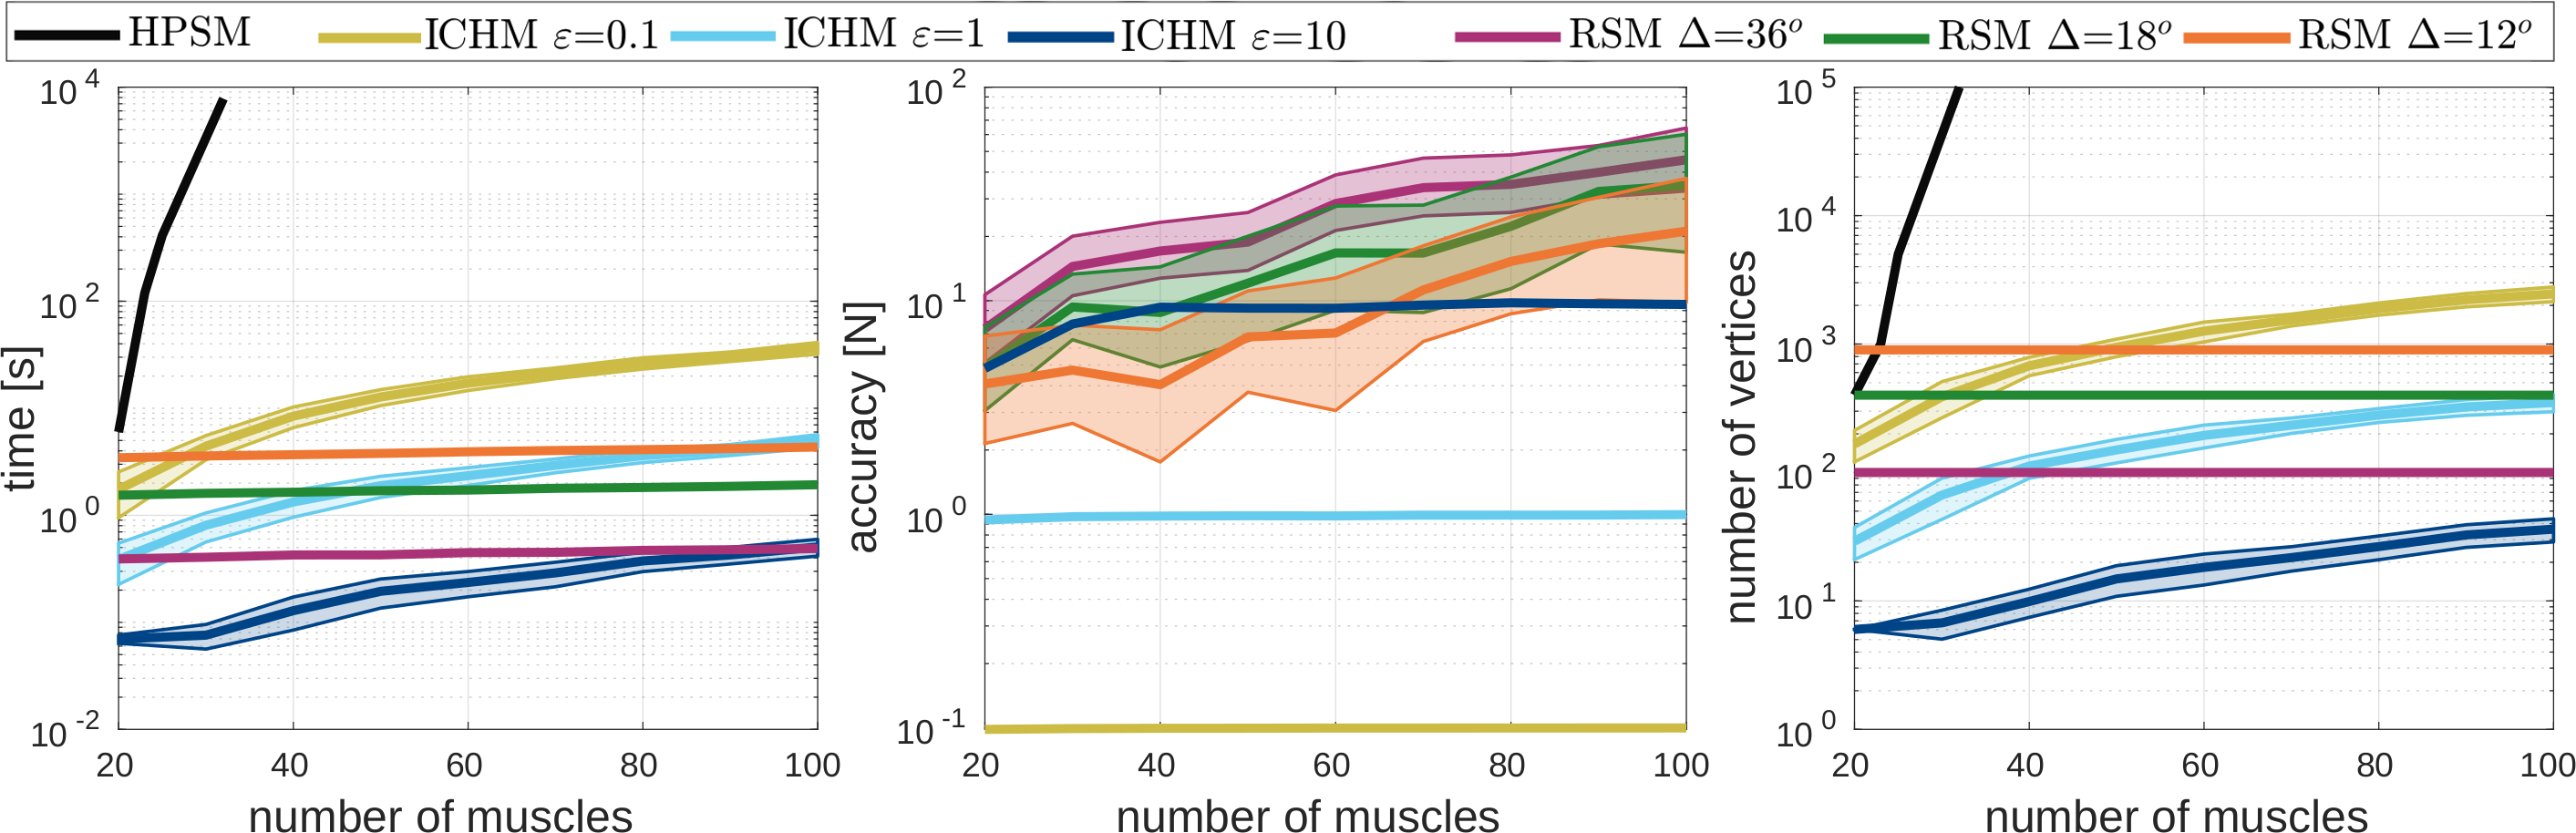
\includegraphics[width=1.\textwidth]{Papers/images/one_auto_new5_these}
    \caption{{Figure presenting the performance analysis results in the logarithmic scale for three different algorithms: HPSM, RSM and proposed CHM with respect to different number of muscles. Left figure shows the evolution of the execution time. Middle figure shows the evolution of the underestimation error, the maximal distance in between the polytope $\mathcal{P}_x$ and the acquired polytope, calculated as max$\{|\delta_{i}|\}$. Right figure shows the evolution of the number of vertices found. All the plots show the averaged results, with variances, over 100 runs, where each run corresponds to one randomly generated model.}}
    \label{fig:performance_results}
\end{figure}
This polytope formulation is challenging due to the high dimensional input space (large number of muscles), making the geometry of the polytope $\mathcal{P}_f$ relatively complex, having large number of faces and vertices. In such cases, standard exact methods for polytope transformation have long execution times, preventing this polytope representation to be used in interactive (online) applications. To reduce the computation times of the wrench polytope $\mathcal{P}_f$ evaluation, Carmichael et al. \cite{carmichael_towards_2011} have proposed an algorithm based on the Ray Shooting Method (RSM), described in section \ref{ch:approximation_algos}. Although the algorithm enables real-time approximation of the polytope $\mathcal{P}_f$, the obtained approximation is coarse and without any bounds on the approximation accuracy. 


\subsubsection{Experiment and results}
Therefore, to evaluate the performance of the proposed CHM algorithm, a comparative experiment is
performed, where the proposed algorithm's performance is compared against the RSM method proposed by Carmichael et al.\cite{carmichael_towards_2011} as well as against the two step exact approach based on the Hyper-Plane Shifting Method (HPSM)\cite{hyper_psm} and Pivoting method\cite{bremner_fukuda_marzetta_1998}. The experiment consists in finding the $\repr{V}$-representation of the cartesian force $m=3$ polytope $\mathcal{P}_f$ for a randomised mockup musculoskeletal model with $k\!=\!7$ degrees of freedom and a number of muscles ranging from $n$ = $20$ to $100$. 

The RSM algorithm \cite{carmichael2011Towards} requires uniform sampling of the ray directions in the 3D space. In this experiment the sampling is performed based on a two Euler angles parametrization. {For this method, three linearly increasing levels of granularity are tested for each Euler angle: $\Delta\!=\!36^o$, $18^o$ and $12^o$;  making for $n_r\!=\!10,20$ and $30$ rays per angle. Overall number of ray directions in 3D space ($N_r\!=\!n_r^2$) is then $100$, $400$ and $900$. For the proposed CHM algorithm, three exponentially increasing levels of accuracy are tested $\varepsilon\!=\!0.1$, $1$ and $10$ N.} All the algorithms are implemented in Matlab and run on a 1.90GHz Intel i7-8650U processor.

Results of the experiments, averaged over 100 algorithm runs, are shown on figure \ref{fig:performance_results}. The results confirm that the exact approach using the HPSM method has an execution time exponentially related to the number of muscles. Even for only 30 muscles it already takes more than 4.5 h to calculate, therefore this method is not tested on more than 30 muscles, where it finds over $10^4$ vertices.  

The RSM algorithm shows nearly constant time of execution for the full range of tested muscles and the constant number of vertices found, which is expected. The results show however, that for low muscle numbers $d\!<$25, when using a fine granularity $\Delta$=$12^o$ the RSM algorithm finds more vertices than the exact solution found by the HPSM. Furthermore, the middle plot of Figure \ref{fig:performance_results} shows that the RSM estimation error increases considerably with the number of muscles $d$, followed by a very
high variance. These results confirm that, as the polytope shape is not spherical, by uniformly covering the space of ray directions, RSM based algorithms will necessarily estimate certain areas of the polytope better than the others.

The graphs show that the proposed CHM method's execution time depends near-linearly of the number of muscles considered $d$ and the estimation error bound parameter $\varepsilon$. The accuracy graph, shown in the middle plot, shows that the proposed CHM algorithm is capable of limiting the estimation error of the polytope evaluation under desired value $\varepsilon$ regardless of the number of muscles. Furthermore, considering the vertex number found by the algorithms, it can be seen that the number of vertices has a nearly-linear relationship with the number of muscles $d$ and the variable $\varepsilon$. 

The demonstrated efficiency of the proposed CHM algorithm opens many doors for its applications in real-time systems, providing the user with an easy to understand trade-off between speed and accuracy.


\begin{figure}[!t]
    \centering
    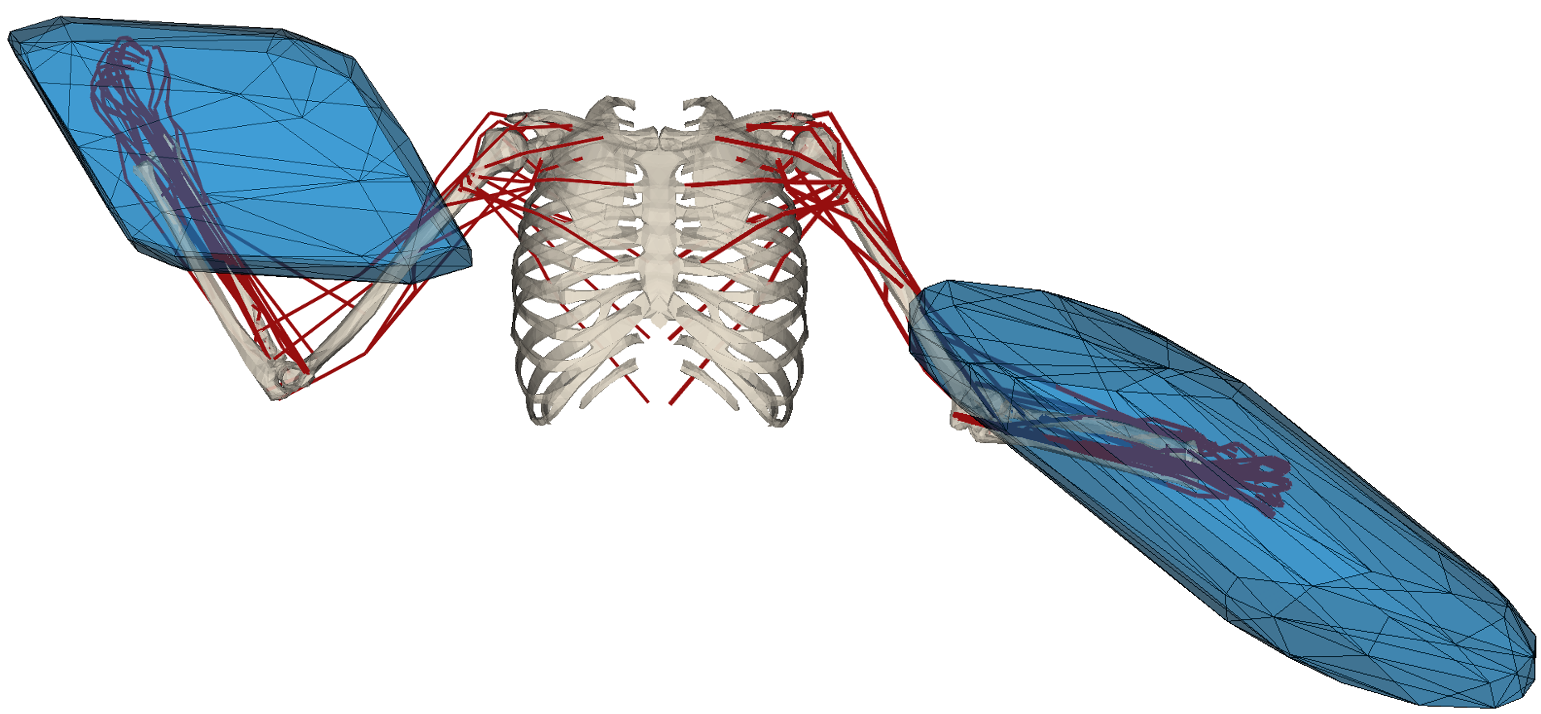
\includegraphics[width=0.5\linewidth]{Papers/images/bimanual.png}
    \caption{Cartesian force polytope of a musculoskeletal model of both human upper limbs  \cite{saul2015benchmarking} with 7Dof and 50 muscles each, visualised in \textit{pyomeca bioviz} \cite{Michaud2021}. The polytopes are scaled with a ratio 1m : 1000N}
    \label{fig:images_bimanual}
\end{figure}

\subsection{Algorithm summary}

In this section, a new algorithm for polytope approximation is introduced, developed for the generic polytope formulation
\begin{equation}
    \mathcal{P}_x = \big\{ \bm{x}\in \mathbb{R}^{m}\, |\,A\bm{x} = B\bm{y} + \bm{b}, \quad  \bm{y}\in\mathcal{P}_y  \big\}
    \label{eq:generic_polyt_view_revisit3}
\end{equation}
The algorithm is based on the Convex-Hull Methods (CHM) \cite{lassez1992quantifier}, described in section \ref{ch:approximation_algos}. The proposed CHM algorithm approximates the polytope $\mathcal{P}_x$, refining the approximation iteratively until the approximation error is reduced within user defined level. 
Additionally, the proposed algorithm finds the $\repr{V}$ and $\repr{H}$-representation of the polytope $\mathcal{P}_x$ at the same time and therefore.

The proposed algorithm is \textit{output sensitive}, where its complexity depends directly on the number of vertices and faces of the polytope  $\mathcal{P}_x$. By allowing the user to define the desired level of the approximation accuracy $\varepsilon$, the user can effectively simplify the polytope $\mathcal{P}_x$ geometry, lower the number of faces and vertices, and reduce the overall execution time. 
The approximation accuracy $\varepsilon$ represents the maximal distance from the obtained polytope approximation and furthers vertices of the polytope $\mathcal{P}_x$ and has the same unit as the physical quantity represented by the polytope. 
Therefore, by choosing the appropriate value $\varepsilon$ for a given application the user can intuitively trade-off the approximation accuracy for the execution time, and in many cases bring it to the interactive (online) range. 

\begin{algorithm}[!b]
\caption{Proposed CHM algorithm pseudo-code}
\begin{algorithmic}
\REQUIRE $A$,$B$, $\bm{y}_{min}$, $\bm{y}_{max}$, $\bm{b}$, $\varepsilon$
\STATE $U, \Sigma, V^T \leftarrow svd(A^+)$ 

\STATE init $\repr{H}$-rep: $H,\bm{d} \leftarrow [\,]$ and $\repr{V}$-rep: $\bm{x}_v,\bm{y}_v\leftarrow [\,]$
\STATE \textbf{for all}   {$\bm{u}_i$ in $U$} \textbf{do}

\hspace{0.3cm} $\bm{y}_{i}\leftarrow$ LP (Eq. \ref{eq:lin_prog}) with $\bm{c}\! =\! \bm{u}_i$ and $\bm{c}\! =\! -\bm{u}_i$

\hspace{0.3cm} $\bm{x}_{v} \leftarrow [\bm{x}_{v}, ~ A^+B\bm{y}_i + A^+\bm{b}]$

\REPEAT

\STATE calculate the convex hull $\mathcal{C}$ of $\bm{x}_{v}$
\STATE calculate the centroid $\bm{x}_{c} = \frac{1}{N}\sum_i\bm{x}_{v,i}$

\STATE \textbf{for all}   {new face $\mathcal{F}_i$ in $\mathcal{C}$} \textbf{do}
%\FORALL{ new face $\mathcal{F}_i$ in $\mathcal{C}$ } 

\hspace{0.25cm} find normal $\bm{n}_i$ and one vertex $\bm{x}_{j}$ of $\mathcal{F}_i$

\hspace{0.25cm} $\bm{y}_{i}\leftarrow$ LP ( Eq. \ref{eq:lin_prog} ) with  $\bm{c}\! =\! \bm{n}_i$ ( Eq. \ref{eq:normal_condition} )

\hspace{0.25cm} $\bm{x}_{i} = A^+B\bm{y}_i+A^+\bm{b}$ 

\hspace{0.25cm}  calculate $\delta_i$ (Eq.\ref{eq:normal_distance})

\hspace{0.25cm}  \textbf{if}   $ |\delta_i| \leq \varepsilon$ \textbf{then} 

\hspace{0.6cm}  new face: update $\repr{H}$-rep  ( Eq. \ref{eq:h_rep} )

\hspace{0.25cm}  \textbf{else}

\hspace{0.6cm} new vertex: update $\repr{V}$-rep: $\bm{x}_{v} \!\leftarrow\! [\bm{x}_{v},~ \bm{x}_i ]$,  $\bm{y}_{v} \!\leftarrow\! [\bm{y}_{v},~ \bm{y}_i ]$ 

%\ENDFOR
\UNTIL{{ $\max\{|\delta_{i}|\}\leq \varepsilon$}}
\RETURN  $\repr{V}$-rep: $\bm{x}_v$, $\bm{y}_v$ and  $\repr{H}$-rep: $H$, $\bm{d}$ 
\end{algorithmic}
\label{alg:algo_2}
\end{algorithm}

As discussed in section \ref{ch:collab_metrics_overview}, the generic polytope formulation (\ref{eq:generic_polyt_view_revisit3}) unifies the formulations of all the common polytope characterisations of human's and robot's physical abilities, making the algorithm applicable to the transformation of all of their polytope formulations described in section \ref{ch:poly_metrics}. Even thought the algorithm can be applied to all the polytope formulations corresponding to (\ref{eq:generic_polyt_view_revisit3}) and its special cases, it is particularly well suited for cases where the dimension of the input space is high ($n\gg m$) and the dimension of the output space is relatively low ($m\leq3$), as it directly searches for the vertices and faces of the polytope $\mathcal{P}_x$ in the low dimensional output space. 

Such high-dimensional ($n\gg m$) polytope enumeration problems are challenging for the standard polytope transformation methods, described in section \ref{ch:polytope_algorithms}, however relatively common when it comes to polytope representation of physical abilities of human's based on their musculoskeletal models. The polytopes based on human musculoskeletal models have therefore been limited to the off-line execution \cite{biomechanics1010008} and in many cases subject to coarse simplifications \cite{carmichael_estimating_2013}. As shown in the experimental results, in section \ref{ch:chm_performance}, the proposed algorithm substantially improves the time execution of finding the $\repr{V}$ and $\repr{H}$-representation of the challenging formulation of the human wrench capacity polytope while at the same time guaranteeing the user defined level of accuracy $\varepsilon$. The results show, that the proposed algorithm is capable of calculating the vertices of this polytope within a half of second for the human musculoskeletal models up to 100 muscles (while guaranteeing the precision of 10$N$) which opens many doors for real-time applications, for example for human-centred robot control in robotics. 

The pseudo-code of the proposed algorithm is given in Algorithm \ref{alg:algo_2}, while an efficient open-source python implementation is publicly available within the package \textsc{pycapacity}\footnote{https://auctus-team.github.io/pycapacity/}, which is described more in detail in chapter \ref{ch:software}.

Finally, section \ref{ch:human_robot_carrying} brings the application of the proposed algorithm for the real-time robot control in the human-robot collaboration scenario, where the algorithm is exploited in order to calculate the human's wrench capacity polytope online. 

\section{Conclusion}

This chapter aimes to provide a set of tools for efficient transforming of polytopes representing the physical abilities of humans and robots into more standardised forms suitable for practical applications. The focus is put on the two widely used polytope representations: vertex or $\repr{V}$ and half-plane or $\repr{H}$-representations. These representations offer various advantages, including compatibility with visualisation tools, in a for triangulated meshes, and optimisation-based applications like robot control and trajectory planning. Additionally, they enable efficient operations like Minkowski sums and intersections over multiple polytopes.

While the literature presents numerous algorithms for transforming polytope formulations into their $\repr{H}$ or $\repr{V}$-representation, these algorithms are often tailored to specific sets of polytope formulations. The previous chapter proposed a generic view on different common polytope representation of humans' and robots' physical abilities and proposed a unifying polytope formulation describing all the proposed metrics, introduced in section \ref{ch: collab_metrics_overview}. However, this unified formulation is not directly suitable for the standard polytope transformation algorithms. Hence, section \ref{ch:generic_view} proposes a structured view on different polytope formulation families derived from the proposed generic unified formulation namely intersection and projection formulation, as well as some special cases.

Section \ref{ch:polytope_algorithms} further provides an overview of applicable techniques for transforming these families into their $\repr{V}$ or $\repr{H}$-representation. The chapter briefly introduces the standard generic methods for mutual transformation between $\repr{V}$ and $\repr{H}$-representation, followed by the polytope formulation specific methods that are capable of better exploiting the geometry of the formulation families. Finally, several polytope approximation methods are discussed as a means of improving the efficiency of polytope transformation for high-dimensional problems. 
The aim of this overview is to provide a brief introduction into the applicable state-of-the-art methods when it comes to transforming different polytope formulations as well as to discuss their limitations and computational efficiency.

The final two sections of this chapter bring introduce two contributions of this thesis in the domain of polytope transformations. The section \ref{sec:algorithm_vea} introduces an efficient vertex enumeration algorithm for the intersection polytope formulation with the interval input set. This algorithm is based on the work by Sasaki et al~\cite{sasaki2011vertex}, exploiting the geometry of the hyperrectangle input set in order to improve its computational complexity of its exhaustive search and reduce the execution time. The algorithm is particularly well suited for low dimensional polytope evaluation, that are common when it comes to polytope characterisations of physical abilities of robotic manipulators. The performance of the proposed algorithm is compared to the state-of-the-art methods on finding the $\repr{V}$-representation of the force capacity polytope for redundant robotic manipulators, introduced in section \ref{ch:poly_force}. The results show that the algorithm has significantly lower computational complexity and hence shorter execution time, in the order of magnitude of several milliseconds for standard robotic manipulators, implemented in Pyhton. Such short execution time opens doors for using these polytopes in real time applications, such as robot control. 

Section \ref{ch:algorihtm_ichm} brings a new polytope approximation algorithm based on the Convex-Hull Method (CHM) by lassez et al. \cite{lassez1992quantifier}. The algorithm is developed for the generic polytope formulation directly and can therefore be used with all the common polytope formulation introduced in previous chapter. This algorithm performs an iterative approximation of the final polytope by using sequences of Linear Programming (LP) to find new vertices of the polytope and Convex-Hull to group the to faces. The algorithm improves the approximation accuracy in each iteration and continues iterating when desired user defined approximation accuracy is reached. The execution time of the algorithm depends directly of the complexity of the polytope being transformed (number of faces and verteices), therefore by appropriately setting the desired accuracy, the algorithm is capable of simplifying the final geometry of the polytope and lowering the execution time. This is particularly useful when it comes to the high-dimensional problems, where the input space dimension is much higher than the output space $n\!\gg \!m$, where the standard exact methods have intractable execution times, as they are based on different forms of the exhaustive search. Such high-dimensional problems are very common when it comes to characterising physical abilities of humans based on their musculoskeletal models, as they often have large number of muscles $n$, while their capacities are characterised in the cartesian space $m=3$. The performance of the proposed method is therefore tested on the challenging polytope formulation of the human's wrench capacity polytope, described in section \ref{ch:force_poly_human}. The results of the proposed methods in comparison to the state-of-the-art methods show that it has significantly shorter computation time while at the same time guaranteeing the user defined approximation accuracy. Furthermore, the results show that the porpoised algorithm, in the case of human's wrench capacity polytope, has execution time under half of a seconds for musculoskeletal models up to 100 muscles, opening many doors for using this polytope formulation in the real time applications.

Following chapter leverages the proposed algorithms and formulations to propose several use-cases of the polytope based physical ability characterisations in the context of the real-time robot control in different human robot physical collaboration scenarios. Chapter \ref{ch:topca} proposes a new cartesian space trajectory planning strategy exploiting the polytope algebra, while chapter \ref{ch:hfr} introduces a new polytope based approximation of the robot's reachable space within a horizon. Finally, chapter \ref{ch:software} presents the publicly available open-source software package implementing several algorithms introduced in this section and enabling an efficient, real-time compatible, evaluation of polytope based physical abilities for humans and robots.
